\documentclass[12pt]{article}
\usepackage[utf8]{inputenc}
\usepackage{amsmath,amssymb,hyperref,array,xcolor,multicol,verbatim,mathpazo}
\usepackage[normalem]{ulem}
\usepackage[pdftex]{graphicx}
\usepackage{fullpage}
\usepackage{import}
\usepackage{adjustbox}
\usepackage{booktabs}
\usepackage{bbm}
\usepackage[font=normalsize,labelfont=bf]{caption}
%\captionsetup{justification=raggedright,singlelinecheck=false}
\usepackage{subcaption}
\usepackage{pdflscape}
\usepackage{threeparttable}
\usepackage{makecell}

\usepackage[backend=biber,style=authoryear,citestyle=authoryear, natbib=true]{biblatex}
\addbibresource{papercitations.bib}
\usepackage{setspace}
\onehalfspacing
\addtolength{\skip\footins}{2pc plus 5pt}

\usepackage{geometry}
 \geometry{,
 left=25.4mm,
 top=25.4mm,
 right=25.4mm,
 bottom=25.4mm
 }

 \renewcommand{\TPTnoteSettings}{\footnotesize}
 


\DeclareLabeldate[online]{%
  \field{date}
  \field{year}
  \field{eventdate}
  \field{origdate}
  \field{urldate}
}
\usepackage{times}


\begin{document}

\linespread{1.2}\title{\vspace{-0.5in} Labor Markets and Technological Change: \\ \Large Evidence from Electronic Health Records%\thanks{I thank Ian McCarthy for his continued advice and guidance, along with the additional faculty and graduate students at Emory University for their feedback. Additionally, I would like to thank discussants and conference attendees at the Young Economist Symposium and American Society of Health Economics for their helpful suggestions.}
}  
	
	%\date{\today}
	
	%\author{\vspace{10mm}Hanna Glenn\footnote{School of Economics, University of Queensland, hanna.glenn@uq.edu.au.}}
    
	
	\maketitle
	%\setlength{\droptitle}{-10pt}
	
	\vspace{-0.2in}
	
	\singlespacing\maketitle

\begin{abstract}\small
    Technology adoption in healthcare has the potential to improve patient outcomes, and in some cases, decrease costs. However, new technology can also impose new burdens on providers. In this paper, I investigate changes in physician labor market behavior following the adoption of electronic health records (EHRs), a major technological shift in healthcare spanning 2009--2015. Treating hospital EHR adoption as an exogenous shock to hospitalists, I use staggered difference-in-differences to estimate the effect of EHRs on hospitalists' decisions to remain in clinical practice, their work setting, and their productivity. I show that hospitalists of retirement age are more likely to leave clinical work after EHR exposure, and those who remain in clinical practice shift work towards office settings. For hospitalists that do not shift towards office work, EHRs lead to a modest increase in patients seen. These findings inform the full costs and benefits of technology adoption in healthcare, which are especially important in a rapidly evolving technological environment.
\end{abstract}

\vspace{2.5in}
	
	\noindent Keywords: Electronic Health Record, Physician Behavior, Technology Adoption

    \vspace{2mm}
	
	\noindent JEL Codes: I11, J24, O33

	
	\onehalfspacing
	
	\newpage

\section{Introduction}

Technological innovation has long reshaped work by changing labor demand, wages, and how production is organized. In healthcare, new technologies also affect patient outcomes, making it especially important to understand how policy shapes their implementation. One of the most widespread technology roll-outs across healthcare facilities in the U.S. was the electronic health record (EHR), computer systems that house digital medical records with the capability to be used for more complex functionalities. EHRs became increasingly relevant after 2009, when the HITECH Act subsidized hospitals and practices to ``meaningfully'' use EHRs (\cite{hitech}).\footnote{Meaningful use (MU) standards proceeded in three stages. Stage 1, which began in 2011, focused on electronic data capture and sharing. Stage 2, finalized in 2012 and effective from 2014, extended MU to health information exchange, clinical processes, and patient engagement. Stage 3, introduced in 2017 and required from 2018, focused on using EHRs to improve health outcomes (\cite{meanuse}).} President Obama stated in 2009, “To improve the quality of our healthcare while lowering its cost, we will make the immediate investments necessary to ensure that, within five years, all of America’s medical records are computerized.” (\cite{presquote}). The strong incentives for EHR use stemmed from a widespread expectation that EHRs would improve quality of care while decreasing costs, the gold standard in health policy. For example, a 2005 study estimated hundreds of billions of dollars saved if health information technology were to be fully implemented (\cite{hillestad2005}).

Prior to 2009, many EHRs were used only for data management and storage. However, the government-incentivized functionalities were heavily physician-facing, making physicians the primary factor in whether the expected benefits were realized. Because a new system can alter daily workflows, some physicians “loathe the cumbersome, time-consuming data entry that comes with using EHR.” (\cite{CollierBurnout}). Among hospitalists, 63\% of survey respondents found EHRs time consuming and inefficient (\cite{czernik2022hospitalist}). Learning a new, potentially burdensome system raises the cost of working in settings that use it, while any productivity gains accrue only to physicians who continue to use it. Physicians with less to gain, such as those nearing retirement, may respond by exiting the labor market altogether or shifting towards alternative work settings. The extent to which these costs are meaningful is unknown, making physician response an empirical question. A hospital's decision to adopt an EHR is plausibly exogenous to hospitalists. Thus, I use a difference-in-differences research design to estimate the effect of hospital EHR adoption on hospitalist labor market choices: (1) exiting clinical work altogether, measured based on no future claims, (2) substituting inpatient work to offices, measured by the location of claims, and (3) care/billing patterns, measured by the number of patients seen and claims filed per patient.

While hospitalists are an ideal setting to answer this question econometrically, they are also important in their own right. Approximately 44,000 physicians are employed as hospitalists in the U.S. (\cite{bls}), and one third of Medicare admissions are seen by a hospitalist (\cite{messler2015history}). I combine several data sources to construct a panel of hospitalists spanning from 2009--2017. Using Centers for Medicare and Medicaid Services (CMS) Shared Patient Data, I identify the hospital affiliation of each hospitalist. I use both the American Hospital Association (AHA) Survey and Health Information and Management Systems Society (HIMSS) to determine hospital adoption of physician-facing EHR functionality, and thus connect hospitalists to EHR exposure. Finally, I use Medicare Data on Provider Practice and Specialty (MD-PPAS) for physician-level practice information. The independent variable of interest is binary, capturing exposure to an EHR. I estimate average group-time treatment effects of EHR exposure on physician labor market behavior (\cite{callaway2021difference}).

EHR exposure increases the probability that a hospitalist exits clinical work by 1.3 percentage points, driven by physicians near retirement age. Removing those who exit, EHR exposure leads remaining hospitalists to increase the share of claims delivered in an office setting by 11 percentage points, a shift that is largest among hospitalists contracted through staffing companies and is accompanied by movement away from staffing arrangements and toward independent practice. The office-based results are robust to a range of sensitivity checks, including accounting for selection into each relevant sample, bounding the sensitivity of the estimates to violations of parallel trends, and testing alternative estimators and sample thresholds; the exit results are directionally consistent across these checks but less precise. Finally, for hospitalists who do not change work setting, EHR exposure increases the number of patients seen by about 18 per year on average over the four years following exposure, roughly 5\% of the pre-exposure mean, consistent with productivity gains accruing to those who continue using the technology. This increase is large enough to suggest that it reflects more than a simple redistribution of patients from physicians who left clinical settings, although the estimate is more sensitive to specification choices.

This paper contributes to our understanding of the effects of health information technology. Despite a large number of case studies that find improved patient outcomes and decreased cost (surveyed in \cite{Buntin2011TheResults}), quantitative studies have found more mixed results: outcomes for median patients do not change as a result of EHRs (\cite{Agha2014TheCare}, \cite{McCullough2016HealthCoordination}, \cite{Meyerhoefer}) newborns and severe patients experience improvement in health outcomes (\cite{Miller2009}, \cite{Freedman2015}, \cite{McCullough2016HealthCoordination}), and hospital costs only decrease six years after implementation, if at all (\cite{Agha2014TheCare}, \cite{dranove2014trillion}). Relating EHRs to productivity, one study finds that nursing home productivity increases after adopting health IT (\cite{Hitt2016}), but another finds that physician productivity decreases by 11 percent due to EHRs being adopted in primary-care sites (\cite{Meyerhoefer}). Most related to this paper, \citet{lin2026health} finds that health IT diffusion increased hospital-based physician density, with growth concentrated among early-career physicians, and a related study of Florida physicians shows that EHR implementation influences physician mobility, with more disruptive implementations increasing physician departures (\cite{greenwood2019does}). I contribute to this literature first by considering the full range of individual physician labor market decisions as outcomes, which, to my knowledge, has not yet been examined in this setting. Further, I consider the primary time period in which physician-facing EHRs were rapidly implemented, in part due to the HITECH Act (\cite{dranove2015investment}). Similar to past studies, I utilize EHR adoption as the treatment variable in a difference-in-differences framework, and I improve on past strategies by estimating group-time treatment effects, avoiding problems in typical two-way fixed effects models with staggered treatment.

The paper is organized as follows. Section \ref{sec:background} provides background on EHR adoption in the U.S. and hospitalist incentives. Section \ref{sec:data} outlines the data and provides summary statistics. Section \ref{sec:empstrat} details the empirical strategy and identification assumptions. Section \ref{sec:results} contains the results and discussion of threats to validity. 




\section{Background}\label{sec:background}

\subsection{EHRs and Meaningful Use}
EHRs have been an important feature of healthcare since the 1980s. Early in their existence, healthcare professionals perceived the technology as a complement to paper records, primarily deployed by large academic medical centers to improve billing and scheduling efficiency. Physicians did not interact directly with these early-generation EHRs and thus were not drastically affected by their implementation. As innovation made computers more portable, EHR usability increased, creating what is known as the ``physician workspace'': a computer station for physicians to interface directly with an EHR to record patient updates. Despite usability improvements, physicians continued to view EHRs as complementary to paper due to burdensome data entry (\cite{evans2016electronic}).

The HITECH Act, passed in 2009, designated \$27 billion in subsidies to entities using EHRs according to specific guidelines. Subsidies were tied to three stages of requirements: Stage 1 (2011) focused on data capture; Stage 2 (2014) extended to health information exchange and clinical processes; and Stage 3 (2017) focused on improving health outcomes. Hospitals without EHRs by 2015 faced penalties of lower Medicare reimbursements. Widespread EHR adoption coincided with the roll-out of these subsidies: the share of non-federal acute care hospitals with at least a basic EHR rose from under 10 percent in 2008 to 84 percent in 2015 \citep{henry2016adoption}. However, subsidies did not necessarily cause all adoption. \citeauthor{dranove2015investment} (\citeyear{dranove2015investment}) estimate adoption would have been ten percentage points lower without the policy. Figure~\ref{fig:meanuse} shows a geographical comparison of hospitals receiving Stage 1 subsidies in 2011 vs. 2013, illustrating the nationwide expansion of the technology.

Primary care physicians spend 5.9 hours of an 11.4-hour workday in the EHR, nearly two hours for every hour of direct patient care. Clerical and administrative tasks, including documentation and order entry, account for 44\% of that time, and inbox management for another 24\% \citep{arndt2017tethered}. Despite the time spent, physicians continue to report frustration over EHR use. The most time-consuming functions are also reported as the most frustrating (\cite{dymek2021building}). Hospitals often provide training upon adoption, but rapid upgrades and changes make familiarity difficult. While these studies focus on outpatient settings, the limited research on hospitalists shows similar patterns (\cite{tipping2010did}). Together, these findings suggest that EHR adoption imposes a meaningful, ongoing cost to physicians, one that could plausibly affect decisions about whether, and where, to continue practicing.

\subsection{Hospitalists and Labor Market Decisions}

This section outlines the potential responses of hospitalists to EHRs based on their incentives and institutions. The behaviors considered are closely related and should not be taken as independent. For example, hospitalists' choice of work setting depends on their decision to remain in clinical practice, and billing activity depends on work setting. Thus, I discuss the behaviors as a progression of decision making. For the purposes of this paper, I define a hospitalist as any general practice physician who sees at least 70\% of their patients in a hospital setting. 

\subsubsection{Exiting Clinical Work}

Physicians can stop seeing patients either by retiring or switching to non-clinical careers. While retirement decisions are typically planned and financially driven (\cite{gustman1986disaggregated}; \cite{stock1990pension}), physicians often delay retirement for altruistic reasons such as maintaining patient relationships (\cite{collier2017challenges}). Thus, the option to retire may exist for years before a physician actually exits clinical practice. Age plays a central role, where older physicians have less time to benefit from learning a new system, making them more likely to be influenced by technology shocks like EHR adoption. If EHRs reduce job satisfaction, they may induce physicians, especially those near retirement, to leave clinical work. Alternatively, if EHRs improve daily tasks, they may encourage continued practice. Media accounts suggest that EHR implementation prompted physicians to retire (\cite{ringel_2019}; \cite{loria_2020}), though this remains empirically untested.

Physicians of any age may also leave clinical roles for careers in administration, teaching, consulting, or hospital management. While early career physicians are unlikely to fully retire, they may still leave clinical work if EHRs reduce job satisfaction. In a 2016 survey, 13\% of physicians reported considering non-clinical careers due to burnout (\cite{physicians2016physicians}). I observe only whether a physician stops seeing Medicare patients, not whether they retire or career switch. Thus, for the purposes of this paper, exit indicates no longer seeing patients, encompassing both formal retirement and career switching.

\subsubsection{Work Setting}\label{sec:worksetting}

For physicians who remain in practice, EHR adoption may affect the setting in which they choose to work. Specifically, if EHRs affect job satisfaction in hospitals, a hospitalist may shift working hours toward or away from inpatient care. This margin is potentially important because many hospitalists divide their time across multiple settings. A 2013 survey estimated that 36\% of hospitalists also worked outside the hospital in primary care, long-term care, or hospice settings (\cite{Today}). Although office and inpatient services are not fully interchangeable, changes in claims from hospital to office settings can signal shifts in where physicians choose to practice.

The interpretation of such shifts depends in part on physicians' employment arrangements. Hospitalists are heterogeneous in their relationships with hospitals. Some are employed directly by the hospital, while others work through staffing companies that contract with hospitals to provide inpatient coverage. These arrangements differ in who controls physician assignments and how adjustments to staffing are made. As a result, a change in work setting may reflect a physician's own response to EHR adoption, a hospital's staffing decisions, or some combination of the two.

Hospitalists employed directly by a hospital may be reassigned within the hospital system, including to affiliated outpatient facilities. For these physicians, a shift in work setting may therefore reflect internal staffing decisions as opposed to physician preferences. By contrast, physicians working through staffing companies often provide inpatient services through a contractual arrangement with a particular facility. Changes in work setting for these physicians are less likely to arise from internal hospital reallocation and more likely to reflect changes in contractual arrangements or physician choices regarding where to provide care. Because they may provide coverage across facilities, these physicians may also expect less benefit from learning any one hospital's system. Physicians in solo or independent practice generally have greater discretion over where they work, although independence exists on a spectrum because physicians may simultaneously maintain an independent practice and provide inpatient services through staffing arrangements.

My sample includes both salaried hospitalists and physicians who split time across settings. Although I cannot observe individual physician contracts with each hospital, I use proxy information on the physician's primary organization through which they receive payment to explore whether shifts in work setting reflect physician or employer-driven decisions.

\subsubsection{Care/Billing Activity}

For hospitalists who remain in inpatient practice throughout the sample period, it is natural to assess whether EHR exposure affected patient care patterns. A central goal of the HITECH Act was to improve the efficiency of care by reducing administrative burdens, which could manifest as physicians seeing more patients or documenting care more efficiently. At the same time, EHRs could add new daily tasks that hinder rather than enhance productivity. I cannot directly assess productivity in the sense of quality-adjusted output, since I lack granular information on how care is shared among providers treating the same patient or how physicians allocate their time across tasks; a physician seeing more patients could reflect greater efficiency, but could also reflect less time spent per patient or a change in how care is divided among providers. I instead observe total patient volume, which captures one aspect of productivity even though it cannot distinguish between these explanations. Whether any resulting change in patient volume affects patient welfare is outside the scope of this paper.

EHRs may also influence hospitalist billing behavior, and plausibly in offsetting directions. Physicians often over-treat patients due to defensive medicine concerns, patient demand, or limited access to a patient's full medical history (\cite{lyu2017overtreatment}). By improving access to a patient's existing records and test results, EHRs could reduce this kind of over-treatment, lowering the number of repeated or unnecessary tests and, in turn, the number of claims filed per patient. On the other hand, more detailed digital documentation may also make it easier for hospitals and physicians to justify higher-complexity billing codes for the same underlying care, a practice sometimes referred to as EHR-enabled upcoding. Under this channel, EHR adoption could increase claims per patient even absent any change in the underlying volume or intensity of care provided.



\section{Data}\label{sec:data}

I construct a balanced hospitalist-level panel data set spanning from 2009--2017 which measures physician exposure to EHRs over time, several labor market outcomes, and other physician and hospital characteristics. I describe the different data sources used to construct the panel below, and I include a detailed outline of data and variable construction in Appendix \ref{app:data}.

\subsection{Sample Construction}\label{sec:sample}

I first gather physician information from Medicare Data on Provider Practice and Specialty (MD-PPAS), a provider-level database CMS constructs from provider enrollment records and the 100 percent file of Original Medicare Part B non-institutional claims. It reports provider demographics, specialty, patient demographics, and the share of claim line items delivered in several places of service. Patient counts therefore capture traditional fee-for-service Medicare. I only include physicians classified as hospitalists, internal medicine, general practice or family practice. I drop physicians with consistently less than 70\% of patients in a hospital setting, as the focus is on physicians with sufficient exposure to hospitals.\footnote{I consider thresholds of 50\% and 90\% as robustness checks in Appendix \ref{sec:changes}.}

For precise information on which hospitals each physician is working in, I utilize the 2009-2015 CMS Shared Patient Data files, which provide information on how often the same patient is seen by different providers. For example, when a primary care physician refers a patient to a specialist, the two providers become a pair who share at least one patient. I focus on shared patients within the same day between physician and hospital entities. To refine the sample, I restrict to physician-hospital pairs with non-missing tax codes and at least 30 same-day shared patients per year.\footnote{I consider thresholds of 10 and 60 as robustness checks in Appendix \ref{sec:changes}.} This allows me to exclude office-based primary care physicians and ensures consistency with physicians identified in the MD-PPAS dataset. 

MD-PPAS also reports the legal name of the taxable organization (TIN) under which each physician predominantly bills. Because Medicare requires claims to be billed under the TIN of the employing or contracting organization rather than the individual physician, this variable identifies the organization name receiving payment on each hospitalist's behalf, which need not be the hospital where they physically practice. I use string detection to classify each hospitalist's primary employer entity type into one of three categories: (1) hospital-affiliated, where the physician bills under the name of the hospital itself or an affiliated health system; (2) staffing company, where the physician is contracted through a third party rather than employed by the hospital or system directly; and (3) independent, where the billing name is the physician's own name or has a small-practice legal suffix (e.g., LLC, PC, PA). 

I link hospitals within each pair to two sources of EHR adoption information: the American Hospital Association (AHA) survey and the Healthcare Information and Management Systems Society (HIMSS) survey. In the AHA Annual Survey, hospitals are asked to classify their Electronic Health Record status and respond with 0: not implemented, 1: partially implemented, or 2: fully implemented. In the HIMSS survey, hospitals are asked granular questions about their health information technology use, including which applications within the EHR are ``Live and Operational". In the 2009-2015 time period, the possible applications are clinical data repository, clinical decision support, computerized practitioner order entry (CPOE), physician documentation, and physician portal. 

In Table \ref{tab:ehr_construct}, I present all possible combinations of hospital responses across the AHA and HIMSS data sources. Comparing the two sources shows that full EHR implementation in the AHA data aligns more closely with physician-facing applications than with back-end applications in HIMSS. This pattern suggests that hospitals do not view back-end applications alone as constituting a fully implemented EHR. Accordingly, I classify a hospital as having adopted an EHR whenever either source indicates adoption: if the AHA reports full implementation or if HIMSS records a physician-facing application (computerized physician order entry, physician documentation, or a physician portal). Additional details on the construction of the EHR adoption measure are provided in Appendix \ref{sec:hosplevel}.

I limit to hospitalists who graduated before 2005, as anyone who graduated medical school after that will be finishing residency during the span of the data and will exhibit labor market changing behavior. I also exclude hospitalists affiliated with hospitals that are acquired at the same time as EHR exposure. Because the shared-patient data used to construct physician-hospital pairs end in 2015, I observe treatment only through 2015 and drop anyone not treated by then. The estimation sample therefore contains no never-treated units, and identification comes from comparisons with hospitalists not yet exposed. As a result, group-time effects are identified only through 2014, the last year with not-yet-exposed hospitalists. I nonetheless retain outcome data for 2016 and 2017 because the exit outcome requires observing whether a hospitalist bills in any later year. This also yields a better comparison group: given the strength of the Meaningful Use incentives over this period, hospitals that had still not adopted an EHR by 2015 are likely to differ substantially from those that did. Appendix~\ref{sec:nevertreated} shows that the two groups differ significantly in age, hospital size, and baseline practice setting, and that estimates using never-treated comparisons are difficult to interpret as treatment effects.

Because the outcomes I study form a progression of decisions, I estimate each set of outcomes on a separate sample. The exit sample includes all 5,471 hospitalists described above and is not restricted on any outcome. For the work-setting outcomes, the sample excludes hospitalists who exit clinical practice during the sample period, since work setting is not observed after exit, leaving 4,798 hospitalists. For patient volume and claims per patient, the sample further excludes hospitalists who shift more than 30\% of their patients to an office setting, so that the remaining hospitalists continue to practice in, and use the EHR of, the hospital throughout the sample period. This leaves 2,237 hospitalists. Because the office and productivity samples condition on outcomes that EHR exposure may itself affect, estimates from these samples could be biased by selection, and I report Lee (2009) bounds for these outcomes in Appendix \ref{sec:leebounds}. Figure \ref{fig:cohortsizes} shows the number of hospitalists first exposed to an EHR in each year for each sample.

\begin{figure}[ht!]
\centering
\captionsetup{width=.9\linewidth}
    \caption{Number of Hospitalists by Year of First EHR Exposure and Estimation Sample}
    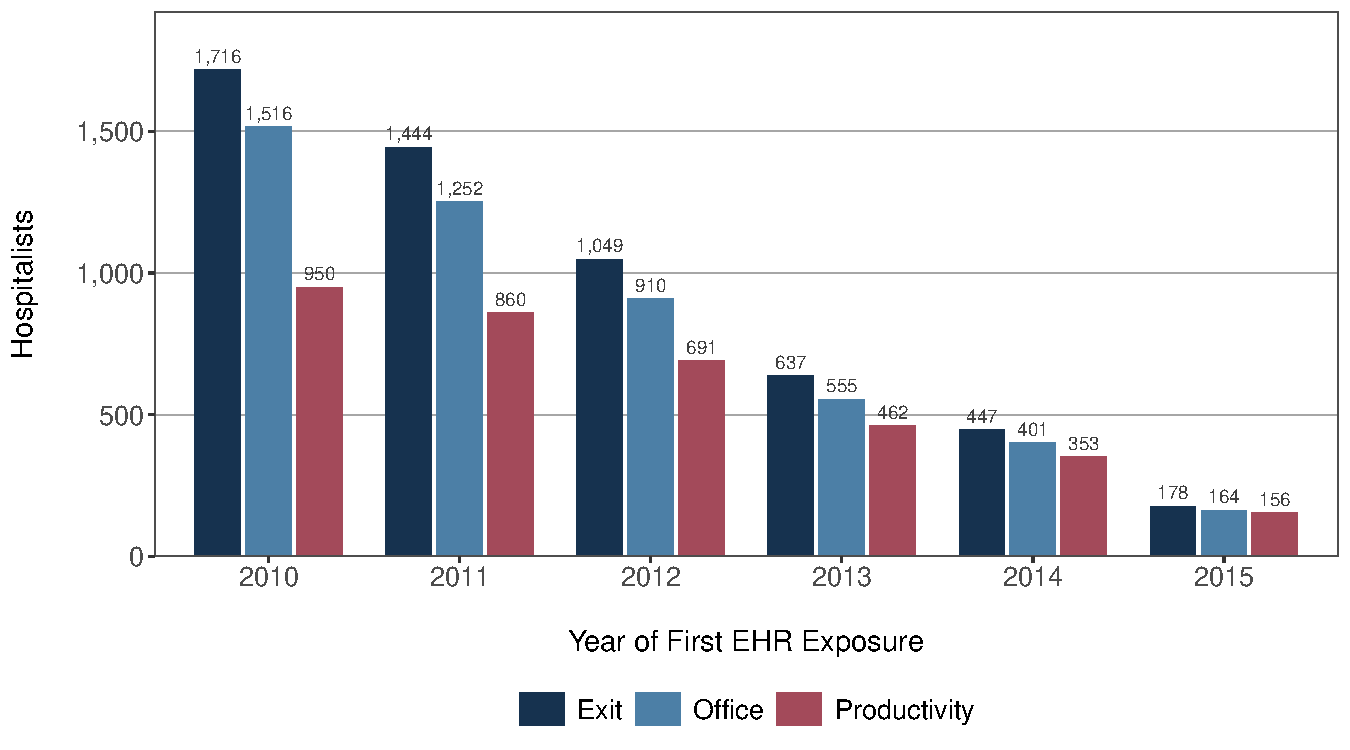
\includegraphics[width=.9\linewidth]{Objects/cohort_sizes.pdf}
    \label{fig:cohortsizes}
    \caption*{\footnotesize \textit{Notes:} Bars show the number of hospitalists first exposed to an EHR in each year, 2010–2015, separately for each estimation sample. The Exit sample includes all hospitalists in the final sample and is used to estimate effects on exit from clinical practice. The Office sample excludes hospitalists who exit clinical practice during the sample period and is used to estimate effects on work setting. The Productivity sample further excludes hospitalists who shift more than 30\% of their patients to an office setting and is used to estimate effects on patient volume and claims per patient. Hospitalists exposed in 2009, the first year of the sample, are excluded from all samples. Sample construction is described in Section \ref{sec:sample}.}
\end{figure}


\subsection{Dependent Variable Construction}

All dependent variables are built based on the MD-PPAS physician-level data set described in Section \ref{sec:sample}. The first dependent variable I consider is the decision for a hospitalist to stop seeing patients, which I refer to as exit. Exit is an indicator variable equal to one in the first year that a hospitalist has no patients recorded in any future year. This indicator variable turns on in the year of exit and remains one in every year after, so it is a cumulative measure of exit. 

The next set of variables I construct capture hospitalist's work setting. The primary variables focus on the physical place of work: the fraction of claims in an office, and an indicator variable equal to one if a physician has any positive claims in an office. To investigate mechanisms for switching office setting, I utilize indicator variables for each physician's associated organization, described in Section \ref{sec:sample}: hospital-affiliated, staffing company, or independent practice.

Finally, I consider outcome variables which explore care/billing patterns, the number of patients seen and claims filed per patient. The number of unique patients captures beneficiaries seen by the physician in any setting, so it reflects a physician's total patient volume rather than volume in a specific setting.\footnote{It would be preferable to examine patient volume in inpatient and outpatient settings separately, particularly given the office-based reallocation documented in Section~\ref{sec:office}. However, constructing setting-specific patient counts in MD-PPAS requires apportioning total claims across settings using the place-of-service
shares described above, which is problematic here because those shares could be correlated with EHR use in the hospital.} Claims filed per patient simply divides a physician's total number of claims by the number of unique patients seen.


\subsection{Summary Statistics}\label{sec:sumstats}

I show summary statistics of relevant variables for each sample in Table \ref{tab:tab:sumstatsnew}. As in the estimation, all always-treated units are dropped from the sample. I follow a maximum of 5,471 eventually-treated hospitalists over time, where the number of hospitalists reduces each time the sample is restricted. The hospitalists in the sample are approximately 46 years old and around a third of the sample are female. A positive number of hospitalists are exposed to an EHR in each year, shown in Figure \ref{fig:cohortsizes}. Out of all hospitalists in the sample, 12\% stop seeing patients at some point. I show a geographic distribution of exiters in Figure \ref{fig:retire_dist}, which shows that exiting occurs across the country. For hospitalists in the office setting sample (those who do not exit), 30\% of have a positive number of patients seen in an office, and the average hospitalist files 9\% of their claims in an office setting. Hospitalists who do not exit or switch work setting see 343 patients and file 3.5 claims per patient on average. Consistent across all samples, hospitalists tend to work in 1.2 hospitals and 1.1 systems. 

Employer arrangements in the baseline year, 2009, vary substantially across hospitalists. Approximately half of hospitalists in the office sample are affiliated with a hospital or integrated health system, while 18\% primarily receive payment through staffing companies and 5\% are classified as solo or independent practitioners. The presence of solo or independent physicians in the beginning of the sample reflects the distinction between employment status and practice location. Physicians may operate independently while still delivering the majority of their services in hospital settings through contractual relationships with hospitals, though this is more rare than using a staffing company. In Table \ref{tab:means_age}, I also show means of these variable by subgroup: hospitalists above and below 60 years of age. 

\import{Table Code}{overall_stats_new.tex}







\section{Empirical Strategy}\label{sec:empstrat}

Since the underlying characteristics of hospitals with different adoption timing may be correlated with the decision to adopt, treatment effects may be heterogeneous across hospitalists who are exposed in different years. Therefore, to avoid negative weighting issues this causes in a classical two way fixed effects specification, I estimate average treatment effects for a specific group $g$ at time $t$: 
$$ATT(g,t)=\mathbbm{E}[Y_t(g)-Y_t(0)|G_g=1],$$
where $G_g=1$ for those in group $g$. A group indicates all hospitalists treated, or first exposed to an EHR, in the same year. I employ the doubly robust estimator established in \citeauthor{sant2020doubly} (\citeyear{sant2020doubly}), without additional covariates, and use not-yet-treated hospitalists as the comparison group. All event-time estimates are measured relative to a universal base period, the year before first EHR exposure (event time $-1$). I aggregate the group-time estimates to a more familiar event study plot with pointwise 95\% confidence intervals. To summarize each outcome with a single number, I report the overall $ATT$, the average of the post-treatment event-time effects from event time 0 to 4; these values are reported in Table~\ref{tab:main_results} and in the notes to each figure.

Because EHR adoption occurs at the hospital level, hospitalists exposed to the same hospital's adoption may share unobserved shocks, and standard practice would be to cluster at the hospital level. In this setting, however, each physician's exposure year is defined by the first adoption among all of their affiliated hospitals, and a nontrivial share of physicians are linked to more than one adopting hospital in their exposure year. There is therefore often no single hospital to which a physician's treatment timing can be attributed, and any hospital-level cluster depends on a discretionary assignment rule. I instead present the main results with standard errors clustered at the physician level, the level at which treatment timing is defined. Appendix \ref{sec:cluster_robustness} reports results with standard errors clustered by the hospital most likely to be responsible for each physician's EHR exposure. As a robustness check, I also present average treatment effects using stacked difference-in-differences (\cite{cengiz2019effect}) and two-stage difference-in-differences (\cite{gardner2021two}) in Appendix \ref{app:estimators}, which yield qualitatively similar results. For comparison, I also present traditional two-way fixed effects estimates, which tend to be biased towards zero.

For each outcome, I present aggregated group time treatment effects for the full sample of hospitalists, as well as split samples for those at least 60 (typical retirement age) and less than 60 years of age.\footnote{Alternatively, one could estimate the effect for more age groups and observe the relationship between the overall ATT and age. However, the data does not support further sub-setting as sample sizes become small.} The sub-samples are constructed based on maximum age throughout the sample, and thus remain fixed for each year. In the main text, I restrict all figures to a symmetric event-time window of -4 to +4. Because the data begin in 2009, the -5 coefficient is identified only from hospitalists first exposed in 2014 or 2015, a small fraction of the sample, and is correspondingly imprecise. I report it, along with the full set of estimable event-time coefficients, in Appendix \ref{sec:eventstudyestimates}. Because different event times are identified from different sets of cohorts, I also re-estimate each outcome using only the 2012–2014 cohorts, for which a full window from -3 to +3 is observed for every physician. These estimates are smaller in magnitude but retain the same sign (Appendix \ref{sec:balanced}).

\subsection{Identification Assumptions}

There are several standard assumptions in a difference-in-differences estimation necessary to identify the parameters of interest, $ATT(g,t)$. First, I assume a version of parallel trends based on not-yet-treated units: average outcomes for those treated in group $g$ would have followed a parallel trend to those in groups treated in later periods. While this assumption cannot be tested directly, I present p-values for a Wald test of pre-trends for each specification. I also investigate pre-trends by allowing for specified violations in the parallel trends assumption (\cite{rambachan2019honest}), bounding the treatment effect under the restriction that any post-treatment violation is at most $\bar{M}$ times the largest violation observed before treatment. I report the largest $\bar{M}$ for which each effect remains statistically significant. Second, I assume that treatment is not reversed. That is, once a hospitalist is exposed to an EHR, they cannot be un-exposed. For hospitalists that do not switch hospitals, an EHR is a costly technology, so a hospital does not have incentive to un-implement an EHR. Any hospitalists who stop using EHRs through exiting or changing work settings are removed from the relevant sample, satisfying this assumption. Third, I assume hospitalists do not anticipate EHR exposure prior to adoption. Generally, even a complex EHR system can be completely set up within a year, and most systems take 6 to 9 months (\cite{uzialko_2021}). Therefore, I proceed in the main specification under no anticipation. However, I explore and present results for a one-year anticipation period in the specification charts in Appendix~\ref{sec:changes}; while most findings are not drastically changed by this choice, the patient-volume estimate is more sensitive to anticipation than the other outcomes.

To interpret these estimators as the causal effect of EHR exposure, additional institutional assumptions are necessary. First, I assume that when a hospital adopts an EHR, hospitalists working in that hospital are direct users of the technology. While some hospitalists may develop work-arounds to ease the burden of EHR use, it is inevitable that they must interact with the technology in some capacity. The definition of EHR adoption captures physician-facing applications, increasing the likelihood of direct exposure to hospitalists. Second, I assume that EHR exposure is exogenous to hospitalists. That is, hospitalists do not influence the hospital's decision to adopt an EHR, and that adoption is not correlated with other contemporaneous changes to the hospital work environment that could independently affect physician behavior. I provide support for this assumption in Appendix \ref{sec:hospanalysis}, where I show that observable hospital behaviors are not systematically associated with EHR adoption. Finally, my identification strategy requires that inpatient EHR adoption not be confounded with ambulatory EHR adoption, since the HITECH Act incentivized both settings simultaneously. In Appendix~\ref{sec:ambulatory_timing}, I show that inpatient adoption preceded ambulatory adoption, particularly in the early years of the sample when most identifying adoption events occur; that ambulatory systems remained functionally narrower even where adopted; and that under standard assumptions about forward-looking behavior, any remaining correlation in adoption timing would tend to attenuate rather than inflate the estimated effects on office-based work.

\section{Effect of EHR Exposure on Labor Market Outcomes}\label{sec:results}

In Table~\ref{tab:main_results}, I summarize the overall ATT for each outcome, for the full sample and by age group, alongside the pre-treatment mean. EHR exposure increases exit from clinical practice, with the effect concentrated among hospitalists aged 60 and older. Among those who remain in practice, exposure increases both the likelihood of working in an office and the share of claims delivered there. Among hospitalists who remain in inpatient practice, exposure modestly increases patient volume, an effect driven by hospitalists under 60. I discuss each outcome, its event-study estimates, and its robustness in turn below.

\begin{table}[htbp]
\centering
\small
\caption{Effect of EHR Exposure on Hospitalist Outcomes: Overall ATT Estimates}
\label{tab:main_results}
\begin{tabular*}{\linewidth}{@{\extracolsep{\fill}} l c c c c}
\toprule
 & Pre-treatment & \multicolumn{3}{c}{ATT (SE)} \\
\cmidrule{3-5}
Outcome & mean & All & Age $<$ 60 & Age $\geq$ 60 \\
\midrule
\multicolumn{5}{l}{\textit{Panel A: Exit}} \\
Exit clinical practice & 0.084 & 0.013 (0.007) & 0.007 (0.008) & 0.043 (0.020) \\
\addlinespace
\multicolumn{5}{l}{\textit{Panel B: Office}} \\
Works in an office & 0.279 & 0.115 (0.016) & 0.099 (0.017) & 0.177 (0.042) \\
Fraction of claims in office & 0.033 & 0.111 (0.008) & 0.100 (0.008) & 0.158 (0.026) \\
\addlinespace
\multicolumn{5}{l}{\textit{Panel C: Productivity}} \\
Number of patients & 336 & 18.5 (7.6) & 20.5 (8.4) & $-$0.03 (20.7) \\
Claims per patient & 3.54 & $-$0.246 (0.096) & $-$0.232 (0.084) & $-$0.372 (0.523) \\
\bottomrule
\end{tabular*}

\vspace{0.5em}
\begin{minipage}{\linewidth}
\footnotesize
\textit{Notes:} Each estimate is the overall average treatment effect on the treated (ATT), estimated following Callaway and Sant'Anna (2021) with not-yet-exposed hospitalists as the comparison group. Bootstrapped standard errors clustered at the physician level are in parentheses. Age groups are defined by maximum age over the sample period. Pre-treatment mean is the mean of the outcome among treated hospitalists at event time $-1$. Because exit is measured cumulatively, the mean reported for exit is the counterfactual mean at event time 4.
\end{minipage}
\end{table}


\subsection{No Longer Seeing Patients}\label{sec:retire}

 The estimates in Figure \ref{fig:retire} represent the effect of EHR exposure on the probability of having exited practice by that event time.\footnote{Appendix Table \ref{tab:ci_retired_ever} reports the point estimates and confidence intervals underlying Figure \ref{fig:retire}.} Estimates for the entire sample of hospitalists are shown in Figure \ref{fig:retirefirst}. The effect is numerically modest but statistically significant: EHR exposure increases the probability of having exited 1-3 years after exposure by up to 2.5 percentage points. Relative to a counterfactual cumulative exit rate of roughly eight percent, EHR exposure increases the probability of leaving practice within four years by 31\%. Because the outcome is cumulative, the rising path of coefficients through year three reflects the continued accrual of exits, not necessarily larger increases over time. A clear difference emerges when the estimation is split by age group, shown in Figure \ref{fig:retiresecond}. Though noisy, the level effect is larger for hospitalists over 60 in every year after exposure, reaching seven percentage points by year four, compared with two percentage points and only marginal statistical significance for those under 60 by year three. Relative to counterfactual four-year exit rates of 7.4 and 11.7 percent, EHR exposure raises cumulative exit by roughly 27\% among hospitalists under 60 and roughly 60\% among those over 60. Therefore, the effect intensifies for older users.

\begin{figure}[ht!]
\centering
    \captionsetup{width=.85\linewidth}
    \caption{Effect of EHR Exposure on No Longer Seeing Patients}
   \begin{subfigure}[]{.9\textwidth}
   \centering
   \caption{Full Sample}
   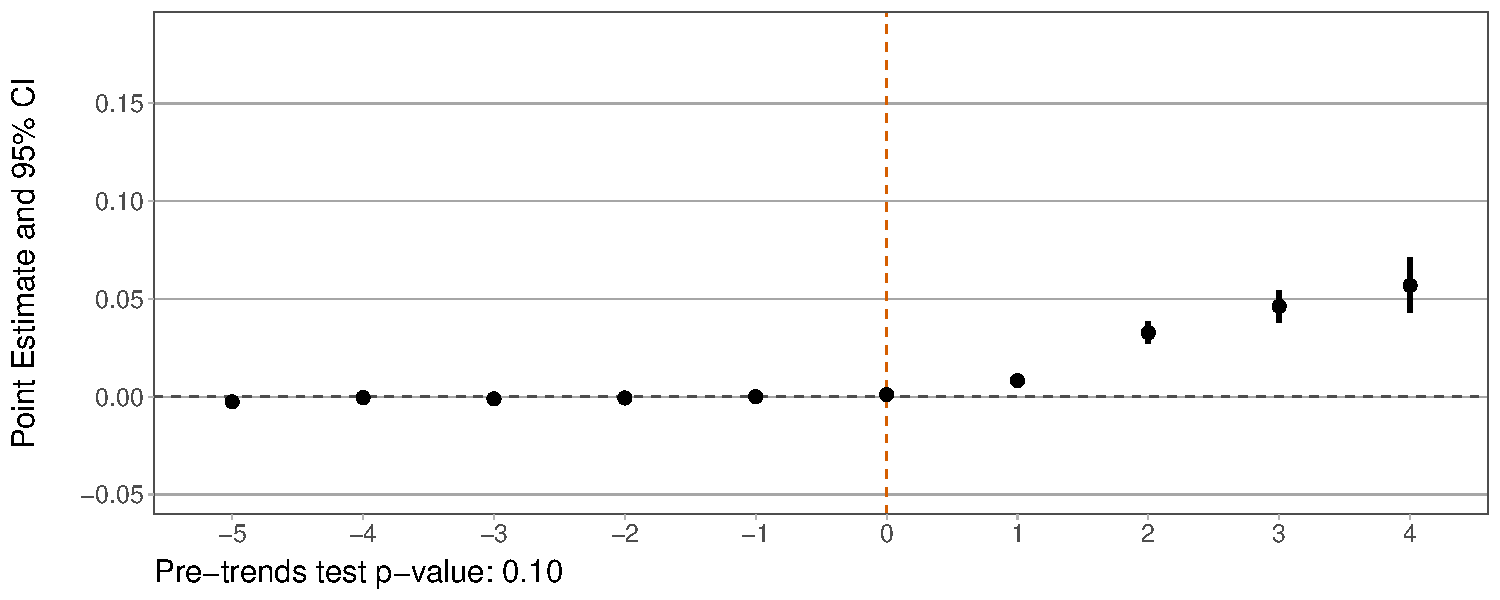
\includegraphics[width = 0.9\textwidth]{Objects/retire_plot_all_new.pdf}
   \label{fig:retirefirst} 
\end{subfigure}

\vspace{1.5mm}

\begin{subfigure}[]{.9\textwidth}
\centering
\caption{Heterogeneity by Age}
   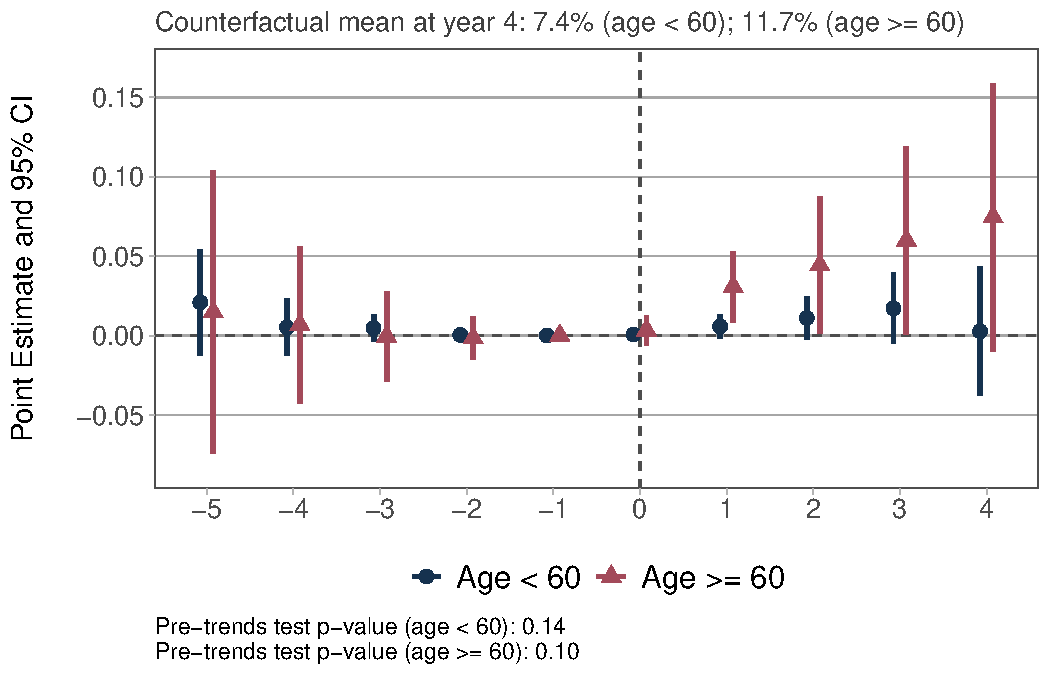
\includegraphics[width = 0.9\textwidth]{Objects/retire_plot_ages_new.pdf}
   \label{fig:retiresecond}
\end{subfigure}
\label{fig:retire}
\vspace{2mm}
    \caption*{\footnotesize{\textit{Notes:} Panel (a) shows average group time treatment effects aggregated over groups to an event study plot. Panel (b) shows these results for different subgroups of physicians by age. The p-value listed for each graph corresponds to a Wald test for pre-trends. Confidence intervals shown are pointwise 95\% intervals. ATT for all, $<$ 60, $>=$ 60 with SE in parentheses: 0.013 (0.007), 0.007 (0.008), 0.043 (0.020), respectively. Counterfactual mean is the realized mean among treated hospitalists at event time four, less the estimated ATT.}}
\end{figure}

The evidence on parallel trends is mixed. For the full sample, the joint Wald test rejects the null at conventional levels. The tests do not reject for either age subgroup $(p=0.14$ and $p=0.10)$, though this partly reflects the reduced precision that comes from splitting the sample rather than cleaner pre-trends. These tests should be interpreted with caution in any case: exit from clinical practice is rare and more concentrated in the final years of the panel, so pre-treatment cohort-years contain few exits and the tests have limited power. Additionally, the estimated effect remains statistically significant only for $\bar{M}$ below 0.25 (Table \ref{tab:honest_breakdown}). However, the benchmark is small: pre-treatment violations reach at most 0.0035, so $\bar{M} = 0.25$ corresponds to a permitted violation of under one tenth of a percentage point. I also estimate the effect of EHR exposure on exit under 36 different specification adjustments, shown in Figure \ref{fig:retire_chart}. While the magnitude remains non-negative under all changes, there is a lack of precision across the board. I therefore read the exit results as suggestive rather than definitive: the evidence points toward EHR exposure accelerating departure from clinical practice, particularly for those of retirement age, but the magnitude should be interpreted with caution.


\subsection{Work Setting}\label{sec:office}

This section reports whether hospitalists shift work to an office setting after EHR exposure in their affiliated hospital. I consider both the extensive margin of working in an office and the intensive margin of the fraction of claims filed in an office. Shown in Figure \ref{fig:officefirsta}, for the full sample of hospitalists, EHR exposure increases the likelihood of working in an office by at least five percentage points in every year after being exposed, where the effect continues to increase over time up to 15 percentage points in year four. Relative to a pre-treatment mean of 28\%, this represents an approximately 50\% increase relative to the mean. The persistence of this effect through four years after exposure suggests a lasting shift in practice setting rather than only a short-run response to implementation costs.\footnote{Appendix Table \ref{tab:ci_work_in_office} reports the underlying estimates and interval widths.} To continue investigating how different age groups may respond differently to technology, I also present estimates for hospitalists less than 60 and greater than or equal to 60 separately in Figure \ref{fig:officefirstb}. While the confidence intervals overlap, the estimate magnitudes are larger in each post-year for those above 60, rising from eight percentage points in event year zero to 25 percentage points in event year four. However, the proportion of hospitalists working in an office pre-exposure is also greater for those above 60, so relative to the average the results are similar.

\begin{figure}[ht!]
\centering
    \captionsetup{width=.9\linewidth}
    \caption{Effect of EHR Exposure on Working in Office Indicator}
   \begin{subfigure}[]{.9\textwidth}
   \centering
   \caption{Full Sample}
   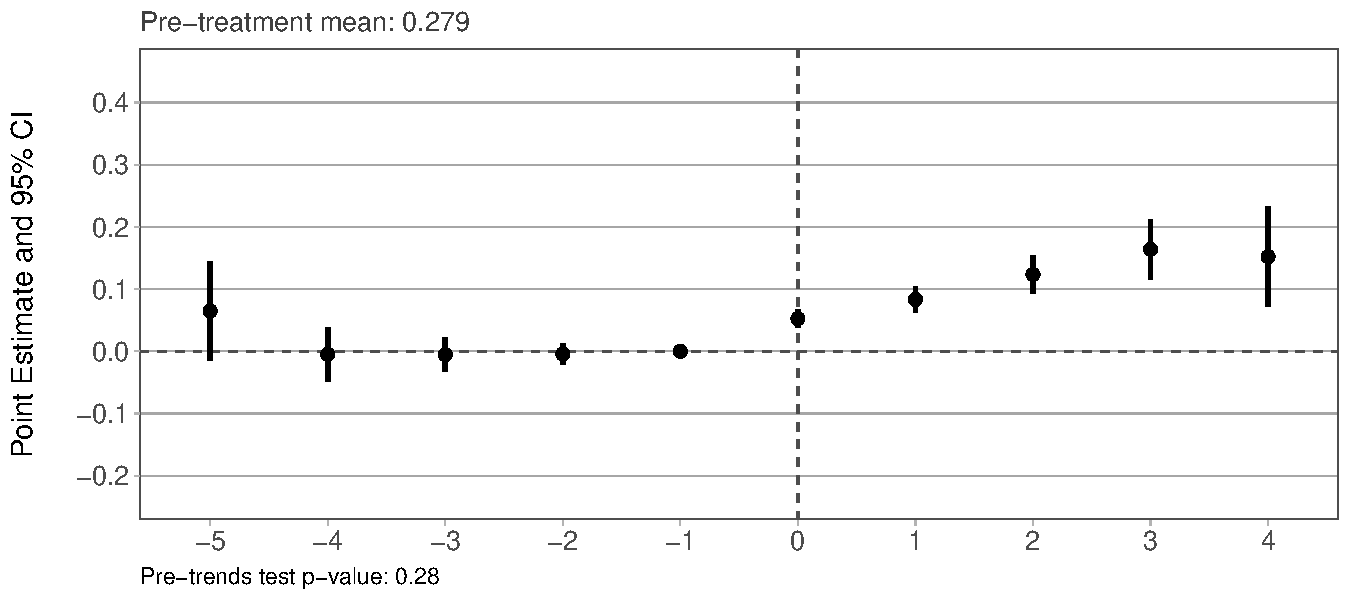
\includegraphics[width=0.9\textwidth]{Objects/officeind_plot_all_new.pdf}
   \label{fig:officefirsta} 
\end{subfigure}

\vspace{3mm}

\begin{subfigure}[]{.9\textwidth}
\caption{Heterogeneity by Age}
\centering
   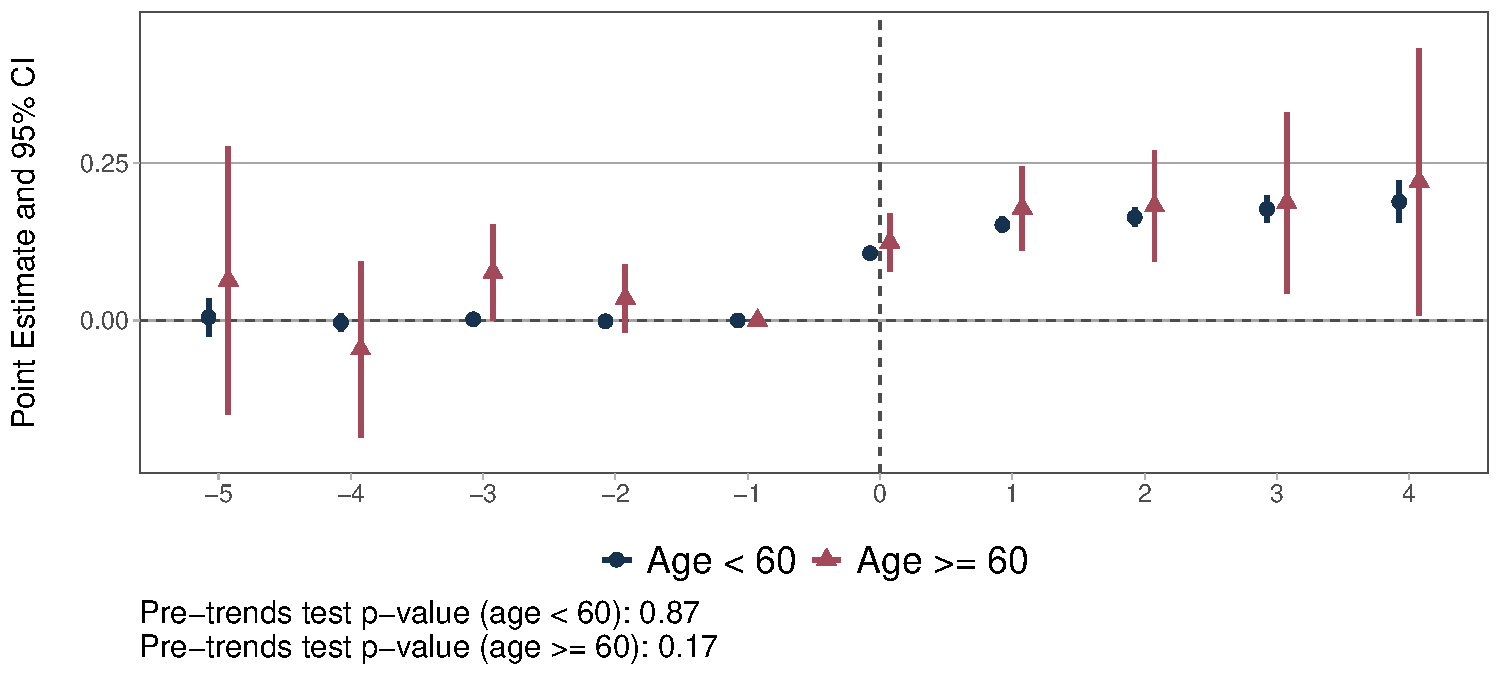
\includegraphics[width=0.9\textwidth]{Objects/officeind_plot_ages_new.pdf}
   \label{fig:officefirstb}
\end{subfigure}
\label{fig:officefirst}
\vspace{2mm}
    \caption*{\footnotesize{\textit{Notes:} The top panel shows average group time treatment effects aggregated over groups to an event study plot. The bottom show these results for different subgroups of physicians by age. The p-value listed for each graph corresponds to a Wald test for pre-trends. Confidence intervals shown are pointwise 95\% intervals. Overall ATT for all, $<$ 60, $>=$ 60 with SE in parentheses: 0.115 (0.016), 0.099 (0.017), 0.177 (0.042), respectively. Pre-treatment mean is the mean of the outcome among treated hospitalists at event time -1, the year immediately preceding first EHR exposure.}}
\end{figure}


 Pre-treatment coefficients are small and statistically indistinguishable from zero across both panels, and the joint Wald test does not reject the null of parallel pre-trends for the full sample $(p=0.28)$ or for either age subgroup $(p=0.73$ and $p=0.13)$. Table \ref{tab:honest_breakdown} shows the estimated effect remains significantly positive for $\bar{M}$ greater than two.  Additionally, Figure~\ref{fig:work_chart} shows estimates under 36 specification adjustments to assess robustness to subjective data choices. The average treatment effect range from 0.05 to 0.14 and remains statistically significant under every combination. 

EHR exposure does not only change the extensive decision of work setting, but also increases the share of claims filed in an office setting, shown in Figure \ref{fig:officesecond}.\footnote{I report the underlying estimates and intervals in Appendix Table \ref{tab:ci_pos_office}.} For the full sample (Figure \ref{fig:officeseconda}) the estimated effect rises from roughly four percentage points in the year of exposure to approximately 17 percentage points by year four. Because the pre-treatment mean is very low at three percent, this represents a substantial shift in where clinical work takes place. Splitting by age, shown in Figure \ref{fig:officesecondb}, the pattern shown for the extensive margin extends to this outcome. Hospitalists over 60 increase their share of work in an office more than those under 60 in terms of levels, but the results are similar when comparing to the pre-exposure mean. 



\begin{figure}[ht!]
\centering
    \captionsetup{width=.9\linewidth}
    \caption{Effect of EHR Exposure on Fraction of Claims in Office}
   \begin{subfigure}[]{.9\textwidth}
   \centering
   \caption{Full Sample}
   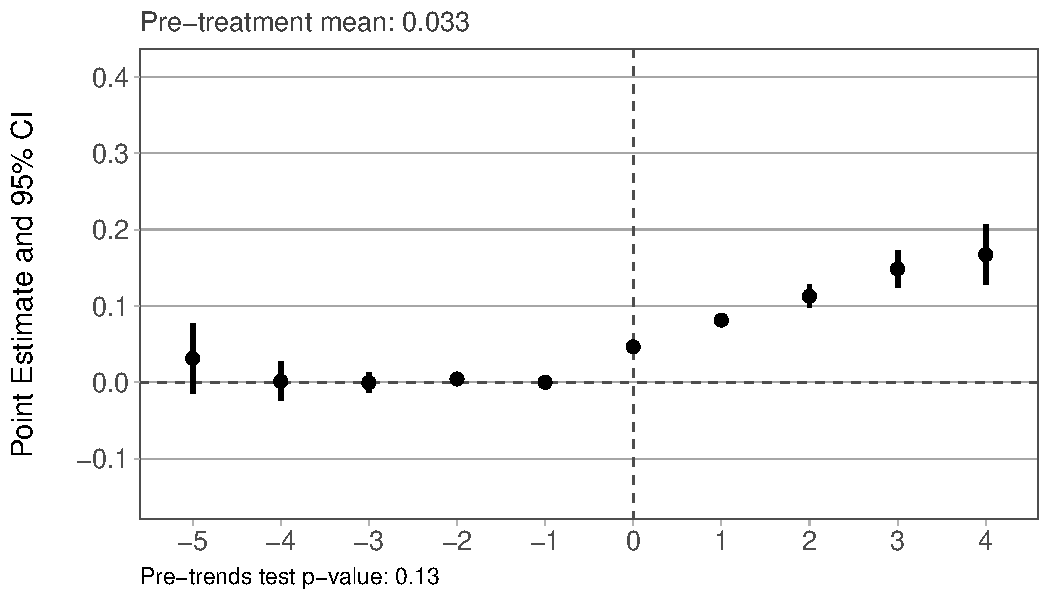
\includegraphics[width=0.9\textwidth]{Objects/officefrac_plot_all_new.pdf}
   \label{fig:officeseconda} 
\end{subfigure}

\vspace{3mm}

\begin{subfigure}[]{.9\textwidth}
\centering
\caption{Heterogeneity by Age}
   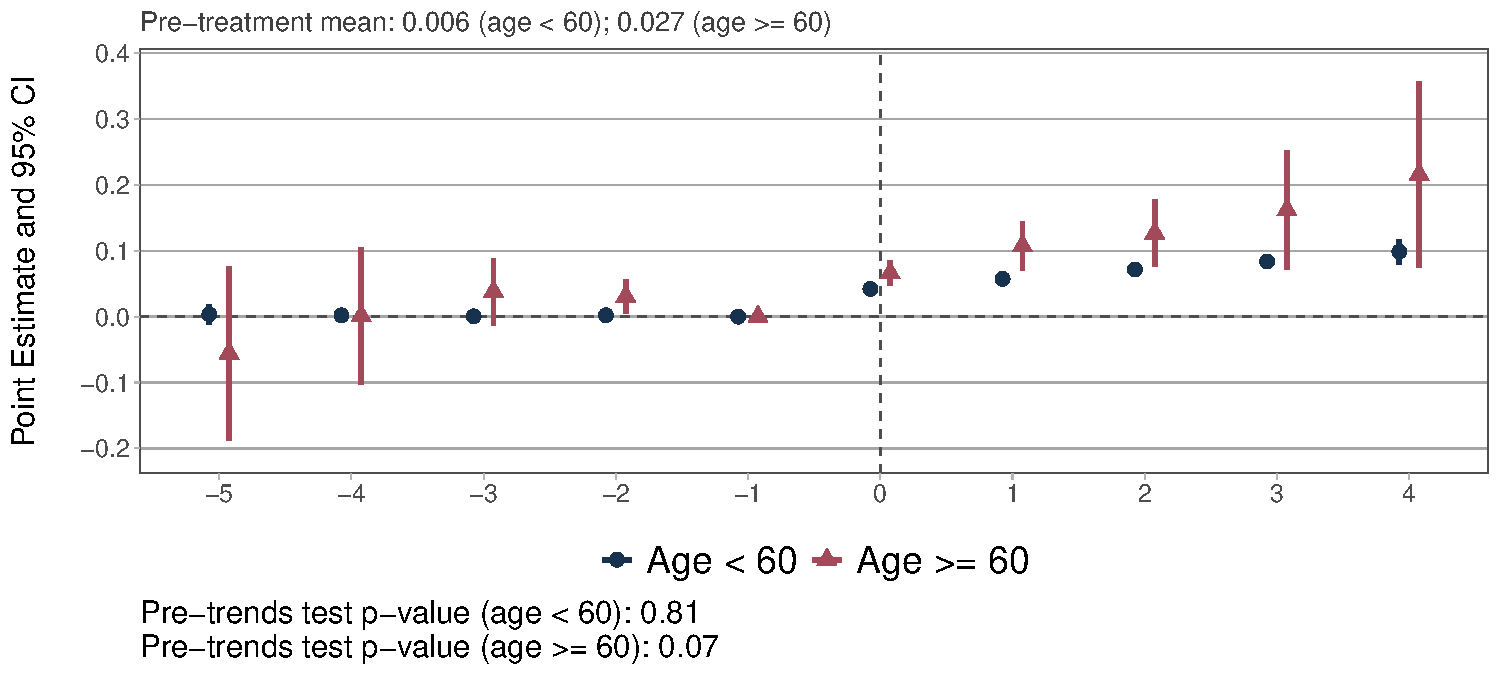
\includegraphics[width=0.9\textwidth]{Objects/officefrac_plot_ages_new.pdf}
   \label{fig:officesecondb}
\end{subfigure}
\label{fig:officesecond}
\vspace{2mm}
    \caption*{\footnotesize{\textit{Notes:} The top panel shows average group time treatment effects aggregated over groups to an event study plot. The bottom show these results for different subgroups of physicians by age. The p-value listed for each graph corresponds to a Wald test for pre-trends. Confidence intervals shown are pointwise 95\% intervals. Overall ATT for all, $<$ 60, $>=$ 60 with SE in parentheses: 0.111 (0.008), 0.100 (0.008), 0.158 (0.026), respectively. Pre-treatment mean is the mean of the outcome among treated hospitalists at event time -1, the year immediately preceding first EHR exposure.}}
\end{figure}

Pre-treatment coefficients are close to zero throughout, and the joint Wald test does not reject the null of parallel pre-trends for the full sample $(p=0.13)$ or for either age subgroup $(p=0.20$ and $p=0.56)$. As with the office indicator, the pre-treatment estimates for hospitalists over 60 have wider confidence intervals, reflecting the smaller size of that subgroup rather than any systematic deviation. This outcome is likewise robust to potential violations of parallel trends and to differing data specifications. As reported in Table \ref{tab:honest_breakdown}, the estimated effect remains significantly positive for $\bar{M}>2$. Figure \ref{fig:fracoffice_chart} shows that under every possible data combination considered, the average treatment effect remains positive and significant, ranging from 0.04 to 0.13. 

Since the sample of hospitalists in the estimation is selected based on never
exiting the sample, which I show in Section~\ref{sec:retire} is correlated with
EHR exposure, the average treatment effect is likely biased. Therefore, I
leverage \citet{lee2009training} bounds. Exposure to
an EHR reduces the share of hospitalists who remain in the sample, so the treated
group I observe is more selected than the comparison group: 87.4 percent of
exposed hospitalists remain, against 90.4 percent of those not yet exposed. For the fraction of patients seen in an office, the bounds run from 0.007 to
0.220, reported in Table \ref{leebouns}. The interval excludes zero, so the finding that EHR exposure shifts
hospitalists toward office-based practice is robust to the selection induced by
exit. I do not report bounds for the indicator for working in an office. Because that outcome takes only two values
and the trimming proportion is small, trimming from either tail removes
observations with identical outcome values, and the upper and lower bounds
coincide. 

\subsubsection{Heterogeneity by Employer Type}

The previous results show that hospitalists shift work away from the inpatient setting following EHR exposure, but leave open the question of what is driving this shift: are hospitalists exercising a preference to work in settings with more autonomy, or are hospitals reallocating their affiliated hospitalists to hospital-owned outpatient facilities? I re-estimate the effect of EHR exposure on the likelihood of working in an office setting separately by hospitalists' baseline employer type, measured in the year prior to EHR exposure.\footnote{I use baseline rather than contemporaneous employer type to avoid conditioning on a post-treatment outcome.} I present these estimates in Figure \ref{fig:office_by_type}.

\begin{figure}[ht!]
\captionsetup{width=.9\linewidth}
    \centering
    \caption{Effect of EHR Exposure on Office Work Indicator by Baseline Employer}
    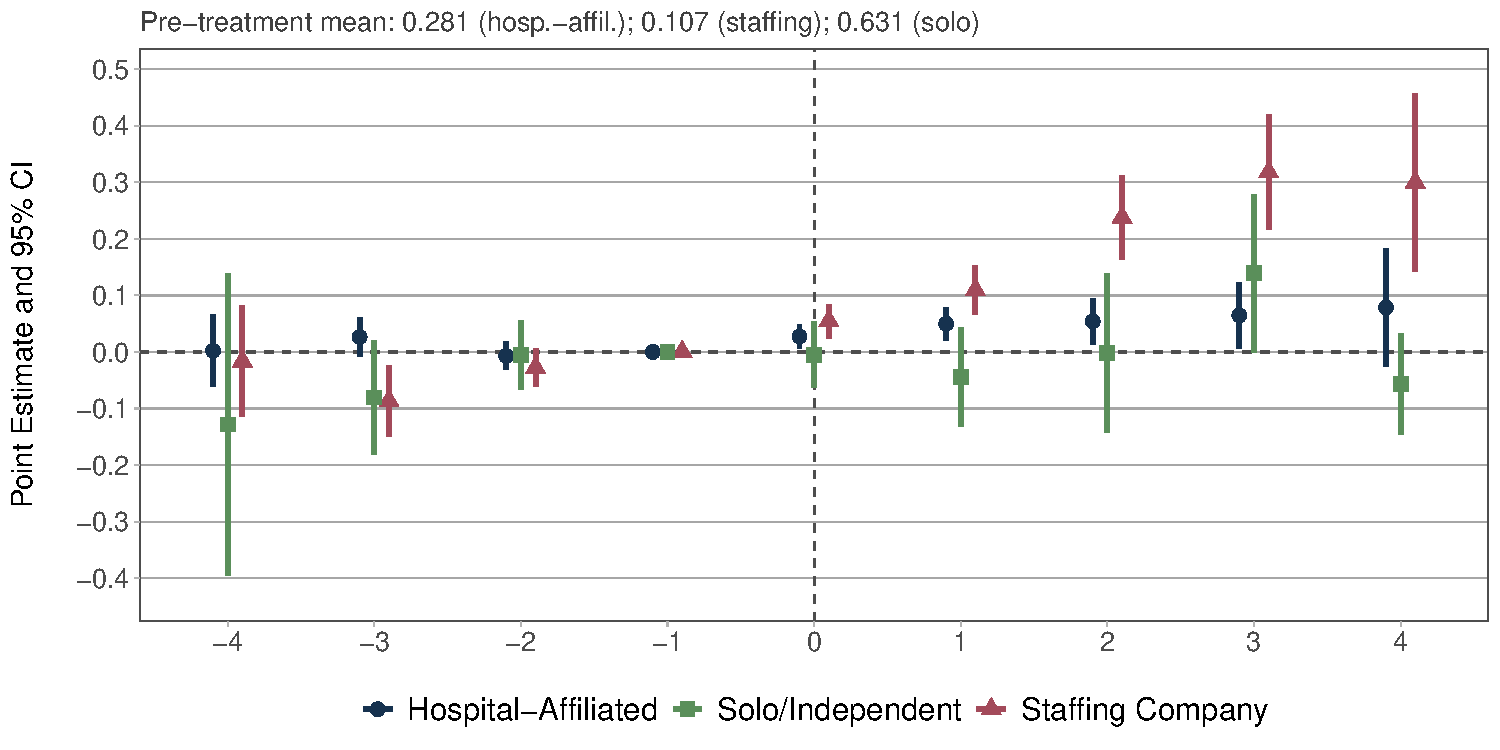
\includegraphics[width=0.85\textwidth]{Objects/work_in_office_by_type.pdf}
    \label{fig:office_by_type}
    \vspace{2mm}
    \caption*{\footnotesize{\textit{Notes:} Plot shows average group-time treatment effects on an indicator for working in an office setting, estimated separately by hospitalists' baseline employer type. Confidence intervals are 95\% and calculated using the estimator of \citeauthor{callaway2021difference} (\citeyear{callaway2021difference}).}}
\end{figure}

Hospitalists with a staffing company employer in the baseline show by far the largest increase in having any office-based work, rising by roughly 30 percentage points from a baseline of 10.7\% by three to four years post-exposure. Hospital-affiliated hospitalists show a smaller but steadily growing increase, from a baseline of 28.1\% to eight percentage points above baseline by year four. Independent hospitalists, who already have a substantially higher baseline rate of office-based work (63.1\%), show little additional movement, consistent with limited remaining room to shift further given their already-high starting point. Pre-trends tests do not reject parallel trends for any of the three groups. Therefore, hospitalists contracted through staffing companies, who supply inpatient coverage as a discrete service rather than holding a long-term employment relationship with a single hospital, are the most responsive to EHR exposure, while hospital-employed hospitalists respond more modestly.

To understand why staffing companies show the largest response, I examine whether hospitalists change their employer type following EHR exposure. I estimate the effect of EHR exposure on a hospitalist's likelihood of having a specific type of entity as their primary employer: hospitals, hospitalist staffing companies, or independent practices, limiting this analysis to hospitalists who reallocated some of their work to an office setting.\footnote{The results hold without this limitation, though the baseline means and point estimates are dampened by those who do not reallocate at all.} Because this restriction conditions on a post-exposure outcome, I interpret these estimates descriptively. I present the results in Figure~\ref{fig:employer_type}. Among hospitalists who reallocate their work, reallocation is accompanied by a shift away from affiliation with a staffing company. The share primarily affiliated with a staffing company, 20.7\% at baseline, declines in every year after exposure relative to the counterfactual, by up to roughly 50 percentage points in year four. The share in solo or independent practice, 2.4\% at baseline, rises by 2.5--7.5 percentage points in each year following exposure. The share affiliated with a hospital also rises, though the confidence intervals include zero at every horizon. Movement into independent practice is difficult to reconcile with hospitals redeploying their own physicians, whereas movement toward hospital affiliation is consistent with either explanation. Taken together with the larger office-based response among staffing-company hospitalists, these results are more consistent with hospitalists responding to EHR-related burden than with hospital reallocation alone, although both mechanisms may operate.

\begin{figure}[ht!]
    \centering
    \captionsetup{width=.9\linewidth}
    \caption{Effect of EHR Exposure on Employer Type Indicators}
    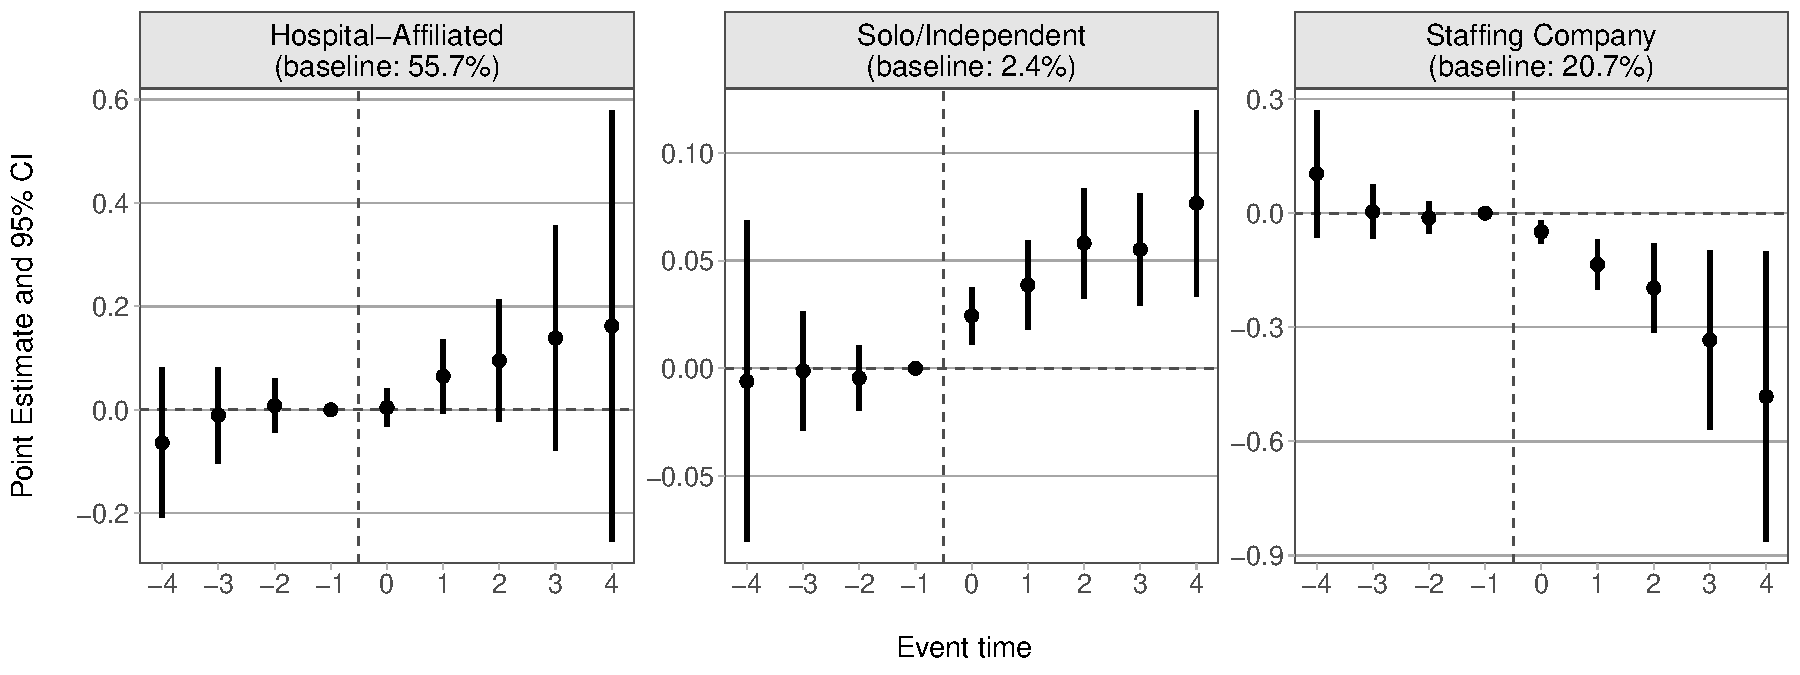
\includegraphics[width=\textwidth]{Objects/employer_types_shifters_eventstudy_appendix.pdf}
    \label{fig:employer_type}
    \caption*{\footnotesize{\textit{Notes:} Plot shows average group-time treatment effects on an indicator for primary affiliation with each employer type, restricted to hospitalists who reallocate some work to an office setting. Baseline shares for each group are reported in the panel subtitles. Confidence intervals are 95\% and calculated using the estimator of \citeauthor{callaway2021difference} (\citeyear{callaway2021difference}).}}
\end{figure}







\subsection{Patient Count and Billing Activity}\label{sec:patientcount}

I now estimate the effect of EHR exposure on patient count and billing activity per patient, shown in Figure \ref{fig:patient}.\footnote{The estimates and confidence intervals underlying these figures are shown in Appendix Table \ref{tab:ci_npi_unq_benes}.} For any age hospitalist (Figure \ref{fig:patienta}), patient count increases in each year after EHR exposure from approximately four patients in year zero to 30 patients in year four after exposure. These estimates translate to a 1-9\% increase in the number of patients seen relative to the mean of 336 patients in the pre-treatment year. These estimates should be read as lower bounds, since MD-PPAS captures only traditional fee-for-service Medicare patients, so any increase in volume among patients with other coverage is not observed. 

\begin{figure}[ht!]
\centering
    \captionsetup{width=.9\linewidth}
    \caption{Effect of EHR Exposure on Number of Patients Seen}
   \begin{subfigure}[]{.9\textwidth}
   \centering
   \caption{Full Sample}
   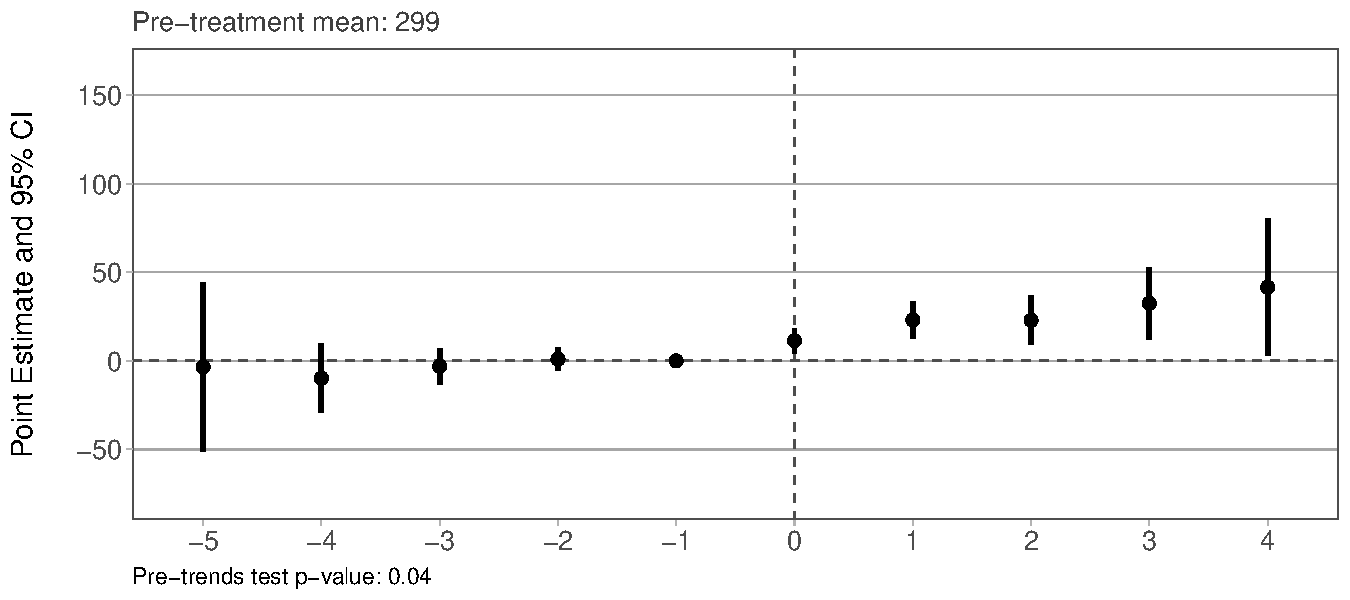
\includegraphics[width=0.9\textwidth]{Objects/patient_plot_all_new.pdf}
   \label{fig:patienta} 
\end{subfigure}

\vspace{3mm}

\begin{subfigure}[]{0.9\textwidth}
\centering
\caption{Heterogeneity by Age}
   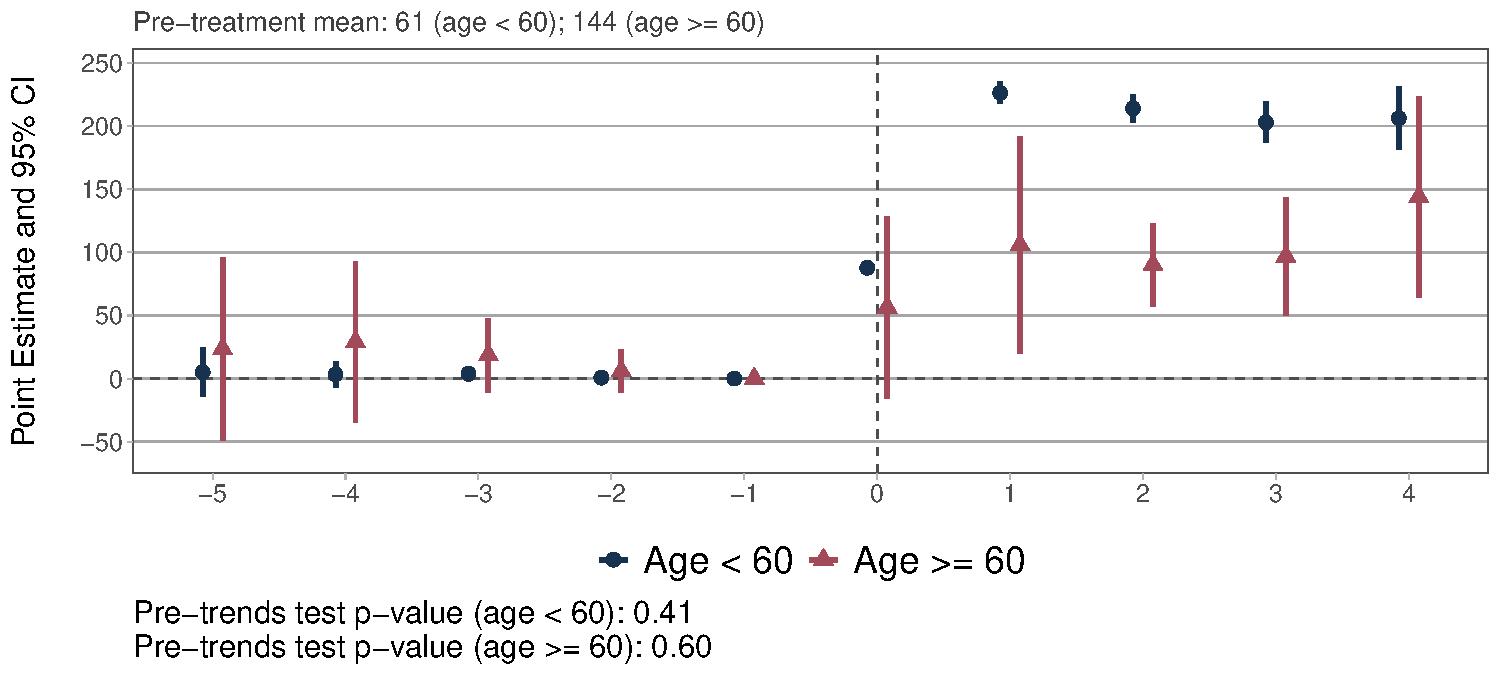
\includegraphics[width=0.9\textwidth]{Objects/patient_plot_ages_new.pdf}
   \label{fig:patientb}
\end{subfigure}
\label{fig:patient}
\vspace{2mm}
    \caption*{\footnotesize{\textit{Notes:} The top panel shows average group time treatment effects aggregated over groups to an event study plot. The bottom show these results for different subgroups of physicians by age. The p-value listed for each graph corresponds to a Wald test for pre-trends. Confidence intervals shown are pointwise 95\% intervals. Overall ATT for all, $<$ 60, $>=$ 60 with SE in parentheses: 18.5 (7.6), 20.5 (8.4), -0.03 (20.7), respectively. Pre-treatment mean is the mean of the outcome among treated hospitalists at event time -1, the year immediately preceding first EHR exposure.}}
\end{figure}

Splitting by age, Figure~\ref{fig:patientb} shows that the increase is concentrated among hospitalists under 60, whose point estimates rise from about four additional patients in the year of exposure to about 40 by year four, with an overall ATT of 20.5 patients. For hospitalists aged 60 and older, the estimates are small and imprecise: the confidence intervals include zero at every horizon, the point estimate turns negative in year four, and the overall ATT is essentially zero. The two groups have nearly identical pre-treatment volumes, 336 and 338 patients respectively, so this difference does not reflect a difference in scale. Given the imprecision of the estimates for older hospitalists, the data cannot rule out an effect of similar magnitude in that group, but the evidence of increased patient volume comes from hospitalists under 60.


The joint Wald test rejects the null of parallel pre-trends for hospitalists aged 60 and older ($p = 0.01$), but not for those under 60 ($p = 0.81$) or for the pooled sample ($p = 0.62$). The sensitivity analysis of \citet{rambachan2019honest} reflects this weaker pre-treatment evidence: the estimated effect on patient volume remains significantly positive only for $\bar{M}$ below 0.25, shown in Table~\ref{tab:honest_breakdown}. I also account for non-random selection into this outcome's estimation sample, since only hospitalists who remain in inpatient practice throughout the sample period contribute to the patient-volume estimates. Lee bounds on the average treatment effect, reported in Table~\ref{leebouns}, range from 9.6 to 20.2 patients, confirming that the direction of the estimated effect is robust even under worst-case assumptions about selection into the sample. The estimated effect is also sensitive to the choice of standard error clustering: while significant under the main specification's physician-level clustering, it is not statistically significant when instead clustering by the hospital responsible for a physician's EHR exposure timing ($p = 0.11$; Appendix~\ref{sec:cluster_robustness}). I also assess sensitivity to the choices made in constructing the sample, shown in Appendix Figure~\ref{fig:pat_chart}. The estimates range from null to positive in every specification. The smaller estimates come from specifications permitting one year of anticipation, which reclassify the year before adoption as treated. Because the estimated effects build over event time and are smallest immediately after exposure, including an additional early period in the aggregation mechanically lowers the average. Overall, the sensitivity analyses suggest that EHR adoption had a non-negative effect on patient volume, though the statistical support for a positive effect varies across identification and inference assumptions.

I also consider whether EHR exposure affects claims filed per patient. The post-exposure coefficients are negative and statistically significant (Figure \ref{fig:claima}). However, this outcome provides the strongest evidence of violations in the parallel trends assumption (Table \ref{tab:honest_breakdown}) and is the least robust to changes in data specifications (Figure \ref{fig:cpp_chart}). Therefore, I do not interpret these results as suggesting EHR exposure affects claims per patient. Splitting by age does not change this conclusion.


\subsubsection{Re-allocation of Patients}

It could be possible that any increase in patient count is due to re-allocation of patients after other hospitalists exit as opposed to a true productivity increase. Using the exit estimates from Section \ref{sec:retire}, I calculate the increase in patient volume that would follow if all patients of exiting hospitalists were reassigned to those who remain. Because exit is measured cumulatively, the coefficient at event time $e$ gives the additional share of hospitalists who have left practice by that point. Denoting this share $s_e$, full reassignment implies an increase of $\bar{y} \cdot s_e/(1-s_e)$ patients per remaining hospitalist, where $\bar{y} = 336$ is the pre-treatment mean. Across the post-treatment window, redistribution can explain between 9 and 34 percent of the estimated effect, with the remainder attributable to changes in the practice of hospitalists who do not exit. This calculation is an upper bound on the contribution of redistribution: it assumes that every patient of an exiting hospitalist is reassigned to another hospitalist in the sample, and that hospitals do not replace departing physicians, whereas Table \ref{tab:hosp_outcomes} shows no association between EHR adoption and hospital physician counts. The increase in patients seen therefore does not appear to be an artifact of a shrinking hospitalist workforce.


\subsection{Potential Threats to Validity}\label{sec:alt_main}

I assess four potential threats to validity: (1) other hospital initiatives coinciding with EHR adoption, (2) changes to Medicare policies, (3) changes in claim coding, and (4) EHR adoption in ambulatory facilities.


\subsubsection{Other Hospital Changes}

EHR adoption may coincide with other hospital initiatives to improve productivity or quality. Such changes would likely offset some of the burden imposed by the EHR, making the estimates for exit and work setting lower bounds, but would bias the patient-volume estimates away from zero. To assess this concern, I apply the main estimator to a hospital-level panel of other investments, including capital investment, staffing, and vertical integration with physicians. Although these estimates are not causal, I find no evidence that other investment decisions change alongside EHR adoption (Appendix \ref{sec:hospanalysis}).


\subsubsection{Medicare Policy Changes}

Changes affecting the Medicare population under the Affordable Care Act (ACA) could confound the estimates if they influenced the timing of EHR adoption or the behavior of exposed hospitalists. I find little support for this explanation (Appendix \ref{sec:aca}). Average group-time treatment effects are similar across adoption cohorts, with no discontinuity for hospitals adopting in 2012 or 2014, when major ACA initiatives took effect. Prior evidence finds no effect of Medicaid expansion on Medicare utilization, and no hospitalist in the sample opted out of Medicare, making a shift toward privately insured patients unlikely.


\subsubsection{Changes to Coding Procedure}

The increase in office-based work could reflect hospitalists billing existing inpatient encounters under different codes rather than taking on new office-based patients. Using billing-code data available from 2013, I find that hospital-based billing categories are unchanged following EHR exposure, while the increase is concentrated in visit codes that can only be billed in an office setting (Appendix \ref{app:coding}). This pattern is consistent with hospitalists taking on new office-based patients rather than relabeling inpatient encounters.


\subsubsection{Ambulatory EHR Adoption}

Because the HITECH Act also incentivized EHR adoption in ambulatory settings, the office shift could reflect a reallocation of work toward settings undergoing comparable technological change rather than an escape from EHR burden. Using data on ambulatory EHR adoption (Appendix~\ref{sec:ambulatory_timing}), I show that inpatient adoption preceded ambulatory adoption, particularly in the early years of the sample when most identifying adoption events occur, and that ambulatory systems remained functionally narrower even where adopted. Any remaining correlation in adoption timing would, under standard assumptions about forward-looking behavior, tend to attenuate rather than inflate the estimated effect on office-based work. This argument does not extend to exit, since a hospitalist anticipating ambulatory adoption may choose to leave practice rather than relocate, so part of the exit effect may reflect anticipated EHR exposure beyond the hospital. Taken together, office-based practice likely remained a lower EHR-burden alternative to hospital practice during the period of adjustment.


\section{Conclusion}

The adoption of health information technology was expected to revolutionize the healthcare system in the U.S. by improving efficiency, reducing costs, and enhancing quality of care. However, the anticipated benefits have yet to be fully realized. A critical gap remains in understanding how physicians respond to its implementation. This paper examines the effect of hospital EHR adoption on hospitalists' decisions to leave clinical practice or switch work settings, as well as its effect on the productivity of those who remain in inpatient practice.

I employ a staggered difference-in-differences framework to estimate these effects. I find that hospitalists exposed to EHR adoption are more likely to exit clinical practice altogether, with effects concentrated among physicians aged sixty and older. Among hospitalists who remain in practice, EHR exposure increases the likelihood of shifting work toward office settings; this shift is accompanied by movement out of staffing arrangements and toward independent practice. Among hospitalists who remain in their original setting, I find an increase in patient volume that cannot be fully explained by patient redistribution or selective physician attrition, though this result is the most sensitive to specification choices. I consider several alternative explanations for these findings, including concurrent hospital initiatives, changes affecting the Medicare population under the Affordable Care Act, changes in billing-code composition, and the simultaneous roll-out of ambulatory EHRs. None of these alternatives fully account for the pattern of results, supporting a causal interpretation of EHR exposure as the driver of the labor market responses observed. The office-based results are robust across a wide range of checks, while the exit and patient-volume results are directionally stable but more sensitive to specification and inference choices.

The findings speak to a growing literature on how health information technology affects the physician labor market. \citet{lin2026health} find that health IT diffusion increased hospital-based physician density, with growth concentrated among early-career physicians. The individual-level margins I document offer a complementary labor-supply mechanism: older hospitalists exit following EHR exposure, while patient volume rises among younger hospitalists who remain, consistent with a reallocation of hospital-based labor toward early-career physicians. Relatedly, \citet{greenwood2019does} show that physicians stay longer at their hospital when an EHR complements their work but leave in greater numbers when it disrupts established routines.

This paper shows the importance of accounting for the adjustment costs of new technologies alongside their long-run benefits. Costs that arise during implementation can have lasting effects on where physicians choose to work, and because these costs are not borne evenly, they shape which physicians are positioned to realize a technology's benefits. As policymakers design mandates or incentives for future technology adoption, they should anticipate labor supply responses, particularly from physicians with the least time or attachment to benefit from learning a new system, in addition to changes in physician practice patterns. Although the estimates are identified from the initial wave of EHR adoption between 2009 and 2015, the broader lesson likely extends beyond this specific setting. Many healthcare technologies require physicians to adopt new workflows, learn unfamiliar systems, and absorb substantial short-run adjustment costs. To the extent that these features characterize other technological changes, the labor market responses documented here may generalize to future episodes of technology adoption. As digital technologies continue to expand throughout healthcare, understanding these labor market responses will be increasingly important for predicting the full consequences of technology adoption.




\clearpage
\onehalfspacing

\printbibliography

\clearpage

\normalsize
\appendix

\renewcommand{\thetable}{A\arabic{table}}
\renewcommand{\thefigure}{A\arabic{figure}}

\section{Data}\label{app:data}

This sections outlines in detail the data used throughout the paper. I begin by identifying physician and hospital National Provider Identifier (NPI)\footnote{\hyperlink{https://download.cms.gov/nppes/NPI/Files.html}{\text{https://download.cms.gov/nppes/NPI-Files.html}}}, an identifier of each medical entity, using a description of their tax code\footnote{\hyperlink{https://nucc.org/index.php/code-sets-mainmenu-41/provider-taxonomy-mainmenu-40/pdf-mainmenu-53}{\text{https://nucc.org/index.php/code-sets-mainmenu-41/provider-taxonomy-mainmenu-40/pdf-mainmenu-53}}}. I categorize NPIs by key words: any description containing ``Internal Medicine", ``Hospitalist", ``Family Medicine", or ``General Practice" is classified as a primary care physician (PCP), and any description containing ``hospital" is classified as a hospital. I create two data sets, one containing only PCPs and one containing only hospitals, which are used to identify the relevant NPIs in the Center for Medicare and Medicaid Services (CMS) Shared Patient Data. 

For years 2009-2015, the CMS collected detailed information on the number of Medicare patients shared between any two NPIs within 30, 90, or 180 day intervals.\footnote{\hyperlink{https://www.nber.org/research/data/physician-shared-patient-patterns-data}{https://www.nber.org/research/data/physician-shared-patient-patterns-data}} In this paper, I use the data files that capture shared patient activity in 30 day intervals. I merge the shared patient data to the filtered tax codes to identify NPIs who are either PCPs or hospitals. I limit to pairs including one physician and one hospital. I combine duplicates into one observation, summing the same day count variable. Most of the pairs have very few shared patients, which is not indicative of the physician working inside the hospital. I drop any pairs who do not have at least 30 same-day shared patients.\footnote{I also consider thresholds of 10 and 60. Results are similar and can be found in Figure \ref{sec:changes}.} I combine the physician-hospital pairs with various data sets containing hospital and/or physician level information, which I eventually aggregate to the physician-level.

\subsection{Hospital-Level Variables}\label{sec:hosplevel}

I use an AHA-NPI crosswalk to merge the hospitals in each pair to the Annual Hospital Administration Survey (AHA Survey) from 2009--2017. Further, I use a hospital's Medicare ID number to merge this data to the Healthcare Information and Management Systems Society (HIMSS) data. I draw on these two sources that measure adoption differently but provide a more complete picture of EHR use within a hospital. In the AHA Survey, hospitals are asked to report the status of their electronic health record implementation. The variable \texttt{EHLTH} takes three values: 0 for not implemented, 1 for partially implemented, and 2 for fully implemented. This is a
single self-reported measure covering the institution as a whole. Alternatively, the HIMSS Analytics database records the status of individual clinical applications at each hospital. For each hospital-year, HIMSS reports whether a given application is not automated, not yet contracted, contracted but not installed, in the process of installation, live and operational, or scheduled to be replaced. I code an application as present if its status is ``live and operational''. HIMSS reports at the level of individual entities, several of which may map to a single Medicare provider number. Where this occurs, I code an application as present at the hospital if it is live at any affiliated entity. 

Adoption of these systems was driven substantially by the HITECH Act's Meaningful Use incentive program. Figure~\ref{fig:meanuse} illustrates the geographic expansion of this roll-out, comparing hospitals receiving Stage 1 subsidies in 2011 against those receiving them by 2013.

\begin{figure}[ht!]
    \centering
    \caption{Hospitals Receiving Meaningful Use Stage 1 Subsidy}
    \label{fig:meanuse}
    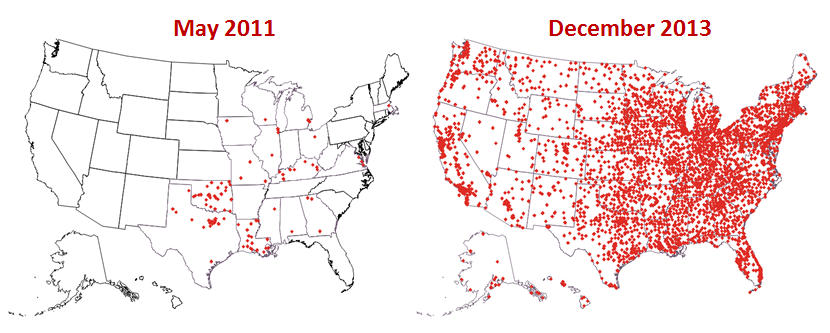
\includegraphics[width=0.9\textwidth]{graphics/QS-Hospitals-Receiving-Payments-for-MU-and-Adoption.png}
    \caption*{\footnotesize \textit{Source:} HealthIT.gov}
\end{figure}

HIMSS classifies a number of applications under the heading of electronic medical records. However, some of these applications are back-end information storage applications that most hospitals employed long before meaningful use standards were established. I distinguish between those physicians directly interact and those that operate as back-end infrastructure. I count three applications as physician-facing: computerized physician order entry, physician documentation, and physician portal. Each requires the physician to enter or retrieve information themselves, and each therefore changes the physician's workflow. I exclude three applications that appear under the same heading but that physicians do not directly use: the clinical data repository, which consolidates records into a single store; order entry, which refers to order communication systems used by clerical and nursing staff rather than physicians; and clinical decision support, which typically operates in the background of other systems rather than as a standalone interface.

I present the share of hospitals with each combination of answers in the AHA and HIMSS data in Table~\ref{tab:ehr_construct}. This shows that the distinction between the two sources is empirically consequential. The three back-end applications are present in 89 to 93 percent of hospital-years in the sample, compared with 49 to 56 percent for the three physician-facing applications. A definition that counted any electronic medical record application would therefore classify as treated a large number of hospital-years in which no physician workflow had changed. Consistent with this, hospital-years in which only back-end applications are present are overwhelmingly reported to AHA as having no electronic health record or only a partial implementation.

\begin{table}[!h]
\centering
\caption{\label{tab:ehr_construct}EHR Source Comparison}
\begin{threeparttable}
\begin{tabular}[t]{lrrc}
\toprule
 & Hospital-years & Share & EHR indicator\\
\midrule
\addlinespace[0.3em]
\multicolumn{4}{l}{\textbf{Panel A: AHA reported status $\times$ HIMSS applications}}\\
\hspace{1em}\quad Full $\times$ Physician-facing app & 8,261 & 29.4\% & $1$\\
\hspace{1em}\quad Full $\times$ No physician-facing app & 794 & 2.8\% & $1$\\
\hspace{1em}\quad Full $\times$ Not covered & 531 & 1.9\% & $1$\\
\hspace{1em}\quad Partial $\times$ Physician-facing app & 5,687 & 20.3\% & $1$\\
\hspace{1em}\quad Partial $\times$ No physician-facing app & 2,778 & 9.9\% & $0$\\
\hspace{1em}\quad Partial $\times$ Not covered & 861 & 3.1\% & $0$\\
\hspace{1em}\quad No EHR $\times$ Physician-facing app & 412 & 1.5\% & $1$\\
\hspace{1em}\quad No EHR $\times$ No physician-facing app & 1,119 & 4.0\% & $0$\\
\hspace{1em}\quad No EHR $\times$ Not covered & 916 & 3.3\% & $0$\\
\hspace{1em}\quad Not reported $\times$ Physician-facing app & 3,349 & 11.9\% & $1$\\
\hspace{1em}\quad Not reported $\times$ No physician-facing app & 2,131 & 7.6\% & Dropped\\
\hspace{1em}\quad Not reported $\times$ Not covered & 1,221 & 4.4\% & Dropped\\
\addlinespace[0.3em]
\multicolumn{4}{l}{\textbf{Panel B: HIMSS applications used to define physician-facing use}}\\
\hspace{1em}\quad Computerized physician order entry & 13,846 & 56.4\% & Counted\\
\hspace{1em}\quad Physician documentation & 12,473 & 50.8\% & Counted\\
\hspace{1em}\quad Physician portal & 12,013 & 49.0\% & Counted\\
\hspace{1em}\quad Clinical data repository & 22,533 & 91.9\% & Not counted\\
\hspace{1em}\quad Order entry (non-physician) & 22,786 & 92.9\% & Not counted\\
\hspace{1em}\quad Clinical decision support & 21,861 & 89.1\% & Not counted\\
\bottomrule
\end{tabular}
\begin{tablenotes}
\item \textit{Note: } Table reports the joint distribution of hospital-year EHR adoption status across the two data sources used to construct EHR exposure. Panel A cross-tabulates each hospital-year's self-reported status in the AHA Survey against whether a physician-facing application (computerized physician order entry, physician documentation, or a physician portal) is live and operational in HIMSS. Panel B reports, for each of the six HIMSS clinical application categories tracked, the share of hospital-years in which that application is live and operational, and whether it is counted toward the physician-facing definition.
\end{tablenotes}
\end{threeparttable}
\end{table}


Among hospital-years in which HIMSS records at least one physician-facing application, fewer than half are reported to AHA as fully implemented. The remainder are reported as partially implemented (20.3 percent of all hospital-years), as having no electronic health record (1.5 percent), or are not reported to AHA at all (11.9 percent). The reverse case is much rarer: only 2.8 percent of hospital-years are reported as fully implemented while HIMSS records no physician-facing application. This pattern is consistent with the two sources capturing different points in the implementation process. HIMSS records an application once it is operating, possibly in only part of the hospital. The AHA category of ``fully implemented'' requires the hospital to judge the institution-wide roll-out complete. A hospital running computerized order entry on some units while continuing to use paper elsewhere would appear as adopting in HIMSS and as partially implemented in AHA, and both would be accurate. Two further features of the disagreement support this interpretation. First, most disagreements resolve within a year or two, with hospitals subsequently reporting full implementation to AHA. Second, the share of conflicting hospital-years falls steadily across the sample period as implementations mature.

Because physicians face the burden of an electronic record once they must use it, rather than once the hospital considers the project complete, I treat positive evidence from either source as indicating adoption. Specifically, a hospital-year is coded as having an electronic health record if either (1) AHA reports full implementation ($\texttt{EHLTH} = 2$), or (2) HIMSS records computerized physician order entry, physician documentation, or a physician portal as live. A hospital-year is coded as having no electronic health record if AHA reports no implementation or partial implementation and HIMSS records no physician-facing application. A hospital-year is dropped if AHA does not report and HIMSS records no physician-facing application, since in that case neither source provides evidence in either direction. Before applying this rule I interpolate the AHA measure within hospitals. Where a
hospital reports the same implementation status in two years and the intervening year is missing, I fill the intervening year with that status. I do not extrapolate beyond the first and last observed values. Panel B of Table~\ref{tab:ehr_construct} reports the number of hospital-years assigned by each rule.

Beyond the electronic health record measure, I use the AHA Annual Survey for a set of hospital characteristics that enter the analysis in two ways. First, I use total bed count to describe hospital size, both as a sample restriction (I drop hospitals reporting fewer than ten beds) and as the basis for the small versus large hospital split in the heterogeneity analysis. Second, I use several
measures of organizational structure and workforce as outcomes in the hospital changes analysis in Section~\ref{sec:hospanalysis}. 

The AHA survey also reports each hospital's system affiliation through the variable \texttt{SYSID}, which is missing for independent hospitals and takes a system identifier otherwise. Changes in this variable are a concern for my empirical strategy because a hospital joining or leaving a system may simultaneously adopt an electronic health record as part of the system's IT standardization. If so, the estimated effect of EHR exposure would conflate the electronic record with the broader organizational changes that accompany an acquisition. I identify system changes at the hospital-year level. A hospital experiences a change in year $t$ if its system identifier differs from that in year $t-1$, where I treat a transition from missing to non-missing (an independent hospital joining a system) and from non-missing to missing (a hospital leaving a system) as changes alongside transitions between two systems. 


\subsection{Physician-Level Variables}

To achieve physician-level measures of hospital characteristics, I aggregate across all hospitals that a hospitalist works in. I record the first year a hospitalist is exposed to an EHR in any of their affiliated hospitals. This serves as the treatment grouping used in the \citet{callaway2021difference} estimations. To account for affiliated hospital system changes, I record, for each hospitalist and year, the set of years in which any hospital they work with experienced a system change. I then drop hospitalists whose first EHR exposure coincides with a system change at any affiliated hospital. 

I combine the physician NPI in each physician-hospital pair with additional physician level information. I merge to CMS Physician Compare\footnote{\hyperlink{https://data.cms.gov/provider-data/dataset/mj5m-pzi6}{https://data.cms.gov/provider-data/dataset/mj5m-pzi6}} for information on graduation date. This data contains more information on physician quality, but I am limited to time-invariant information since Physician Compare only spans 2012-2015. I drop any physicians who graduated medical school after 2005, since graduating after that means leaving residency or graduating during the span of the main data, 2009-2017, and potentially exhibiting labor market changes that seem associated with EHRs but are not. 

This aggregated data contains year, physician NPI, graduation year, years of experience, number of hospitals worked with, first year exposed to EHR, number of systems worked with, and an indicator for whether the physician changes hospitals. I complete this data to include years 2016 and 2017, but leave time varying variables missing for those years. Thus, this is a balanced panel of physicians.

\subsection{Dependent Variables}\label{sec:appmdppas}

The majority of outcome variables are taken from the Medicare Data on Provider
Practice and Specialty (MD-PPAS), which spans 2009--2017.\footnote{\url{https://resdac.org/cms-data/files/md-ppas}}
MD-PPAS is a provider-level file that CMS constructs from provider enrollment
records and the 100 percent file of Original Medicare Part B non-institutional
claims. A provider appears in a given year if they submitted at least one Part B
claim for an evaluation and management visit, procedure, imaging service, or
non-laboratory test. For each provider-year the file reports physician
specialty, date of birth and sex, claim counts by practice zip code, the number
of unique Medicare beneficiaries seen, and the share of claim line items
delivered in each of several places of service. Because the file is built from
traditional fee-for-service claims, all volume measures capture only that portion
of a physician's practice, and exclude Medicare Advantage enrollees and patients
with other coverage.

I drop physicians with less than 70 percent of their claims in an inpatient setting so that the sample consists of physicians whose practice is genuinely hospital-based.\footnote{I consider thresholds of 50 and 90 percent as a sensitivity analysis. The results are similar and are reported in Section~\ref{sec:changes}.} I also drop
physicians whose share of inpatient claims in the year before first EHR exposure
falls below 50 percent, so that the estimates are not driven by physicians who
were becoming hospitalists around the time of adoption.

MD-PPAS does not record retirement directly, so I infer exit from the cessation
of Medicare billing. I first sum a physician's claim counts across practice zip
codes into a single annual total. I then construct, for each physician and year,
the sum of claims in all strictly subsequent years: in 2009 this is total claims
from 2010 through 2017, in 2010 it is total claims from 2011 through 2017, and
so on. The first year in which this forward sum equals zero identifies the last
year in which the physician billed Medicare, so the year of exit is the following
one; I therefore add one year to obtain the exit year. Because the forward sum
cannot be computed for the final year of the panel, exit is not defined for 2017. I measure exit cumulatively: the outcome equals one in the year of exit and in
every subsequent year, rather than only in the year the physician leaves. The
estimated effect at event time $e$ is therefore the effect of EHR exposure on the
probability of having left clinical practice by that point. This differs from a
year-specific hazard, and I adopt it because a one-time indicator would leave
physicians who have already exited in the sample coded as still practicing, which
understates the effect at longer horizons. I also construct a physician-level
indicator for whether a physician ever exits, which I use to restrict the sample
for the remaining outcomes. Figure~\ref{fig:retire_dist} shows the geographic distribution of exiting physicians, which is broadly uniform across states apart from California.

\begin{figure}[ht!]
\captionsetup{width=.8\linewidth}
    \centering
    \caption{Distribution of Exiters}
    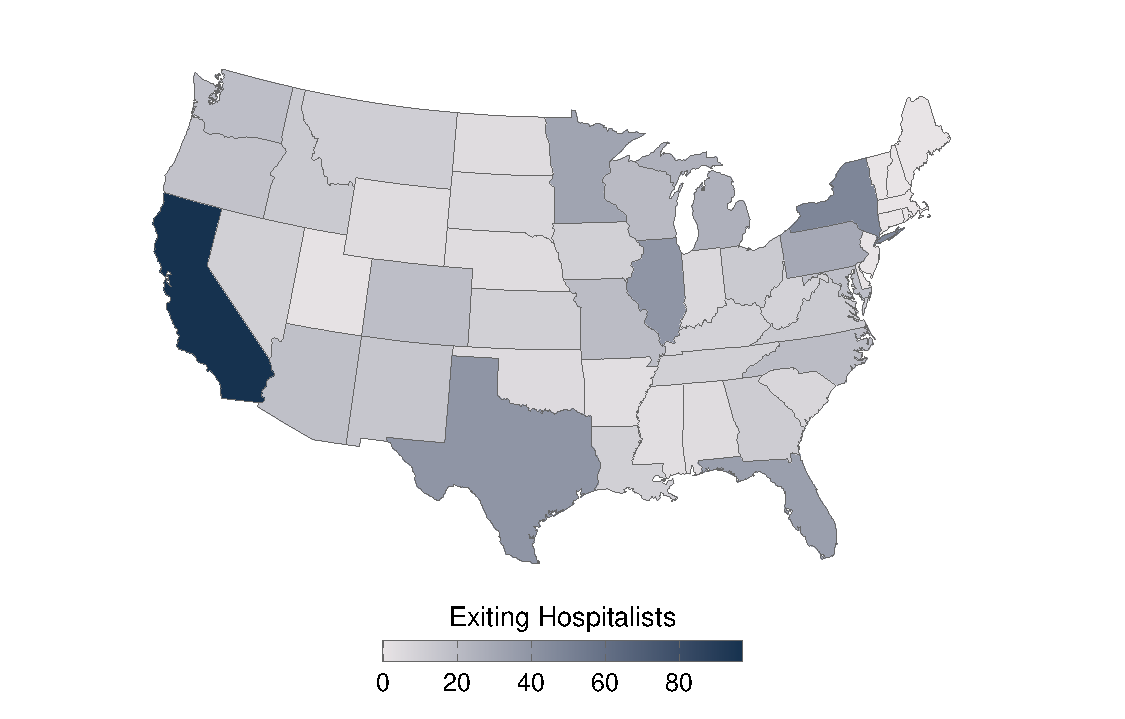
\includegraphics[width=.9\linewidth]{Objects/retire_map.pdf}
    \label{fig:retire_dist}
    \caption*{\footnotesize{\textit{Notes:} Map shows the number of hospitalists in the estimation sample who exit clinical practice at any point during the sample period, by state.}}
\end{figure}


The next set of outcomes measures the extent to which hospitalists shift work
into an office setting. MD-PPAS reports the share of a physician's claim line
items delivered in each place of service, and I use the office share directly as
a continuous outcome. I also construct an indicator equal to one if the physician
delivers any positive share of claims in an office, which captures movement on
the extensive margin. Where a physician appears in MD-PPAS but reports no claims
in a given place of service, I set the corresponding share to zero. For these outcomes I restrict the sample to physicians who never exit clinical
practice. Exit and a shift to office-based work are alternative responses to the
same underlying change, and including exiting physicians would conflate the two.
Because this restriction conditions on an outcome that treatment may itself
affect, the resulting sample is potentially selected; I report Lee (2009) bounds
in Section~\ref{sec:leebounds}.

As a proxy for what type of office physicians shift work towards, I construct a categorical measure of each hospitalist's billing entity type from the legal name of their primary tax affiliated organization (TIN) in MD-PPAS. I first collect the set of distinct names appearing in the sample, then apply a rule-based classifier that searches each name for category-specific keyword patterns, evaluated in the following priority order:
\begin{enumerate}
    \item \textbf{Staffing company}: names containing inpatient-staffing terminology (``hospitalist,'' ``hospital medicine,'' ``inpatient [consultant/physician/team/services/care]'') or matching known national or regional hospitalist, emergency medicine, or critical care staffing firms (e.g., TeamHealth, Sound Physicians, IPC Healthcare, EmCare, Schumacher, Apogee, Vituity, Cogent, 24 On Physicians, Emergency Staffing/Consults/Services Associates, Critical Care Consortium/Consultants).
    
    \item \textbf{Hospital-affiliated}: names containing ``hospital,'' ``medical center,'' ``health center,'' ``public hospital district,'' or ``hospitals corporation,'' indicating the physician bills directly under the hospital's own name; or names containing broader organizational terms consistent with a multi-specialty group, health system, or physician-organization structure affiliated with a hospital (e.g., ``health system,'' ``healthcare,'' ``medical foundation,'' ``medical group,'' ``physicians organization,'' ``clinic,'' ``permanente,'' ``physician network,'' ``primary care,'' ``medical associates,'' ``corporation,'' ``physician group,'' ``professional services,'' ``medical practice,'' and related variants).
    
    \item \textbf{Solo/independent}: names containing a physician title marker (``M.D.,'' ``DR.'') \textit{and} a small-practice legal suffix (``LLC,'' ``PLLC,'' ``PC,'' ``PA,'' ``SC,'' ``CHTD,'' ``LLP,'' or ``professional [medical] corporation''); or, separately, names matching small specialty-practice terminology (e.g., ``urgent care,'' ``family medicine/practice,'' ``gastroenterology,'' ``community care'') combined with a small-practice legal suffix.
\end{enumerate}

\noindent Some legal names, particularly small independent practices with idiosyncratic naming, do not match any keyword pattern above. For names left unclassified after the keyword-based step, I check whether the billing name contains the physician's own first and last name (exact substring match, case-insensitive) as recorded in MD-PPAS. If both the physician's first and last name appear in the TIN's legal name, I reclassify the entity as solo/independent, on the logic that a practice billing under the physician's own name is very likely that physician's individual or small private practice rather than an unrecognized organizational form. I apply this classification to the universe of distinct legal names appearing under either a physician's primary TIN, then merge the resulting category back onto the physician-year panel by legal name. 

Finally, I use the number of unique Medicare beneficiaries seen in a year as a measure of total patient volume in any setting, and the ratio of total claims to unique patients as a measure of billing intensity per patient. Both are reported directly in MD-PPAS. For these outcomes I impose two further restrictions. First, I keep only physicians who never exit. Second, I keep only physicians who remain hospital-based throughout the post-adoption period, defined as treating at least 70 percent of their patients in the inpatient setting in every year following EHR adoption. This holds the setting of practice fixed, so that movements in volume and billing intensity reflect changes in productivity within hospital-based practice rather than a reallocation of effort toward office-based work. As above, I account for selection on the included sample by employing Lee Bounds (\cite{lee2009training}). These volume measures reflect traditional fee-for-service Medicare only, so the estimated effects should be read as lower bounds on the change in a physician's total patient panel. 

For a subset of years I observe the composition of a physician's
billing activity for specific claims. The Medicare Physician and Other Practitioners public use file, which is
available from 2013 onward, reports the number of services delivered under each
 Healthcare Common Procedure Coding System (HCPCS) code. I group evaluation and management codes into eight categories:
initial hospital inpatient care, subsequent hospital inpatient care, hospital
discharge day management, hospital observation care, subsequent observation care,
critical care delivery, new patient office visits, and established patient office
visits. For each category I compute the share of a physician's total services
delivered under those codes. Because these data begin in 2013, and most
hospitalists in my sample are exposed to an electronic health record before then,
this analysis rests on a substantially smaller set of treated cohorts and I
present it as descriptive.


\subsection{Summary Statistics by Subgroup}

Table~\ref{tab:means_age} splits hospitalists at age 60. The two groups are
similar on most dimensions: they work with a comparable number of hospitals and hospital systems, and are affiliated with
hospitals at similar levels of physician-hospital integration. Older hospitalists
are exposed to an electronic health record roughly one year later on average
(2012 against 2011), a difference that reflects the hospitals they work with
rather than any individual choice.

\begin{table}[h]
\centering
\caption{Means by Age Group\label{tab:means_age}}
\centering
\begin{tabular}[t]{lcccccc}
\toprule
\multicolumn{1}{c}{ } & \multicolumn{2}{c}{Exit Sample} & \multicolumn{2}{c}{Office Sample} & \multicolumn{2}{c}{Productivity Sample} \\
\cmidrule(l{3pt}r{3pt}){2-3} \cmidrule(l{3pt}r{3pt}){4-5} \cmidrule(l{3pt}r{3pt}){6-7}
Variable & $<$60 & $\geq$60 & $<$60 & $\geq$60 & $<$60 & $\geq$60\\
\midrule
\addlinespace[0.3em]
\multicolumn{7}{l}{\textbf{Physician Characteristics}}\\
\hspace{1em}Number of Hospitals Worked With & 1.27 & 1.27 & 1.28 & 1.30 & 1.23 & 1.28\\
\hspace{1em}Female & 0.37 & 0.19 & 0.36 & 0.19 & 0.34 & 0.23\\
\hspace{1em}Number of Systems Worked With & 1.16 & 1.14 & 1.16 & 1.15 & 1.14 & 1.16\\
\hspace{1em}Age & 43.32 & 61.87 & 43.27 & 61.36 & 42.93 & 60.54\\
\addlinespace[0.3em]
\multicolumn{7}{l}{\textbf{EHR Exposure}}\\
\hspace{1em}Year of EHR Exposure & 2011 & 2012 & 2011 & 2012 & 2011 & 2012\\
\addlinespace[0.3em]
\multicolumn{7}{l}{\textbf{Outcome Variables}}\\
\hspace{1em}Ever Exit Clinical Work & 0.10 & 0.23 &  &  &  & \\
\hspace{1em}Fraction Claims in Office &  &  & 0.08 & 0.12 &  & \\
\hspace{1em}Work in an Office &  &  & 0.28 & 0.41 &  & \\
\hspace{1em}Number of Patients &  &  &  &  & 347 & 317\\
\hspace{1em}Claims per Patient &  &  &  &  & 3.41 & 4.02\\
\addlinespace[0.3em]
\multicolumn{7}{l}{\textbf{Employer Type}}\\
\hspace{1em}Hospital-Direct Employer &  &  & 0.50 & 0.53 &  & \\
\hspace{1em}Staffing Company Employer &  &  & 0.19 & 0.12 &  & \\
\hspace{1em}Solo/Independent Employer &  &  & 0.04 & 0.06 &  & \\
Num. Hospitalists & 4,419 & 1,052 & 3,988 & 810 & 1,958 & 279\\
\bottomrule
\end{tabular}
\begin{tablenotes}
\footnotesize
\item \textit{Note: } Summary statistics for the three main estimation samples split by whether a physician's maximum age observed in the sample is below or at/above 60. Age subgroups are fixed for each physician across all sample years based on their maximum observed age. Blank cells indicate a variable is not defined for, or not used in, that sample.
\end{tablenotes}
\end{table}


Two differences are substantial. First, older hospitalists are far less likely to
be female (19 percent, against 37 percent of those under 60) consistent with
the growth of women in medicine over the period during which these physicians
trained. Second, and more directly relevant to the analysis, older hospitalists
exit clinical practice at more than twice the rate: 23 percent against 10
percent. This difference motivates the age split and underlies the larger
absolute effect on exit reported for the older group. The office and productivity outcomes also differ at baseline. Older hospitalists
in the office sample see a larger share of patients in an office setting (12
percent against 8 percent) and are more likely to work in an office at all (41
percent against 28 percent). In the productivity sample they see somewhat fewer
Medicare patients (317 against 347) but bill more claims per patient (4.02
against 3.41). These baseline differences are important for interpreting the
heterogeneity results, since a given absolute effect represents a different
proportional change for each group.

\section{Heterogeneity by Hospital and Practice Characteristics}\label{sec:het}

The main analysis focuses on differential effects for hospitalists above and below 60 years of age. However, there are other factors that could potentially be correlated with how EHR exposure affects hospitalists. I therefore present average treatment effects for each outcome with the sample split between physicians in rural and urban areas, between those who typically work at small versus large hospitals, and between those affiliated with one hospital system versus more than one. Results are shown in Figure~\ref{fig:heter}. 

The effect of EHR adoption on physician exit is similar across all subgroups considered. The estimated increase in retirement is positive for physicians practicing in both small and large hospitals, in rural and urban settings, and among physicians affiliated with either one or multiple hospital systems. Although the point estimates vary somewhat, the confidence intervals overlap substantially and provide little indication that retirement responses differ systematically across practice environments. The increase in retirement therefore appears to reflect a broad response to EHR adoption rather than an effect concentrated among a particular type of hospitalist. The work-setting outcomes display somewhat more variation across groups, but the overall pattern remains consistent with the main analysis. EHR adoption increases both the share of claims submitted from office settings and the probability that a hospitalist performs any office-based work in every subgroup. The largest point estimates generally occur among hospitalists affiliated with more than one health system and among those practicing in rural areas, while somewhat smaller effects are observed for physicians in large hospitals. However, these differences are imprecisely estimated and the confidence intervals overlap considerably. As a result, the heterogeneity analysis provides little evidence that the shift toward office-based work is meaningfully stronger for any specific group of physicians. 

Finally, there is no clear evidence that productivity responses differ across subgroups. Point estimates for both the number of patients treated and claims per patient vary around the main estimate, but the confidence intervals are wide and include economically meaningful increases and decreases for several groups. Physicians affiliated with more than one health system again tend to exhibit somewhat larger positive estimates, particularly for patient volume, but these estimates are not statistically distinguishable from those observed elsewhere. Overall, the results suggest that the effects of EHR adoption are broadly similar across practice settings, with any apparent differences in magnitude largely attributable to sampling variation rather than systematic heterogeneity.


\begin{figure}[ht!]
\captionsetup{width=.9\linewidth}
    \centering
    \caption{Heterogeneity Analysis}
    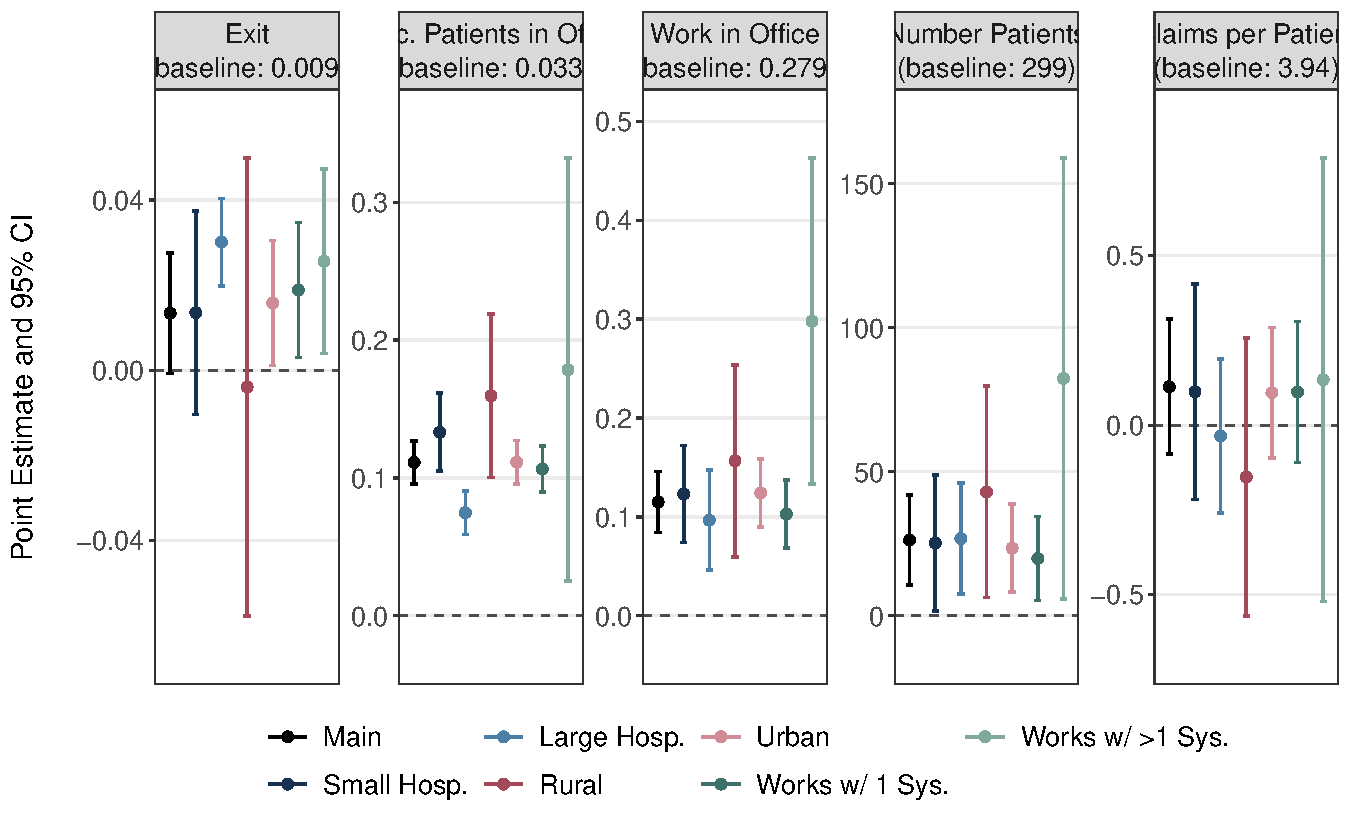
\includegraphics[width=\textwidth]{Objects/heterog_plot.pdf}
    \label{fig:heter}
    \caption*{\footnotesize{\textit{Notes:} Plot shows average group-time treatment effects for each outcome, estimated for the main specification (Main) and separately by subgroup: hospital size (Small Hosp., Large Hosp.), hospital location (Rural, Urban), and the number of distinct hospital systems the hospitalist works with (Works w/ 1 Sys., Works w/ $>$1 Sys.). Baseline pre-treatment means are reported in the panel subtitles. Confidence intervals are 95\% and calculated using the estimator of \citeauthor{callaway2021difference} (\citeyear{callaway2021difference}).}}
\end{figure}


\section{Potential Threats to Validity}\label{sec:alt}

\subsection{Other Hospital Changes}\label{sec:hospanalysis}

One potential concern is that EHR adoption coincides with other hospital
initiatives to improve productivity or quality, which would bias the results if the timing of EHR adoption is correlated with other changes. I address this by examining whether hospital behaviors change alongside EHR adoption. If such changes exist, they likely offset some EHR costs, suggesting that my estimates for exit and work setting are lower bounds on the true effects. However, this type of endogeneity would bias productivity results away from zero. 

I build a hospital-level data set covering 2009--2015 and examine observable hospital outcomes that might plausibly correlate with EHR adoption. I group these into three categories: non-EHR investments and organizational changes (capital expenditure on buildings and equipment, subsidiary ownership, administrator turnover, and bed counts); workforce changes (the number of nurses and physicians); and the extent of vertical integration with physicians (whether the hospital has an independent practice association, open or closed physician-hospital organization, or integrated salary model, together with the number of physicians at the hospital in each arrangement). 

Using the staggered difference-in-differences estimator of
\citet{callaway2021difference}, I
estimate the association between EHR adoption and each outcome. The results are shown in Table~\ref{tab:hosp_outcomes}. I do not interpret these estimates causally, but use them to assess whether other changes occur concurrently with adoption. Because the table reports fourteen outcomes, I adjust for multiple testing using the Benjamini-Hochberg procedure, which controls the false discovery rate. 

\begin{table}[!h][ht!]
\centering
\caption{\label{tab:hosp_outcomes}Association between EHR adoption and other hospital behaviors}
\centering
\begin{threeparttable}
\begin{tabular}[t]{>{\raggedright\arraybackslash}p{11em}cc>{\centering\arraybackslash}p{13em}cc}
\toprule
Outcome & Pre-treatment mean & Hospitals & Estimate [95\% CI] & BH $p$-value & Pre-trends\\
\midrule
\addlinespace[0.3em]
\multicolumn{6}{l}{\textbf{Non-EHR Investment/Organizational Changes}}\\
\hspace{1em}Capital Expenses: Buildings & 2,433,037 & 1,534 & 134,567 [-316,032, 585,167] & 0.80 & 0.78\\
\hspace{1em}Capital Expenses: Equipment & 1,668,741 & 1,532 & 218,919 [-9,222, 447,062] & 0.54 & 0.44\\
\hspace{1em}Owns Subsidiary & 0.156 & 1,516 & -0.000 [-0.025, 0.024] & 0.98 & 0.66\\
\hspace{1em}Change Admin & 0.155 & 1,540 & -0.011 [-0.053, 0.031] & 0.80 & 0.35\\
\hspace{1em}No. Beds & 109.6 & 1,540 & 4.064 [0.423, 7.705] & 0.52 & 0.11\\
\addlinespace[0.3em]
\multicolumn{6}{l}{\textbf{Workforce}}\\
\hspace{1em}No. Nurses & 124.0 & 1,540 & 4.168 [-1.526, 9.863] & 0.80 & 0.15\\
\hspace{1em}No. Physicians & 0.044 & 1,523 & -0.006 [-0.019, 0.008] & 0.80 & 0.52\\
\addlinespace[0.3em]
\multicolumn{6}{l}{\textbf{Physician Arrangements}}\\
\hspace{1em}Has IPA & 0.084 & 1,523 & 0.003 [-0.025, 0.030] & 0.90 & 0.34\\
\hspace{1em}Has OPHO & 0.761 & 1,523 & 0.015 [-0.012, 0.043] & 0.80 & 0.83\\
\hspace{1em}Has CPHO & 0.033 & 1,523 & 0.005 [-0.008, 0.018] & 0.80 & 0.07\\
\hspace{1em}Has FIO & 0.350 & 1,523 & -0.010 [-0.050, 0.030] & 0.80 & 0.41\\
\hspace{1em}No. Physicians, IPA & 12.9 & 1,523 & -4.032 [-13.4, 5.339] & 0.80 & 0.69\\
\hspace{1em}No. Physicians, CPHO & 6.915 & 1,523 & -0.796 [-5.477, 3.886] & 0.89 & 0.26\\
\hspace{1em}No. Physicians, FIO & 12.8 & 1,520 & 3.755 [-3.341, 10.9] & 0.80 & 0.53\\
\bottomrule
\end{tabular}
\begin{tablenotes}
\item \textit{Note: } 
\item Each row reports the overall average treatment effect on the treated from Callaway and Sant'Anna (2021), aggregated over event time, with the 95% confidence interval in brackets. $p$-values are adjusted across all outcomes in the table using the Benjamini--Hochberg procedure to control the false discovery rate. The pre-trends column reports a Wald test of the null that all pre-treatment group-time effects equal zero. $^{*}p<0.10$, $^{**}p<0.05$, $^{***}p<0.01$.
\end{tablenotes}
\end{threeparttable}
\end{table}


Panel A considers non-EHR investments and organizational changes. EHR adoption is not associated with statistically significant changes in capital expenditures on buildings or equipment, hospital ownership of subsidiaries, or administrative turnover. The point estimates are economically modest relative to pre-treatment means and are estimated imprecisely. Although the coefficient on the number of beds is positive, the estimate is small relative to the average hospital size and does not survive adjustment for multiple hypothesis testing. More generally, the absence of effects on these outcomes suggests that EHR adoption is not occurring alongside broader organizational restructuring or major investments unrelated to information technology.

The second set of outcomes examines hospital workforce composition. I find no evidence that adopting hospitals systematically expand or contract their clinical workforce following EHR implementation. The estimated effect on the number of nurses is positive but imprecisely estimated, while the effect on the number of physicians is economically small and statistically indistinguishable from zero. These results alleviate concerns that the main findings could be driven by contemporaneous changes in staffing levels rather than by EHR adoption itself.

Finally, I consider physician organizational arrangements, including participation in independent practice associations (IPAs), open physician-hospital organizations (OPHOs), closed physician-hospital organizations (CPHOs), and fully integrated organizations (FIOs). EHR adoption has no detectable effect on the likelihood that a hospital maintains any of these arrangements. Similarly, I find no evidence of changes in the number of affiliated physicians within any organizational form. While several coefficients are positive and others negative, none are statistically distinguishable from zero, and the estimates lack a consistent pattern across outcomes.

Taken together, these results provide little evidence that EHR adoption is correlated with changes in other observable hospital behaviors. The absence of systematic effects across investment, organizational, workforce, and physician-affiliation measures supports the interpretation that the main estimates are not capturing broader changes in hospital operations that coincide with EHR adoption. While I cannot rule out unobserved changes, the absence of observable ones mitigates the concern that concurrent hospital initiatives drive the main findings.

\subsection{Changes Related to Medicare Patients}\label{sec:aca}

Many changes under the Affordable Care Act (ACA) from 2010--2014, such as
insurance expansion and hospital quality initiatives, affected healthcare
delivery. For these changes to bias my results, they would need either to drive hospital EHR adoption or to affect hospitalists exposed to EHRs differently from those not yet exposed. Three concerns are worth addressing relating to this. 

First, if the results were driven by hospitals adopting EHRs in 2012, when pay-for-performance initiatives took effect, or in 2014, when Medicaid expansion began, then ACA policies rather than EHR exposure could account for the observed changes in physician behavior. I present average group-time treatment effects separately by adoption cohort in Appendix~\ref{sec:changes}. The estimates are similar across cohorts with no
strong discontinuity for the 2012 or 2014 cohorts. For an ACA policy to generate this pattern, it would have to have affected treated and comparison hospitalists differentially in every adoption year rather than at the specific dates when major provisions took effect. Second, the ACA had potentially opposing effects on the Medicare population:
increased demand for Medicaid could crowd out Medicare patients, while changes to Medicare itself might increase utilization.
\citet{carey2020impact} find no evidence of spillovers from Medicaid expansion
onto Medicare utilization, which limits the scope for either channel to explain the results. Third, hospitalists might exit Medicare practice in order to treat privately insured patients instead. This is unlikely for three reasons: EHR adoption is not plausibly correlated with the insurance composition of a hospital's patients, hospitalists typically cannot select patients on the basis of insurance, and no hospitalist in my sample opted out of Medicare according to CMS records.

Therefore, concurrent changes affecting
Medicare patients are unlikely to account for whole of the results shown. The identifying variation comes from the timing of EHR adoption across hospitals, and the consistency of the estimates across adoption cohorts is difficult to reconcile with an explanation resting on policies that took effect at particular dates.

\subsection{Change in Claim Coding}\label{app:coding}

Another potential concern is that observed changes in place of work claims are not due to physical relocation, but instead are due to a change in how claims are coded. If EHRs digitize coding practices, they could be correlated with such a procedure. In this section, I investigate which specific services drive the increase in office-based work documented in Section~\ref{sec:office}. I merge the CMS Medicare Physician \& Other Practitioners public use file, which reports claims by provider, HCPCS code, and place of service beginning in 2013. Because this file is not available before 2013, I restrict this analysis to 2013--2017. I group evaluation and management codes into eight categories, covering hospital-based care (initial and subsequent inpatient care, discharge management, and observation care, both initial and subsequent), critical care delivery, and office-based care (new and established patient visits), and compute each physician's share of total claims in each category. I then estimate the effect of EHR exposure on these shares using the same specification as the main results, with the not-yet-treated hospitalists in this restricted panel serving as the comparison group. Because the panel begins after most hospitalists in the main sample are already exposed, the comparison group here is smaller and less balanced across cohorts than in the main analysis; I therefore report these estimates as descriptive rather than causal.

Figure \ref{fig:claims_estimates} reports the results in two panels. The left panel includes all hospitalists except those who exit; the right panel further restricts to those who remain primarily hospital-based throughout, the same restriction used for the patient volume outcomes in Section~\ref{sec:patientcount}. In the full sample, established patient office visits are the only category with a statistically significant change, rising by roughly 2 percentage points. Every hospital-based category is indistinguishable from zero. In the restricted panel, the established-patient effect also disappears, consistent with it being driven by hospitalists who take on office-based work rather than by any change in how hospital-based hospitalists bill their inpatient encounters. This pattern indicates that the increase in office-based practice does not operate through a reallocation of billing codes among hospitalists who continue working primarily in the hospital. New and established patient office visits (HCPCS codes 99202--99215) can only be billed in an office setting, whereas the hospital-based categories that remain unchanged, such as subsequent inpatient care (99231--99233), describe evaluation and management of a patient already admitted. The absence of any change in the hospital-based categories, in either panel, suggests that hospitalists are not billing their inpatient encounters differently; rather, the physicians driving the office result are those who have begun seeing patients in an office setting at all, consistent with the extensive-margin finding in Section~\ref{sec:office}.

\begin{figure}[ht!]
\captionsetup{width=.9\linewidth}
    \centering
    \caption{Effect of EHR Exposure on Type of Claims}
    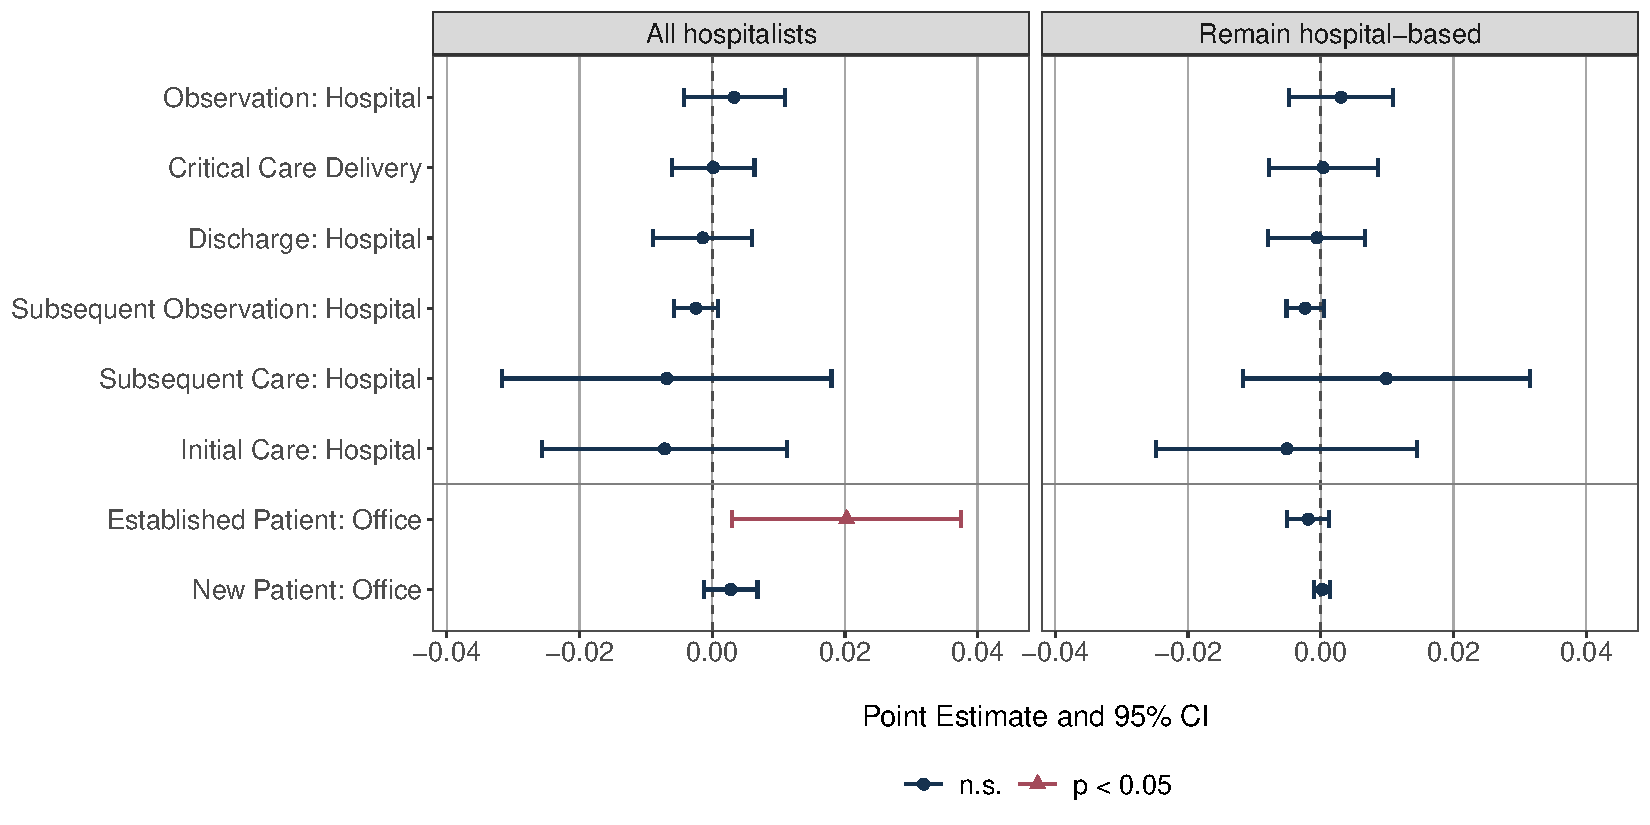
\includegraphics[width=\textwidth]{Objects/claim_type_results.pdf}
    \label{fig:claims_estimates}
    \caption*{\footnotesize{\textit{Notes:} Plot shows average group-time treatment effects on each physician's share of total claims in a given billing-code category, estimated using the CMS Medicare Physician \& Other Practitioners public use file, 2013--2017. The left panel includes all hospitalists except those who retire; the right panel further restricts to hospitalists who remain primarily hospital-based throughout the sample, the same restriction used for the patient volume outcomes. Confidence intervals are 95\%.}}
\end{figure}





\subsection{Ambulatory EHRs}\label{sec:ambulatory_timing}

A concern with interpreting the shift toward exit or office-based work documented in
Sections ~\ref{sec:retire} \& ~\ref{sec:office} as caused by inpatient EHR exposure is that the HITECH
Act incentivized the adoption of electronic health records in both hospital and
ambulatory settings simultaneously. If ambulatory EHR adoption occurred at the
same time as the hospital adoption I use for
identification, then hospitalists who appear to relocate toward office-based
work in response to inpatient EHR burden may in fact have been moving toward a
setting that was, or was about to be, similarly burdensome. This section
addresses this concern along three dimensions: the relative timing of inpatient
and ambulatory adoption, the relative functional complexity of inpatient and
ambulatory systems, and the direction in which any remaining correlation in
adoption timing would bias the estimates. I compare the timing of inpatient and ambulatory EHR adoption using two
independent data sources. 

The first is the HIMSS Analytics, which surveys hospitals
and hospital-owned ambulatory entities on whether specific clinical applications
are live and operational. Unlike the hospital-side data, HIMSS does not record
ambulatory adoption at the level of individual clinical functions: it tracks
ambulatory systems as a single undifferentiated ``Ambulatory'' category
containing three items: Ambulatory EMR, Practice Management, and Ambulatory
PACS, of which only Ambulatory EMR constitutes clinical documentation
functionality comparable to what I measure on the hospital side. This lack of
granularity means the physician-facing measure I use in the main analysis, which
requires computerized physician order entry, physician documentation, or a
physician portal specifically, has no direct ambulatory counterpart. I therefore
construct the timing comparison in this section using the broadest available
hospital-side measure: whether any of the six tracked clinical components,
including but not limited to the physician-facing ones, is live and
operational. Because hospital adoption of
physician-facing components typically follows adoption of at least one other
clinical component, this broader hospital-side measure adopts weakly earlier
than my main physician-facing measure, so any timing gap identified here is, if
anything, an understatement of the true gap between the technology hospitalists
in my sample are exposed to and the technology available in the ambulatory
settings they might move toward. Figure~\ref{fig:timing_evidence} reports the
share of each setting with EMR live and operational, by year. In 2009, 92.5 percent of surveyed hospitals already had EMR live,
compared with 42.4 percent of surveyed ambulatory entities, a gap of 50.1
percentage points. This gap narrowed steadily over the sample period but did not
close: by 2015, the final year of the panel, 98.4 percent of hospitals had EMR
live compared with 87.3 percent of ambulatory entities, a gap of 11.1 percentage
points.


The second source is Meaningful Use attestation data from the Office of the
National Coordinator for Health Information Technology (ONC), which records the
Meaningful Use stage each provider attested to under the Medicare and Medicaid
EHR Incentive Programs. Stage 2, which introduced more demanding interoperability
and patient-engagement requirements, first took effect in 2014. In that year,
40.6 percent of attestations using an inpatient-certified product had progressed
to Stage 2, compared with 25.6 percent of attestations using an
ambulatory-certified product. As with the HIMSS comparison, this gap narrowed
over time, falling to 0.7 percentage points in 2015 and 1.6 points in 2016. Both
data sources therefore indicate that inpatient EHR adoption led ambulatory
adoption throughout the sample period, and particularly during its early years,
when most of the hospital adoption events I use for identification occur.

%\begin{table}[!h]
\centering
\caption{\label{tab:himss_timing}Share of HIMSS-surveyed entities with EMR live and operational, by setting}
\centering
\begin{threeparttable}
\begin{tabular}[t]{cccc}
\toprule
Year & Hospital (\%) & Ambulatory (\%) & Gap (p.p.)\\
\midrule
2009 & 92.5 & 42.4 & 50.1\\
2010 & 93.4 & 44.9 & 48.5\\
2011 & 94.2 & 51.3 & 42.8\\
2012 & 94.3 & 61.9 & 32.4\\
2013 & 95.6 & 75.8 & 19.8\\
\addlinespace
2014 & 97.1 & 83.5 & 13.6\\
2015 & 98.4 & 87.3 & 11.1\\
\bottomrule
\end{tabular}
\begin{tablenotes}
\item \textit{Note: } 
\item Hospital share is based on any of six clinical EMR sub-components (clinical data repository, clinical decision support, computerized physician order entry, order entry, patient portal, or physician documentation) reported live and operational. Ambulatory share is based on the Ambulatory EMR application, the only comparable clinical documentation system HIMSS tracks for this setting.
\end{tablenotes}
\end{threeparttable}
\end{table}


\begin{figure}[ht!]
    \centering
    \captionsetup{width=.7\linewidth}
    \caption{Timing of EHR Adoption in Ambulatory versus Inpatient Setting}
    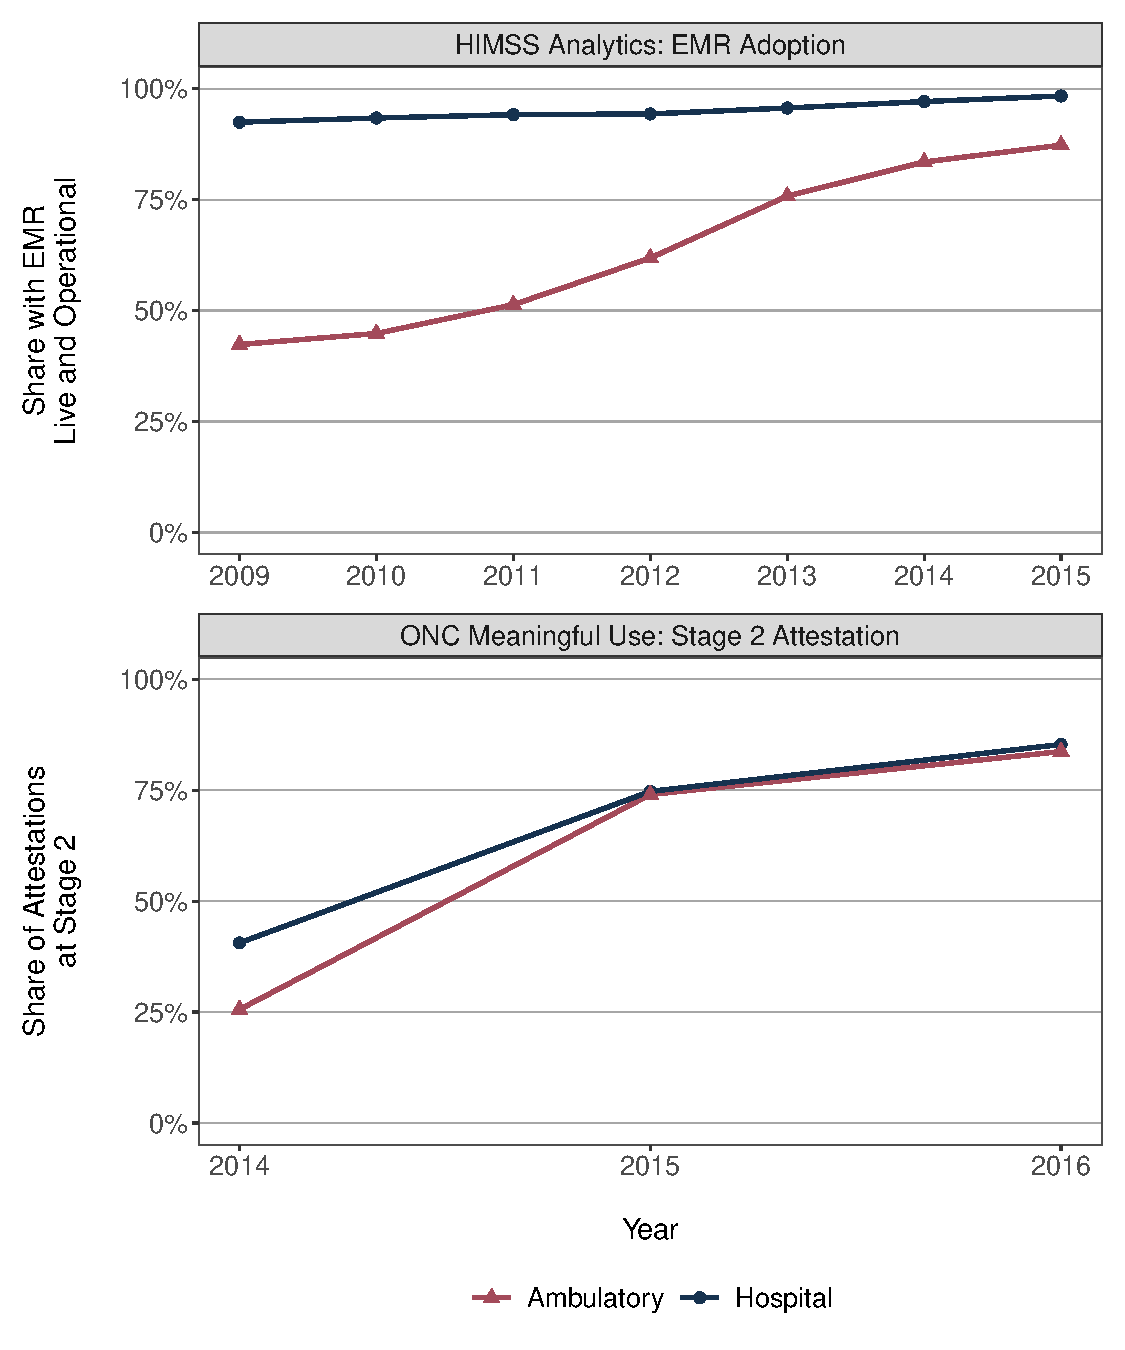
\includegraphics[width=0.7\textwidth]{Objects/timing_evidence_panels.pdf}
    \label{fig:timing_evidence}
    \caption*{\footnotesize{\textit{Notes:} Top panel shows the share of surveyed hospital and hospital-owned ambulatory entities with any of six tracked electronic medical record (EMR) components live and operational, by year, using HIMSS Analytics data. Bottom panel shows the share of Meaningful Use attestations under the Medicare and Medicaid EHR Incentive Programs that had progressed to Stage 2, by inpatient- versus ambulatory-certified product, using data from the Office of the National Coordinator for Health Information Technology (ONC).}}
\end{figure}

 
A limitation of this comparison is the HIMSS ambulatory sample is
restricted to hospital-owned outpatient clinics, since HIMSS does not survey
independent ambulatory practices. Hospital-owned clinics plausibly have access
to their parent hospital's information technology budget, staff, and vendor
relationships, and are therefore likely to adopt more quickly than an average
independent practice would. If even this comparatively well-resourced segment of
the ambulatory market lagged hospital adoption, the true gap between hospital and independent
ambulatory adoption is plausibly larger, not smaller. 
 
A second dimension of the concern is that even if ambulatory EHR adoption lagged
inpatient adoption, a hospitalist moving to an office setting might still
encounter an EHR shortly after, undermining a full escape from
technology-related burden. The HIMSS taxonomy provides indirect evidence that
this concern is of limited quantitative importance, because ambulatory systems
are recorded as functionally simpler than inpatient systems even where adopted. HIMSS tracks hospital electronic medical record adoption across six distinct clinical components, described above. Ambulatory adoption, by contrast, is
tracked as three items under a single "Ambulatory" category---Ambulatory EMR,
Practice Management, and Ambulatory PACS---of which only Ambulatory EMR
constitutes comparable clinical documentation functionality; the other two are
operational and imaging systems rather than systems a physician uses to document
patient care. This asymmetry in HIMSS's own data collection is suggestive of a
broader industry understanding that ambulatory systems during this period
offered a narrower range of clinical functionality than inpatient systems.
 
Consistent with this, among hospitals with any live clinical EMR component, the
median hospital has 5 of the 6 tracked components live and operational (mean
4.85, across 35,890 hospital entity-years). No comparable multi-component measure
is available for ambulatory entities, since only one clinical component is
tracked for that setting. A hospitalist who relocates to an office setting before
or shortly after that setting's Ambulatory EMR system goes live is therefore
likely to face a narrower set of required clinical documentation tasks than the
hospitalist faced in the inpatient setting, even setting aside the timing gap
documented above.
  
Even granting some correlation between inpatient and ambulatory adoption timing,
the direction in which this would bias my estimates  plausibly works against finding a positive effect on office-based work. As discussed in Section ~\ref{sec:background}, a
hospitalist's decision to shift labor market behavior reflects the expected utility of
working in each setting, which a forward-looking physician would form using not
only the current EHR burden in each setting but also their expectations about
future EHR burden. If hospitalists correctly anticipated that ambulatory EHR
adoption was coming soon nationally, this anticipation would be incorporated into the expected
utility of relocating, narrowing rather than widening the utility gap between
remaining in the hospital and moving to an office setting. Under this interpretation, the positive effect I estimate on office-based work is a lower bound: hospitalists appear to shift toward office-based practice even though
that setting's technological advantage was not expected to persist indefinitely.
A hospitalist responding only to current, realized burden differentials, with no
forward-looking adjustment, would face no such attenuation. In neither case does
correlated ambulatory adoption bias the estimated office-based effect away from zero in a
direction that would overstate the paper's central finding.

The same reasoning does not necessarily apply to exit from clinical practice. A hospitalist who would otherwise move to an office setting to avoid inpatient EHR use, but who expects ambulatory adoption to follow soon, may instead choose to leave clinical practice altogether. To the extent that expected ambulatory adoption is correlated with hospital adoption timing, part of the estimated exit effect may therefore reflect anticipated EHR exposure in ambulatory settings rather than inpatient adoption alone. I therefore interpret the exit estimate as the effect of hospital EHR exposure in an environment where EHR-free alternatives were expected to diminish, rather than as the effect of inpatient adoption in isolation. This interpretation is consistent with the concentration of exit effects among hospitalists aged 60 and over, for whom relocating to a setting expected to adopt EHRs soon is comparatively less attractive than retiring.


\section{Sensitivity Analysis}\label{app:sensitive}


\subsection{Honest Difference-in-differences}

Table~\ref{tab:honest_breakdown} collects the sensitivity analysis discussed alongside each outcome above. Following \citet{rambachan2019honest}, I bound each treatment effect under the restriction that any post-treatment violation of parallel trends is at most $\bar{M}$ times the largest violation observed before treatment, and report the breakdown value at which the robust confidence interval first includes zero. The results suggest substantial variation in the sensitivity of the estimates to departures from parallel trends. Both office-work outcomes are highly robust: the estimated effects remain statistically significant for values of $\bar{M}$ greater than two, implying that the conclusions would survive post-treatment violations more than twice as large as any deviation observed in the pre-period. In contrast, the remaining outcomes are considerably more sensitive. The breakdown values for exit, patient volume, and claims per patient are all 0.25, indicating that relatively modest departures from parallel trends would be sufficient to render these estimates statistically indistinguishable from zero. Overall, the office-work findings appear substantially more robust to potential trend violations than the exit and productivity results.

\begin{table}[!h]
\centering
\caption{\label{tab:honest_breakdown}Robustness to violations of parallel trends}
\centering
\begin{threeparttable}
\begin{tabular}[t]{lccc}
\toprule
Outcome & Original 95\% CI & Largest pre-treatment violation & Breakdown $\bar{M}$\\
\midrule
Exit & {}[0.0036, 0.0300] & 0.0035 & 0.25\\
Fraction in Office & {}[0.0976, 0.1277] & 0.0044 & $>2$\\
Work in Office & {}[0.0935, 0.1535] & 0.0053 & $>2$\\
Number Patients & {}[4.69, 34.81] & 5.76 & 0.25\\
Claims per Patient & {}[-0.4105, -0.0636] & 0.1937 & 0.25\\
\bottomrule
\end{tabular}
\begin{tablenotes}
\item \textit{Note: } 
\item Sensitivity analysis follows Rambachan and Roth (2023). The restriction bounds any post-treatment violation of parallel trends at $\bar{M}$ times the largest violation observed before treatment. The breakdown value is the smallest $\bar{M}$ at which the robust confidence interval includes zero; values are searched on a grid of width 0.05 up to $\bar{M}=2$. The event window is restricted to $e \in [-3, 4]$.
\end{tablenotes}
\end{threeparttable}
\end{table}


\subsection{Lee Bounds for Sample Selection}\label{sec:leebounds}

EHR exposure affects which hospitalists are included in the analysis for both office work outcomes and patient count outcomes (since I drop those who exit or move), indicating a non-random attrition problem. That is, if productive hospitalists are the ones who do not change their behavior after EHR exposure, the estimates are biased. To investigate whether my results are robust to this issue, I construct average treatment effect bounds as in  \citeauthor{lee2009training} (\citeyear{lee2009training}). If the hospitalists who left would have had systematically high or low outcomes had they remained, their absence shifts the estimate. To bound this, I trim 3.3 percent from the treated group's outcome distribution. Trimming from the bottom assumes the hospitalists who left would have had the lowest outcomes and gives the upper bound; trimming from the top assumes the opposite and gives the lower bound. For these bounds to be valid, a monotonicity assumption must hold on selection. In this case, EHR exposure must increase the likelihood of exiting or moving workplace settings and no hospitalists remain in the sample under treatment who would have exited or moved in the absence of EHR exposure. Since I find in earlier analyses that hospitalists are more likely to move and exit due to EHRs, this assumption is reasonable. I present the lower and upper bounds in Table \ref{leebouns}, and they confirm that even if there is non-random sample selection, the qualitative results still hold. 

\import{Table Code}{leebounds.tex}

\subsection{Never-Treated Comparison Groups}
\label{sec:nevertreated}

My main specification drops hospitalists not exposed to an EHR by 2015, so that identification comes from comparisons with not-yet-treated physicians. An alternative is to truncate the panel at 2015 and retain those never exposed
within that window as a comparison group. This section reports that specification and explains why I do not adopt it.

Table~\ref{tab:nt_chars} compares the two groups in 2009, the first year of the panel. Never-treated hospitalists differ from treated hospitalists on nearly every observable dimension. They are older by 3.4 years on average and have been in practice two years longer. They work at substantially smaller hospitals: 165 beds on average, against 268 for the treated, and with fewer hospitals and fewer distinct hospital systems. Most consequentially for the outcomes I study, they are already less hospital-based at baseline: 76.8 percent of their claims are inpatient, against 83.4 percent for the treated, and 12.0 percent are delivered in an office setting, against 7.1 percent. All of these differences are statistically significant at conventional levels. These differences are not incidental to the setting. Meaningful Use incentives were substantial over this period, and hospitals that had still not adopted an
EHR by 2015 were disproportionately small. Hospitalists affiliated with them are correspondingly a selected group, and one that is already further along the transition toward office-based practice that I study.

\begin{table}[!h]
\centering
\caption{\label{tab:nt_chars}Characteristics of treated and never-treated hospitalists}
\centering
\begin{threeparttable}
\begin{tabular}[t]{lcccc}
\toprule
Variable & Treated & Never treated & Difference & $p$-value\\
\midrule
Average hospital beds & 268 & 165 & -102 & $<$0.01\\
Years since graduation & 14.45 & 16.46 & 2.01 & $<$0.01\\
Female & 0.335 & 0.342 & 0.007 & 0.73\\
Age & 50.88 & 54.24 & 3.35 & $<$0.01\\
Medicare patients & 278 & 257 & -21.30 & 0.04\\
\addlinespace
Hospitals worked with & 1.21 & 1.09 & -0.120 & $<$0.01\\
Systems worked with & 1.10 & 1.05 & -0.052 & $<$0.01\\
Share of claims, inpatient & 0.834 & 0.768 & -0.066 & $<$0.01\\
Share of claims, office & 0.071 & 0.120 & 0.049 & $<$0.01\\
\bottomrule
\end{tabular}
\begin{tablenotes}
\item \textit{Note: } 
\item Means measured in 2009, the first year of the panel. Never-treated hospitalists are those with no EHR-adopting hospital affiliation through 2015. $p$-values are from two-sided $t$-tests of equality of means.
\end{tablenotes}
\end{threeparttable}
\end{table}


Table~\ref{tab:nt_estimates} shows what this implies for the estimates. Both columns use the same panel truncated at 2015, so the only difference between them is the comparison group. The estimated effect on exit from clinical practice changes sign entirely, from 0.013 under not-yet-treated comparisons to $-0.127$ under never-treated comparisons. The latter estimate implies that EHR exposure reduces the probability of leaving practice by nearly 13 percentage points, an implausible magnitude against a counterfactual cumulative exit rate of roughly 8 percent. The explanation is visible in Table~\ref{tab:nt_chars}: never-treated hospitalists are more than three years older and closer to retirement, so they accumulate exits faster for reasons unrelated to EHR adoption, which makes exposure appear protective.

The office outcomes move in a similar direction for a similar reason. The
estimated effect on the fraction of patients seen in an office falls from 0.111 to 0.047, and on the indicator for working in an office from 0.115 to 0.067. Because never-treated hospitalists already see a substantially larger share of patients in an office at baseline, the two groups are at different points in the same transition, and differencing between them attributes to EHR exposure only the part of the shift that exceeds what the comparison group was already doing. The effect on patient volume is larger under never-treated comparisons (35.2 versus 18.5 patients). I therefore rely on not-yet-treated comparisons as the main specification. 

\begin{table}[ht!]
\centering
\caption{\label{tab:nt_estimates}Estimates using not-yet-treated and never-treated comparison groups}
\centering
\begin{threeparttable}
\begin{tabular}[t]{lcccc}
\toprule
\multicolumn{1}{c}{ } & \multicolumn{4}{c}{Comparison group} \\
\cmidrule(l{3pt}r{3pt}){2-5}
Outcome & Not-yet-treated & N (NYT) & Never-treated & N (NT)\\
\midrule
Exit from Clinical Practice & 0.013 (0.008) & 5,471 & -0.127 (0.012) & 6,023\\
Fraction of Claims in Office & 0.111 (0.008) & 4,798 & 0.047 (0.013) & 5,166\\
Works in an Office & 0.115 (0.017) & 4,798 & 0.067 (0.018) & 5,166\\
Number of Patients & 18.52 (7.43) & 2,237 & 35.24 (11.30) & 2,359\\
\bottomrule
\end{tabular}
\begin{tablenotes}
\item \textit{Note: } 
\item Both columns use a panel truncated at 2015. The not-yet-treated column excludes hospitalists never exposed within that window; the never-treated column retains them and uses them as the comparison group. Standard errors in parentheses, clustered at the physician level.
\end{tablenotes}
\end{threeparttable}
\end{table}


\subsection{Alternative Estimators}\label{app:estimators}

A robust recent literature documents that two-way fixed effects estimators can be badly biased under staggered treatment timing with heterogeneous treatment effects, since the implied comparisons can place negative weight on some treated units \citep[e.g.,][]{goodman2021difference, sun2021estimating}. To avoid these problems, I use the group-time average treatment effect estimator of \citet{callaway2021difference} as my main specification. In this section I compare it against three alternatives: two-way fixed effects, the two-stage estimator of \citet{gardner2021two}, and the stacked regression approach used by \citet{cengiz2019effect}.
I first estimate a standard two-way fixed effects event study,

$$\text{outcome}_{i,t} = \sum_{j=-4}^{-2} \beta_j  \text{ rel-year}_{j} + \sum_{j=0}^{4} \beta_j \text{ rel-year}_{j} + \delta_i + \gamma_t + \varepsilon_{i,t},$$

\noindent where $\text{rel-year}_j$ is an indicator for being $j$ years from first EHR exposure, $\delta_i$ are physician fixed effects, and $y_t$ are year fixed effects. 

The two-stage estimator of \citet{gardner2021two} addresses negative weighting issues by first partialling out unit and time fixed effects using only untreated observations, then estimating treatment effects in a second stage. I implement it with the same not-yet-treated comparison group and sample restrictions used in the main specification, so that any difference from the \citet{callaway2021difference} estimates reflects the estimator rather than the sample. The stacked regression approach of \citet{cengiz2019effect} re-frames the staggered design as a set of separate sub-experiments, one for each treatment cohort, each stacked with its own set of clean controls and its own unit and time fixed effects. I define each cohort's sub-experiment over a window from one year before to four years after treatment, matching the post-treatment horizon used elsewhere in the paper, and average the post-treatment coefficients within each stack before combining across cohorts. As with two-stage difference-in-differences, I apply the same sample restrictions as the main specification within each stack.

Figure \ref{fig:estimators} reports the overall average treatment effect from all approaches including the main specification, in the same units as the outcome, alongside the pre-treatment mean for reference. For physician exit, the two-stage and stacked estimates are close to the main specification, while the two-way fixed effects estimate is smaller and statistically indistinguishable from zero. Despite these differences in magnitude, all four estimators imply a positive effect of EHR adoption on exit. The office-work outcomes show the largest differences across estimators. For both the fraction of claims submitted in office settings and the probability of performing any office-based work, the two-stage and stacked estimators produce estimates similar to the main specification. In contrast, the two-way fixed effects estimates are close to zero and, in the case of the work-in-office outcome, slightly negative. This pattern is consistent with the negative-weighting concerns that motivate the use of alternative estimators in settings with staggered treatment adoption. 

\begin{figure}[ht!]
\captionsetup{width=.9\linewidth}
    \centering
    \caption{Alternative Estimators}
    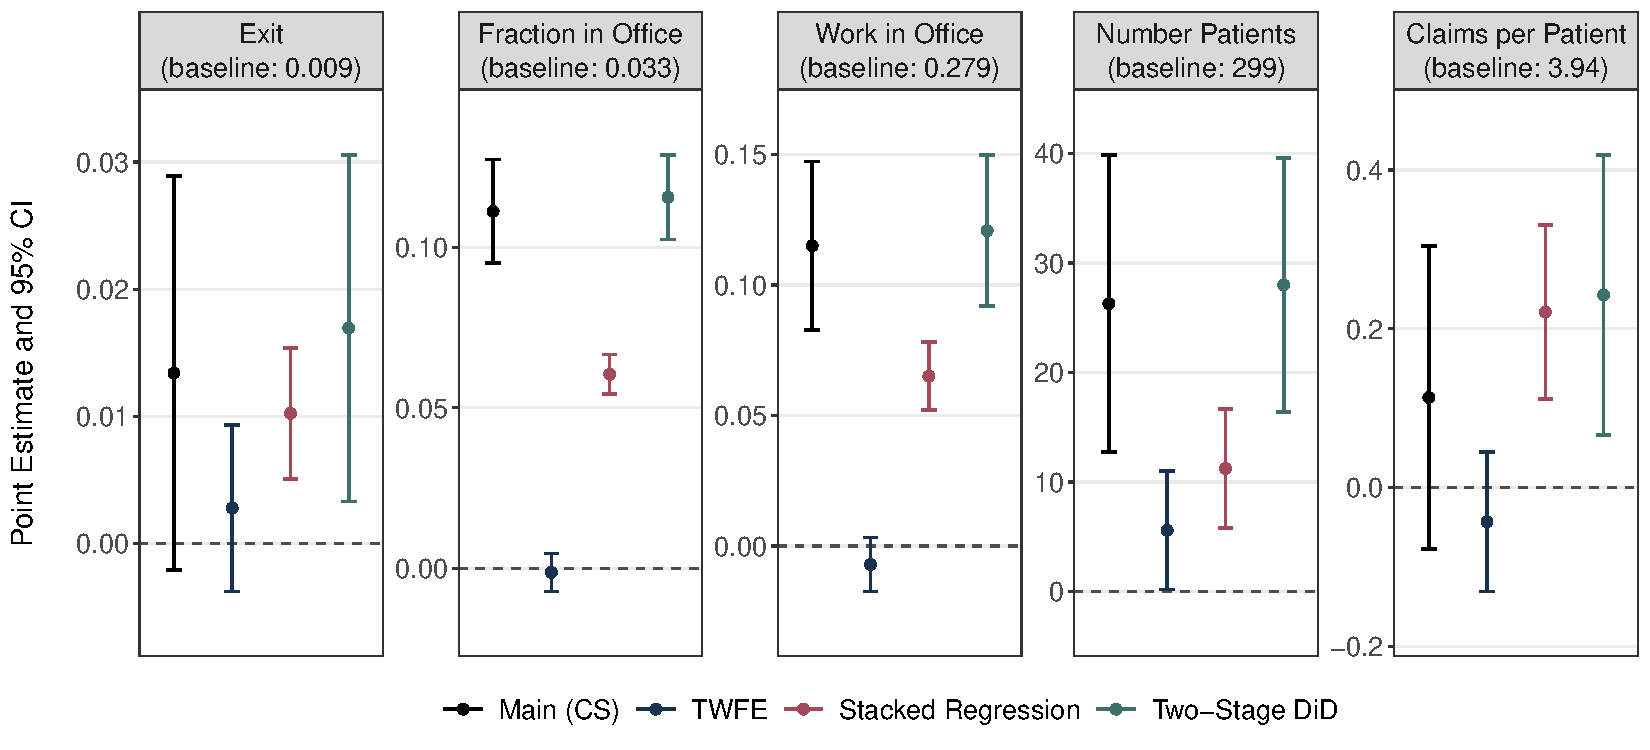
\includegraphics[width=\textwidth]{Objects/estimators_plot.pdf}
    \label{fig:estimators}
    \caption*{\footnotesize{\textit{Notes:} Plot shows the overall average treatment effect on the treated for each outcome under four estimators: the group-time average treatment effect estimator of \citeauthor{callaway2021difference} (\citeyear{callaway2021difference}), used as the main specification (Main (CS)); a standard two-way fixed effects event study (TWFE); the stacked regression approach of \citeauthor{cengiz2019effect} (\citeyear{cengiz2019effect}); and the two-stage estimator of \citeauthor{gardner2021two} (\citeyear{gardner2021two}). Baseline pre-treatment means are reported in the panel subtitles. Confidence intervals are 95\%.}}
\end{figure}

The remaining outcomes are broadly similar across estimators. For patient volume, all four approaches produce positive point estimates, although there is noticeable variation in magnitude and precision. Likewise, all estimators indicate a decline in claims per patient following EHR adoption, though the estimated effect ranges from modest under the stacked specification to substantially larger under the two-stage estimator. The wider confidence intervals for these productivity measures likely reflect the smaller samples available for these outcomes. Overall, the alternative estimators produce conclusions that closely mirror those from the main specification: EHR adoption increases exit and office-based work, while the estimated productivity effects are positive but less precisely determined.


\subsection{Robustness to a Balanced Cohort Sample}\label{sec:balanced}

Because EHR exposure is staggered across cohorts, different event-study coefficients are identified using different, and potentially non-overlapping, sets of treatment cohorts. To assess whether my main results are sensitive to this composition, I re-estimate each outcome using only hospitalists first exposed to EHRs in 2012--2014, the cohorts for which a full, symmetric event-time window of three years before and three years after exposure is observed. Table \ref{tab:balanced_robustness} compares the overall average treatment effect on the treated from this balanced-cohort sample to the corresponding estimate from the main specification, which pools all cohorts.

\begin{table}[!h]
\centering
\caption{\label{tab:balanced_robustness}Robustness to Balanced Cohort Sample (Cohorts 2012--2014, Event Window $-3$ to $+3$)}
\begin{threeparttable}
\begin{tabular}[t]{lllll}
\toprule
Outcome & Main Sample & Balanced Sample & Pre-Trends $p$ & N Physicians\\
\midrule
Ever Exit Clinical Work & 0.013 (0.007) & 0.006 (0.007) & 0.57 & 2,133\\
Fraction Claims in Office & 0.111 (0.008) & 0.073 (0.006) & 0.18 & 1,866\\
Work in an Office & 0.115 (0.016) & 0.077 (0.015) & 0.24 & 1,866\\
Number of Patients & 18.521 (7.6) & 13.146 (6.439) & 0.96 & 860\\
Claims per Patient & -0.246 (0.096) & -0.178 (0.069) & $<$0.01 & 860\\
\bottomrule
\end{tabular}
\begin{tablenotes}
\item \textit{Note: } Main Sample column reports overall ATT (SE) from the full estimation sample, pooling all cohorts. Balanced Sample column restricts to hospitalists first exposed to EHRs in 2012--2014, so that a full event window of three years before and after exposure is observed for every included physician. Pre-Trends $p$ reports the $p$-value from a joint Wald test that pre-treatment event-study coefficients within the balanced sample are equal to zero.
\end{tablenotes}
\end{threeparttable}
\end{table}

The balanced-sample estimates are consistently smaller in magnitude, but retain the same sign across all five outcomes. Moreover, the balanced-sample point estimates typically fall within the 95\% confidence intervals of the main-specification estimates apart from the office variables, which fall slightly below the interval but are still economically meaningful. The claim count outcome shows a significant pre-trend, but that is consistent with the main results as well. These results suggest that the main findings are not driven by changes in cohort composition across event times. The exception is claims per patient, for which the pre-trends test rejects the null of jointly zero pre-treatment coefficients within the balanced-cohort sample. I therefore interpret the balanced-sample estimate for this outcome with caution. However, since this outcome is not central to the paper's main findings, this does not affect the substance of the results. Taken together, these results suggest that the paper's main findings are not an artifact of cohort composition in the event-study design.



\subsection{Robustness to Hospital-Level Clustering}\label{sec:cluster_robustness}

In the main specification, I cluster standard errors at the physician level. Because EHR exposure is assigned at the hospital level, a natural alternative is to account for correlation among outcomes of hospitalists exposed to the same hospital's adoption decision. Constructing such a cluster variable in this setting is not straightforward. Each hospitalist's exposure year is defined as the first year in which any affiliated hospitals adopted an EHR, since identification is not restricted to hospitalists affiliated with a single facility. A physician who is paired with multiple hospitals therefore does not have a single hospital to which treatment timing can be unambiguously attributed. Even after restricting attention to the hospital-year combinations in which a qualifying hospital's EHR was live and operational, a nontrivial share of physicians are linked to more than one such hospital in their exposure year.

I address this by assigning each physician to the hospital that had an EHR in the physician's exposure year and accounted for the largest number of shared patients with that physician in that year. This assignment is unambiguous for physicians linked to a single qualifying hospital and, for the remainder, selects the hospital most plausibly responsible for the physician's treatment timing. This construction requires a degree of judgment, and an equally defensible alternative (for example, assigning each physician to the hospital with which they were affiliated immediately prior to exposure, rather than the hospital whose adoption generates exposure) would assign a different cluster to some physicians.

Table~\ref{tab:cluster_robustness} reports standard errors under hospital-level clustering alongside those from the main specification. The two office-based outcomes, the fraction of patients seen in an office and the indicator for working in an office, remain statistically significant at conventional levels under either clustering choice. The estimated effect on exit from clinical practice, only marginally significant under physician-level clustering, is not significant under hospital-level clustering. This is unsurprising given the rarity of exiting in the sample. The estimates for patient volume and claims per patient are attenuated in statistical significance, though not in magnitude, under hospital-level clustering. Because alternative hospital-assignment rules considered in the course of this analysis consistently left the office-based results unchanged while weakening the exit and productivity results to varying degrees, I report the hospital-clustered results as evidence on the robustness of the paper's central findings rather than adopt hospital-level clustering as the preferred specification.

\begin{table}[ht!]
\centering
\caption{\label{tab:cluster_robustness}Robustness to Hospital-Level Clustering}
\begin{threeparttable}
\begin{tabular}{lccccc}
\toprule
Outcome & Estimate & \makecell{SE\\(Physician)} & \makecell{$p$-value\\(Physician)} & \makecell{SE\\(Hospital)} & \makecell{$p$-value\\(Hospital)}\\
\midrule
Ever Exit Clinical Work & 0.013 & 0.007 & 0.06 & 0.011 & 0.21\\
Fraction Claims in Office & 0.111 & 0.008 & $<$0.01 & 0.013 & $<$0.01\\
Work in an Office & 0.115 & 0.016 & $<$0.01 & 0.024 & $<$0.01\\
Number of Patients & 18.521 & 7.6 & $<$0.01 & 11.556 & 0.11\\
Claims per Patient & -0.246 & 0.096 & 0.01 & 0.146 & 0.09\\
\bottomrule
\end{tabular}
\begin{tablenotes}
\item \textit{Note: } Estimate reports the overall average treatment effect on the treated from the main specification. SE (Physician) reports the standard error under the main specification's physician-level clustering; SE (Hospital) reports the standard error when instead clustering by the hospital responsible for the physician's EHR exposure timing, identified as the hospital with EHR adoption in the physician's treatment year with the most shared patients. $p$-values in each column are calculated using the corresponding standard error.
\end{tablenotes}
\end{threeparttable}
\end{table}


\subsection{Various Changes to Specification}\label{sec:changes}

To assess the robustness of the main results, I re-estimate each outcome under a range of alternative specifications. First, although hospitals typically implement an EHR within a single year, physicians may anticipate the change if they expect their hospital to adopt an EHR in the near future. To address this, I include a specification that allows for one year of anticipation. Second, I limit the sample to 2009--2015, the time period for which I observe EHR adoption. Third, two thresholds used in constructing the sample were chosen without an obvious natural cutoff. When identifying which hospitals a physician works in, I drop hospital-physician pairs with fewer than 30 shared patients per year, intended to exclude pairs without a close working relationship; I test alternative thresholds of 10 and 60 patients per year. Separately, I restrict the sample to hospitalists with at least 70\% of patients seen in an inpatient setting; I test alternative thresholds of 50\% and 90\%. While each of these thresholds remains a judgment call, testing their sensitivity shows whether the results depend on the specific cutoff chosen. For each outcome, I present the overall average treatment effect under every combination of these specification changes. In each figure, the main specification is shown in highlighted in darker color. 

\subsubsection{Leaving Clinical Setting}

Figure \ref{fig:retire_chart} presents the effect of EHR exposure on exiting clinical work under different combinations of specification choices. The main specification yields a positive average treatment effect of 0.014, with a 95\% confidence interval of roughly (0.00, 0.03). This estimate sits well within the range produced by alternative specifications, most of which cluster between 0.005 and 0.02. Every specification yields a non-negative point estimate, and the majority are positive and distinguishable from zero. The most restrictive combinations of thresholds, which substantially shrink the estimation sample, produce wider confidence intervals but do not change the sign of the estimated effect. Taken together, these results support a positive effect of EHR exposure on exiting clinical work that is not sensitive to the specific thresholds or sample restrictions used in the main specification.

\begin{figure}[ht!]
\centering
    \caption{Outcome: Exit Clinical Setting}
    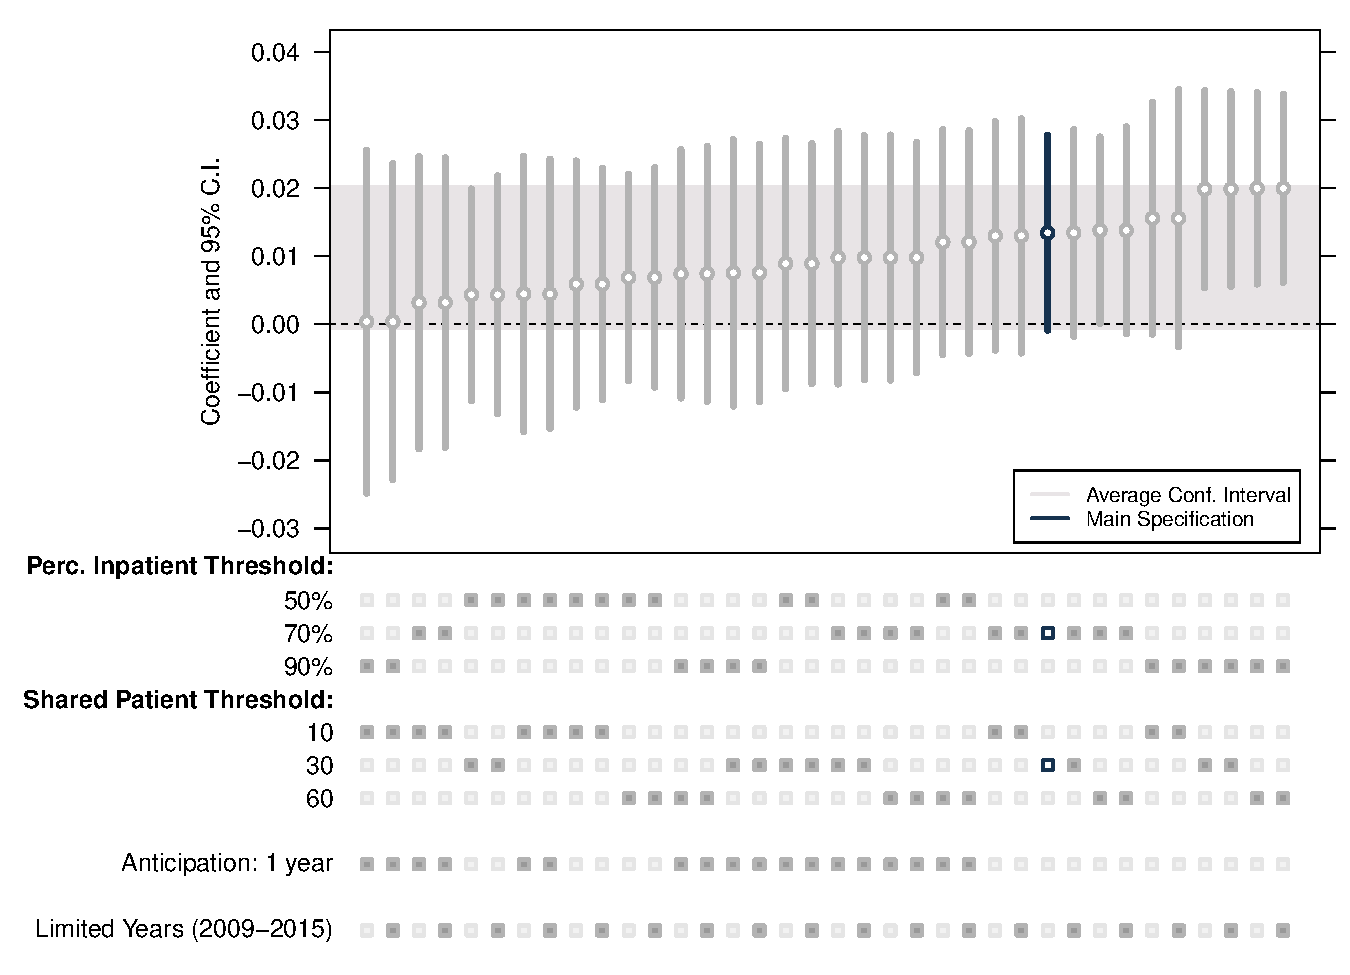
\includegraphics[width=0.9\textwidth]{Objects/spec_chart_retired_ever.pdf}
    \label{fig:retire_chart}
        \caption*{\footnotesize{\textit{Notes:} The figure summarizes estimates across alternative specifications. Points indicate coefficient estimates and bars indicate 95\% confidence intervals.}}
\end{figure}

\subsubsection{Change Work Setting}

Figure \ref{fig:work_chart} presents the effect of EHR exposure on the likelihood of working in an office setting under different combinations of specification choices. The main specification yields an average treatment effect of 0.115, toward the upper end of the range produced by alternative specifications, which cluster between roughly 0.05 and 0.13. Every specification yields a positive and statistically significant effect. Limiting the sample to 2009--2015 and allowing for one year of anticipation both push the estimate toward the lower end of this range, but do not change its sign or significance.

\begin{figure}[ht!]
    \caption{Outcome: Work in Office}
    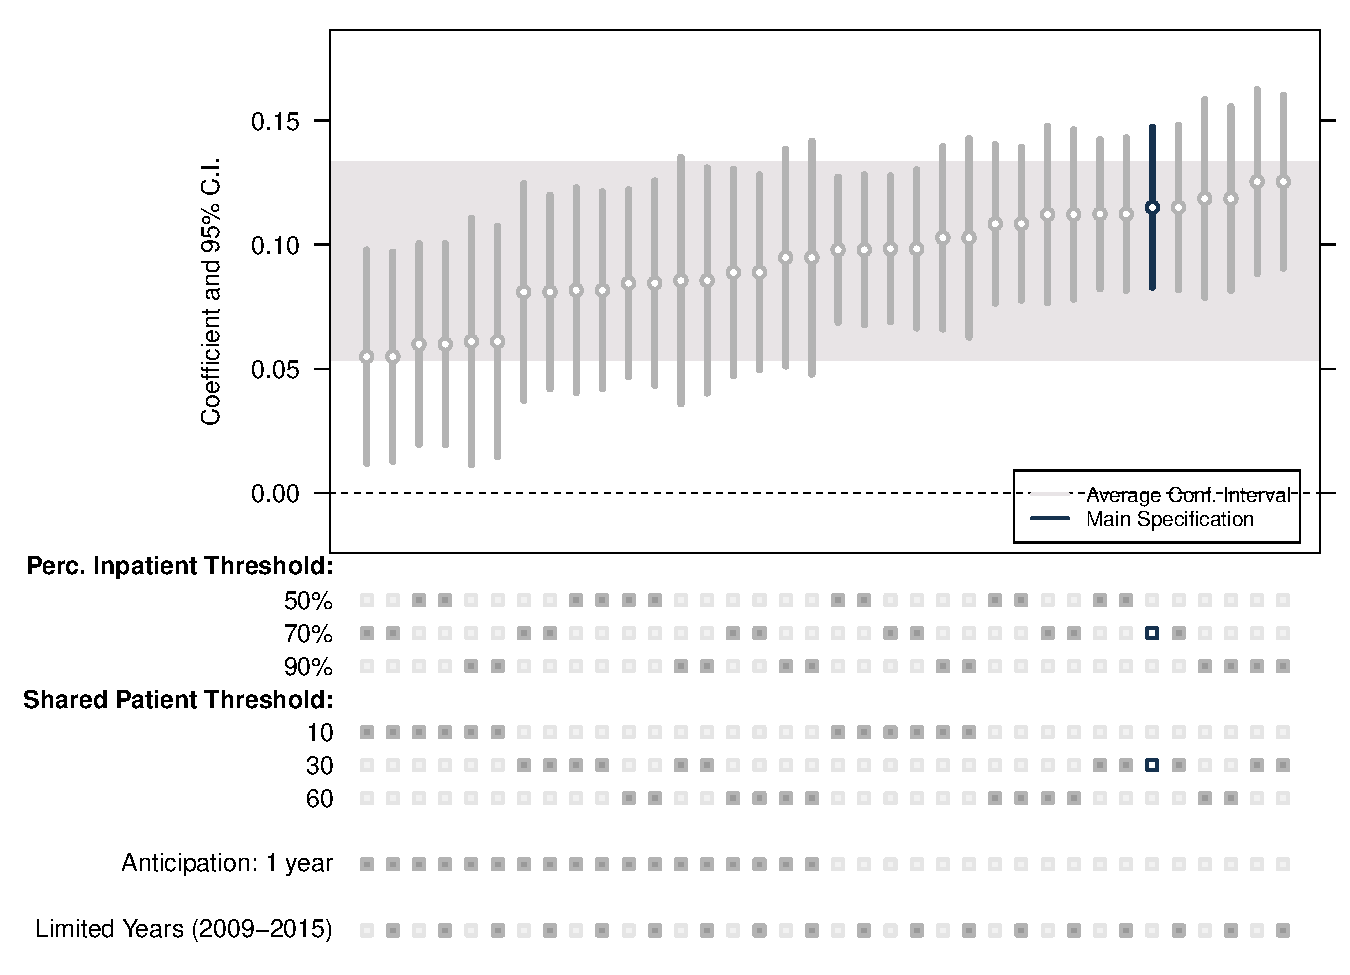
\includegraphics[width=0.9\textwidth]{Objects/spec_chart_work_in_office.pdf}
    \label{fig:work_chart}
            \caption*{\footnotesize{\textit{Notes:} The figure summarizes estimates across alternative specifications. Points indicate coefficient estimates and bars indicate 95\% confidence intervals.}}
\end{figure}

Now I turn to whether hospitalists change the fraction of patients seen in an office setting following EHR exposure. Figure \ref{fig:fracoffice_chart} presents these results under the same set of specification changes. The main specification yields an average treatment effect of 0.111, again toward the upper end of the range produced by alternative specifications, which cluster between roughly 0.04 and 0.13. As with the indicator for working in an office, every specification yields a positive and statistically significant effect, and limiting the sample years or allowing for anticipation both push the magnitude of the estimate down without changing its sign or significance.

\begin{figure}[ht!]
\centering
    \caption{Outcome: Fraction of Claims in Office}
    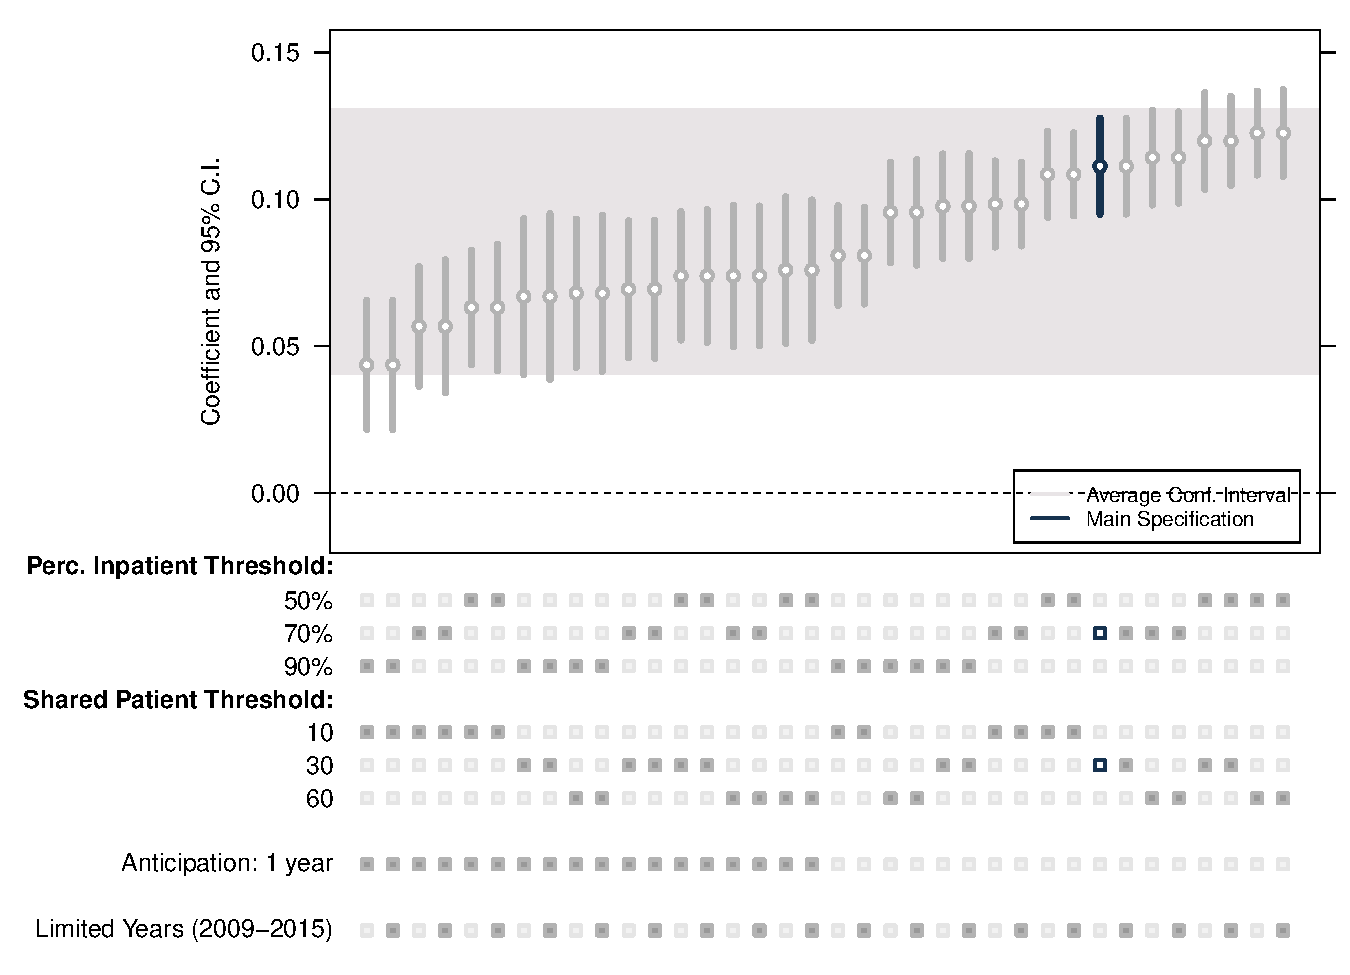
\includegraphics[width=0.9\textwidth]{Objects/spec_chart_pos_office.pdf}
    \label{fig:fracoffice_chart}
            \caption*{\footnotesize{\textit{Notes:} The figure summarizes estimates across alternative specifications. Points indicate coefficient estimates and bars indicate 95\% confidence intervals.}}
\end{figure}



\subsubsection{Patient Count and Claims per Patient}

Figure \ref{fig:pat_chart} presents estimates of the effect of EHR exposure on patient count under different combinations of specification changes. The main specification yields an average treatment effect of 18.5 additional patients, falling within the middle-to-upper range of estimates produced by alternative specifications, which range from roughly $-5$ to $25$. Unlike the exit and office-setting outcomes, a subset of the more restrictive specifications, particularly those combining a higher shared-patient threshold with a higher inpatient-share threshold, produce point estimates that are not statistically distinguishable from zero, though none is meaningfully negative. The main specification's estimate is broadly consistent with the majority of alternative specifications, which support a positive effect of EHR exposure on patient count.

\begin{figure}[ht!]
\centering
    \caption{Outcome: Patient Count}
    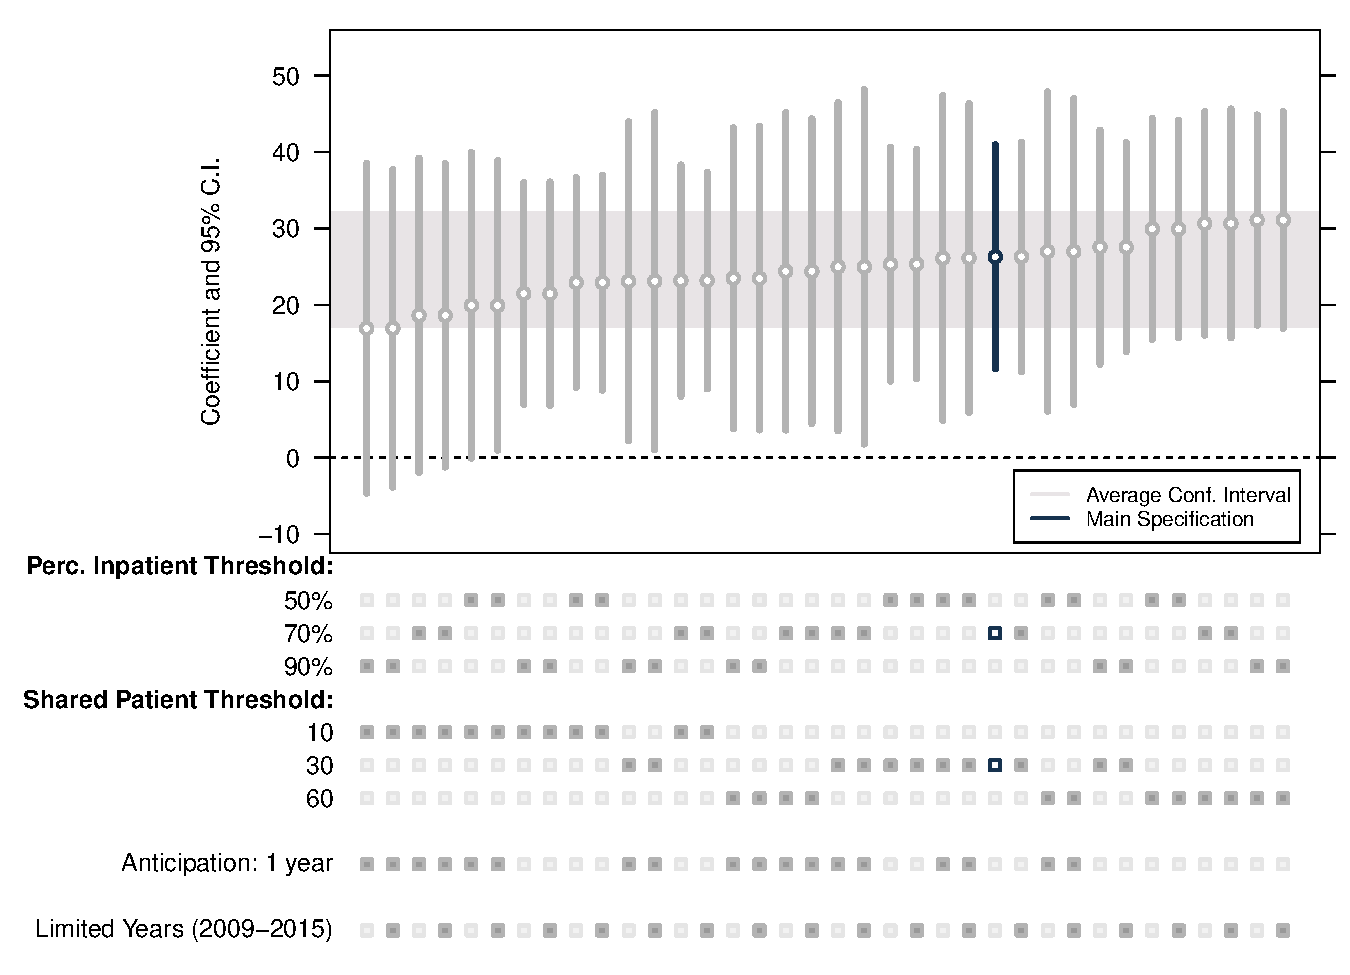
\includegraphics[width=0.9\textwidth]{Objects/spec_chart_npi_unq_benes.pdf}
    \label{fig:pat_chart}
            \caption*{\footnotesize{\textit{Notes:} The figure summarizes estimates across alternative specifications. Points indicate coefficient estimates and bars indicate 95\% confidence intervals.}}
\end{figure}


\begin{figure}[ht!]
\centering
    \captionsetup{width=.9\linewidth}
    \caption{Effect of EHR Exposure on Claims per Patient}
   \begin{subfigure}[]{.9\textwidth}
   \centering
   \caption{Full Sample}
   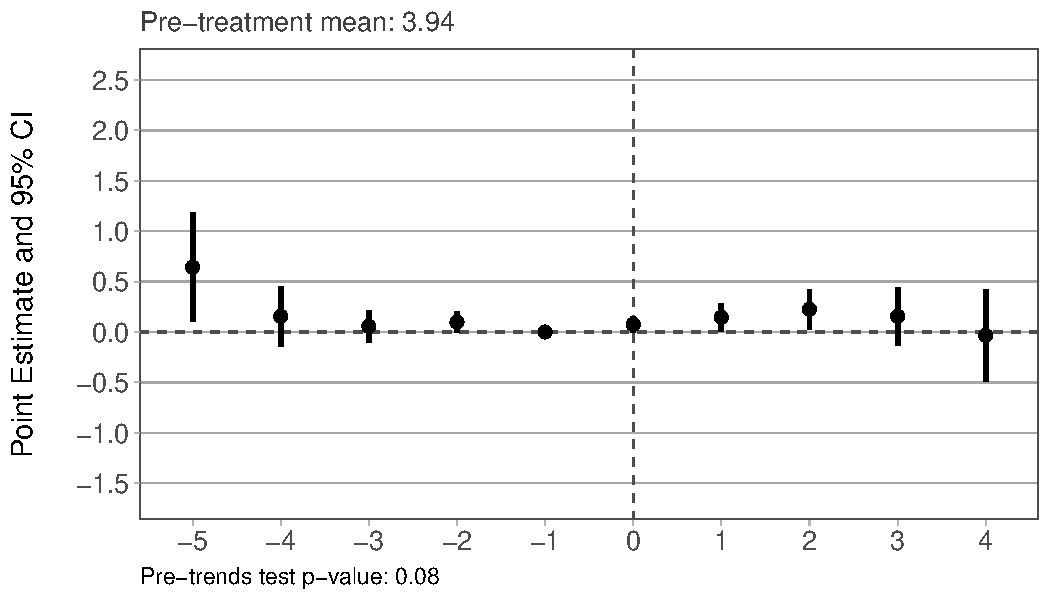
\includegraphics[width=0.9\textwidth]{Objects/claim_per_patient_plot_all_new.pdf}
   \label{fig:claima} 
\end{subfigure}

\vspace{3mm}

\begin{subfigure}[]{.9\textwidth}
\centering
\caption{Heterogeneity by Age}
   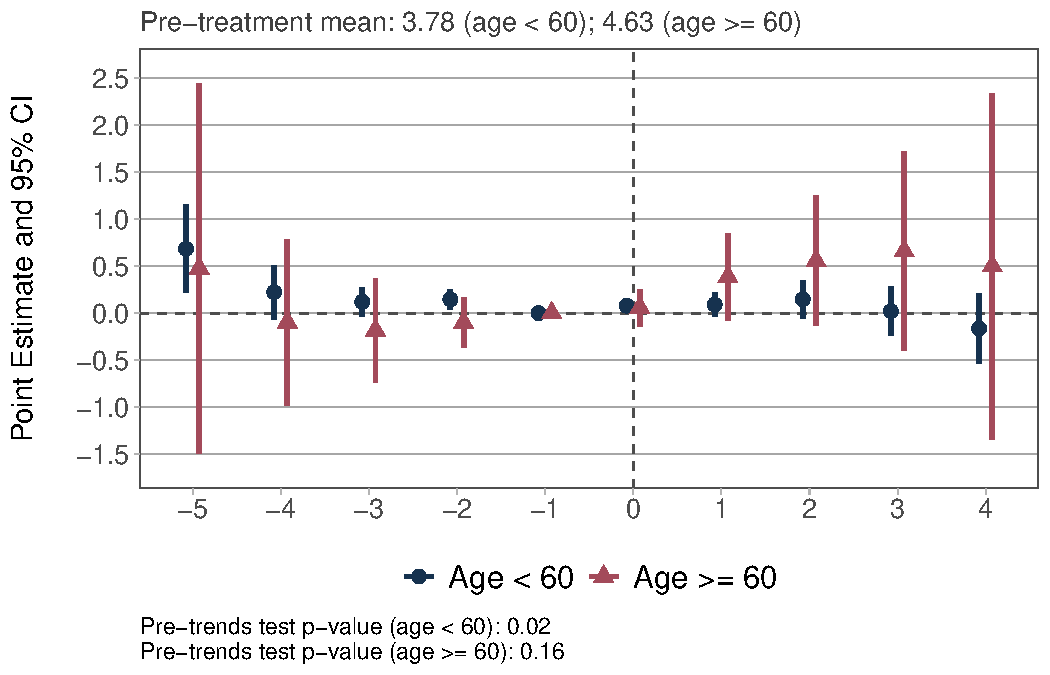
\includegraphics[width=0.9\textwidth]{Objects/claim_per_patient_plot_ages_new.pdf}
   \label{fig:claimb}
\end{subfigure}
\label{fig:claim}
\vspace{2mm}
    \caption*{\footnotesize{\textit{Notes:} The top panel shows average group time treatment effects aggregated over groups to an event study plot. The bottom show these results for different subgroups of physicians by age. The p-value listed for each graph corresponds to a Wald test for pre-trends. Confidence intervals shown are pointwise 95\% intervals. Overall ATT for all, $<$ 60, $>=$ 60 with SE in parentheses: -0.246 (0.096), -0.232 (0.084), -0.372 (0.523), respectively.}}
\end{figure}

I examine estimates of the effect of EHR exposure on claims per patient under the same set of specification changes, shown in Figure \ref{fig:cpp_chart}. The main specification yields an average treatment effect of $-0.246$, indicating a decrease in claims filed per patient following EHR exposure. Most alternative specifications are also negative and of similar magnitude, clustering between roughly $-0.4$ and $-0.1$; a smaller subset of specifications, generally those combining a higher shared-patient threshold with a higher inpatient-share threshold, produce estimates closer to zero or, in a few cases, marginally positive, though these confidence intervals are wide and consistent with either a null or negative effect. Given that this pattern is broadly consistent across most specifications, I interpret this as suggestive evidence that EHR exposure is associated with a decrease in claims per patient, though the magnitude is sensitive to sample restrictions.

\begin{figure}[ht!]
    \caption{Outcome: Claims per Patient}
    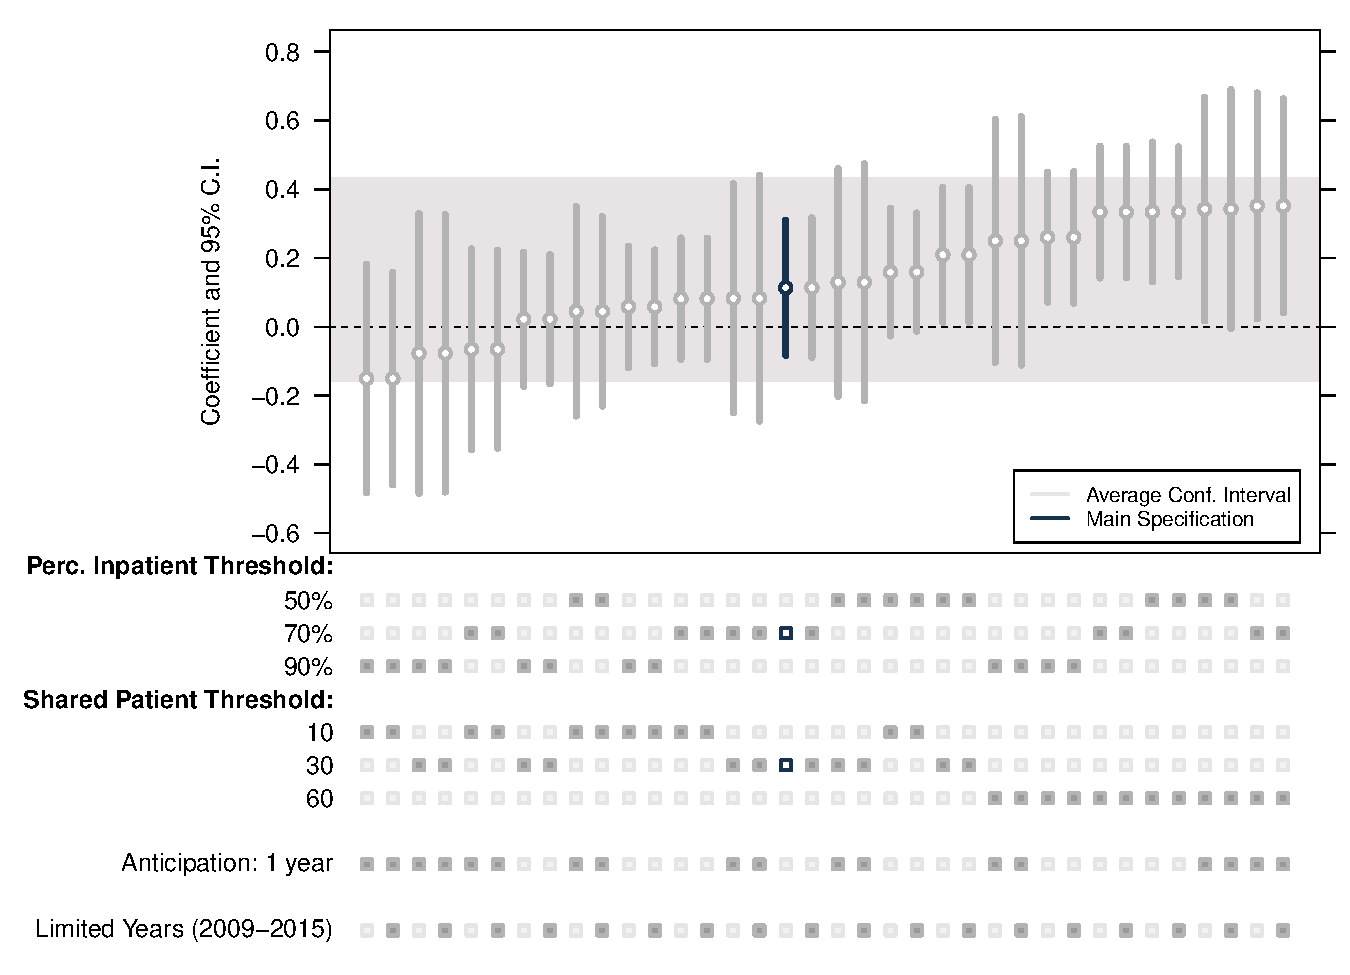
\includegraphics[width=0.9\textwidth]{Objects/spec_chart_claim_per_patient.pdf}
    \label{fig:cpp_chart}
            \caption*{\footnotesize{\textit{Notes:} The figure summarizes estimates across alternative specifications. Points indicate coefficient estimates and bars indicate 95\% confidence intervals.}}
\end{figure}

\clearpage

\section{Event Study Estimates}\label{sec:eventstudyestimates}


\begin{landscape}\begin{table}[!h]
\centering
\caption{\label{tab:ci_retired_ever}Event-time estimates and confidence intervals: Exit from Clinical Practice}
\centering
\fontsize{9}{11}\selectfont
\begin{tabular}[t]{lccccccccc}
\toprule
\multicolumn{1}{c}{ } & \multicolumn{9}{c}{Event time relative to first EHR exposure} \\
\cmidrule(l{3pt}r{3pt}){2-10}
 & -5 & -4 & -3 & -2 & 0 & 1 & 2 & 3 & 4\\
\midrule
\addlinespace[0.3em]
\multicolumn{10}{l}{\textbf{Age $<$ 60}}\\
\hspace{1em}Estimate & 0.021 & 0.005 & 0.005 & 0.000 & 0.001 & 0.006 & 0.011 & 0.017 & 0.003\\
\hspace{1em}95\% CI & {}[-0.012, 0.054] & {}[-0.012, 0.022] & {}[-0.004, 0.013] & {}[-0.004, 0.005] & {}[-0.003, 0.004] & {}[-0.001, 0.013] & {}[-0.003, 0.025] & {}[-0.004, 0.038] & {}[-0.033, 0.038]\\
\hspace{1em}CI width & 0.066 & 0.034 & 0.017 & 0.009 & 0.007 & 0.014 & 0.029 & 0.041 & 0.071\\
\hspace{1em}Physicians & 491 & 989 & 1,841 & 2,995 & 4,419 & 4,419 & 4,419 & 4,277 & 3,928\\
\hspace{1em}Events & 0 & 2 & 7 & 14 & 61 & 122 & 203 & 271 & 300\\
\addlinespace[0.3em]
\multicolumn{10}{l}{\textbf{Age $\geq$ 60}}\\
\hspace{1em}Estimate & 0.015 & 0.007 & -0.001 & -0.002 & 0.003 & 0.031 & 0.044 & 0.060 & 0.075\\
\hspace{1em}95\% CI & {}[-0.075, 0.105] & {}[-0.038, 0.051] & {}[-0.031, 0.030] & {}[-0.015, 0.012] & {}[-0.006, 0.012] & {}[0.009, 0.052] & {}[0.004, 0.084] & {}[0.001, 0.118] & {}[-0.013, 0.162]\\
\hspace{1em}CI width & 0.180 & 0.089 & 0.061 & 0.027 & 0.018 & 0.044 & 0.080 & 0.117 & 0.175\\
\hspace{1em}Physicians & 134 & 273 & 470 & 760 & 1,052 & 1,052 & 1,052 & 1,016 & 918\\
\hspace{1em}Events & 0 & 0 & 3 & 9 & 34 & 79 & 120 & 158 & 176\\
\addlinespace[0.3em]
\multicolumn{10}{l}{\textbf{All}}\\
\hspace{1em}Estimate & 0.019 & 0.005 & 0.004 & 0.000 & 0.001 & 0.010 & 0.017 & 0.024 & 0.015\\
\hspace{1em}95\% CI & {}[-0.014, 0.053] & {}[-0.011, 0.022] & {}[-0.005, 0.013] & {}[-0.004, 0.004] & {}[-0.002, 0.004] & {}[0.003, 0.017] & {}[0.003, 0.030] & {}[0.004, 0.045] & {}[-0.021, 0.051]\\
\hspace{1em}CI width & 0.067 & 0.033 & 0.018 & 0.009 & 0.007 & 0.015 & 0.027 & 0.041 & 0.072\\
\hspace{1em}Physicians & 625 & 1,262 & 2,311 & 3,755 & 5,471 & 5,471 & 5,471 & 5,293 & 4,846\\
\hspace{1em}Events & 0 & 2 & 10 & 23 & 95 & 201 & 323 & 429 & 476\\
\bottomrule
\end{tabular}
\begin{tablenotes}
\item \textit{Note: } This table provides the exact numerical estimates underlying the corresponding event-study figure from the main specification. Coefficients are measured relative to the year before first EHR exposure (event time -1). Brackets report 95\% confidence intervals. 
\end{tablenotes}
\end{table}
\end{landscape}



\begin{landscape}\begin{table}[!h]
\centering
\caption{\label{tab:ci_work_in_office}Event-time estimates and confidence intervals: Works in an Office}
\centering
\fontsize{9}{11}\selectfont
\begin{tabular}[t]{lccccccccc}
\toprule
\multicolumn{1}{c}{ } & \multicolumn{9}{c}{Event time relative to first EHR exposure} \\
\cmidrule(l{3pt}r{3pt}){2-10}
 & -5 & -4 & -3 & -2 & 0 & 1 & 2 & 3 & 4\\
\midrule
\addlinespace[0.3em]
\multicolumn{10}{l}{\textbf{All}}\\
\hspace{1em}Estimate & 0.065 & -0.005 & -0.005 & -0.004 & 0.053 & 0.083 & 0.123 & 0.164 & 0.152\\
\hspace{1em}95\% CI & {}[-0.020, 0.149] & {}[-0.050, 0.040] & {}[-0.031, 0.021] & {}[-0.022, 0.013] & {}[0.039, 0.066] & {}[0.063, 0.104] & {}[0.093, 0.154] & {}[0.117, 0.211] & {}[0.078, 0.226]\\
\hspace{1em}CI width & 0.169 & 0.089 & 0.052 & 0.035 & 0.028 & 0.042 & 0.060 & 0.094 & 0.147\\
\addlinespace[0.3em]
\multicolumn{10}{l}{\textbf{Age $<$ 60}}\\
\hspace{1em}Estimate & 0.079 & 0.017 & -0.003 & -0.003 & 0.046 & 0.071 & 0.108 & 0.146 & 0.125\\
\hspace{1em}95\% CI & {}[-0.014, 0.171] & {}[-0.029, 0.064] & {}[-0.032, 0.026] & {}[-0.021, 0.014] & {}[0.030, 0.062] & {}[0.049, 0.094] & {}[0.077, 0.139] & {}[0.099, 0.193] & {}[0.042, 0.207]\\
\hspace{1em}CI width & 0.185 & 0.093 & 0.057 & 0.035 & 0.032 & 0.045 & 0.062 & 0.094 & 0.165\\
\addlinespace[0.3em]
\multicolumn{10}{l}{\textbf{Age $\geq$ 60}}\\
\hspace{1em}Estimate & 0.010 & -0.093 & -0.012 & -0.008 & 0.080 & 0.135 & 0.188 & 0.233 & 0.250\\
\hspace{1em}95\% CI & {}[-0.189, 0.210] & {}[-0.209, 0.023] & {}[-0.078, 0.055] & {}[-0.053, 0.037] & {}[0.047, 0.114] & {}[0.087, 0.184] & {}[0.116, 0.260] & {}[0.117, 0.349] & {}[0.068, 0.433]\\
\hspace{1em}CI width & 0.399 & 0.232 & 0.133 & 0.090 & 0.067 & 0.098 & 0.145 & 0.232 & 0.365\\
\bottomrule
\end{tabular}
\begin{tablenotes}
\item \textit{Note: } This table provides the exact numerical estimates underlying the corresponding event-study figure from the main specification. Coefficients are measured relative to the year before first EHR exposure (event time -1). Brackets report 95\% confidence intervals. 
\end{tablenotes}
\end{table}
\end{landscape}



\begin{landscape}\begin{table}[!h]
\centering
\caption{\label{tab:ci_pos_office}Event-time estimates and confidence intervals: Fraction of Claims in Office}
\centering
\fontsize{9}{11}\selectfont
\begin{tabular}[t]{lccccccccc}
\toprule
\multicolumn{1}{c}{ } & \multicolumn{9}{c}{Event time relative to first EHR exposure} \\
\cmidrule(l{3pt}r{3pt}){2-10}
 & -5 & -4 & -3 & -2 & 0 & 1 & 2 & 3 & 4\\
\midrule
\addlinespace[0.3em]
\multicolumn{10}{l}{\textbf{All}}\\
\hspace{1em}Estimate & 0.031 & 0.001 & -0.000 & 0.004 & 0.046 & 0.081 & 0.113 & 0.148 & 0.167\\
\hspace{1em}95\% CI & {}[-0.015, 0.078] & {}[-0.024, 0.027] & {}[-0.014, 0.013] & {}[-0.003, 0.011] & {}[0.041, 0.051] & {}[0.072, 0.091] & {}[0.097, 0.128] & {}[0.124, 0.173] & {}[0.129, 0.205]\\
\hspace{1em}CI width & 0.093 & 0.050 & 0.026 & 0.014 & 0.010 & 0.018 & 0.031 & 0.048 & 0.076\\
\addlinespace[0.3em]
\multicolumn{10}{l}{\textbf{Age $<$ 60}}\\
\hspace{1em}Estimate & 0.038 & 0.016 & 0.005 & 0.006 & 0.043 & 0.076 & 0.103 & 0.131 & 0.145\\
\hspace{1em}95\% CI & {}[-0.007, 0.084] & {}[-0.008, 0.040] & {}[-0.009, 0.019] & {}[-0.001, 0.013] & {}[0.038, 0.049] & {}[0.067, 0.086] & {}[0.088, 0.118] & {}[0.107, 0.155] & {}[0.109, 0.180]\\
\hspace{1em}CI width & 0.090 & 0.048 & 0.028 & 0.014 & 0.011 & 0.019 & 0.031 & 0.048 & 0.071\\
\addlinespace[0.3em]
\multicolumn{10}{l}{\textbf{Age $\geq$ 60}}\\
\hspace{1em}Estimate & 0.003 & -0.055 & -0.023 & -0.003 & 0.060 & 0.103 & 0.151 & 0.220 & 0.259\\
\hspace{1em}95\% CI & {}[-0.130, 0.137] & {}[-0.131, 0.021] & {}[-0.058, 0.012] & {}[-0.022, 0.016] & {}[0.045, 0.075] & {}[0.077, 0.129] & {}[0.108, 0.193] & {}[0.143, 0.297] & {}[0.138, 0.379]\\
\hspace{1em}CI width & 0.267 & 0.153 & 0.070 & 0.037 & 0.030 & 0.052 & 0.085 & 0.153 & 0.241\\
\bottomrule
\end{tabular}
\begin{tablenotes}
\item \textit{Note: } This table provides the exact numerical estimates underlying the corresponding event-study figure from the main specification. Coefficients are measured relative to the year before first EHR exposure (event time -1). Brackets report 95\% confidence intervals. 
\end{tablenotes}
\end{table}
\end{landscape}



\begin{landscape}\begin{table}[!h]
\centering
\caption{\label{tab:ci_npi_unq_benes}Event-time estimates and confidence intervals: Number of Patients}
\centering
\fontsize{9}{11}\selectfont
\begin{tabular}[t]{lccccccccc}
\toprule
\multicolumn{1}{c}{ } & \multicolumn{9}{c}{Event time relative to first EHR exposure} \\
\cmidrule(l{3pt}r{3pt}){2-10}
 & -5 & -4 & -3 & -2 & 0 & 1 & 2 & 3 & 4\\
\midrule
\addlinespace[0.3em]
\multicolumn{10}{l}{\textbf{All}}\\
\hspace{1em}Estimate & 19.262 & -3.032 & -0.034 & 5.760 & 3.844 & 14.671 & 19.750 & 24.898 & 29.443\\
\hspace{1em}95\% CI & {}[-27.45, 65.97] & {}[-25.85, 19.79] & {}[-13.34, 13.27] & {}[-1.89, 13.41] & {}[-3.02, 10.71] & {}[3.88, 25.46] & {}[4.59, 34.91] & {}[3.05, 46.74] & {}[-5.13, 64.01]\\
\hspace{1em}CI width & 93.416 & 45.644 & 26.605 & 15.304 & 13.730 & 21.576 & 30.314 & 43.687 & 69.149\\
\addlinespace[0.3em]
\multicolumn{10}{l}{\textbf{Age $<$ 60}}\\
\hspace{1em}Estimate & 2.393 & 2.004 & 2.577 & 5.491 & 3.731 & 15.261 & 19.872 & 23.862 & 39.613\\
\hspace{1em}95\% CI & {}[-41.18, 45.96] & {}[-22.83, 26.84] & {}[-11.06, 16.21] & {}[-2.75, 13.74] & {}[-3.86, 11.32] & {}[3.65, 26.86] & {}[3.29, 36.44] & {}[1.44, 46.27] & {}[1.45, 77.77]\\
\hspace{1em}CI width & 87.151 & 49.674 & 27.282 & 16.496 & 15.185 & 23.208 & 33.147 & 44.827 & 76.321\\
\addlinespace[0.3em]
\multicolumn{10}{l}{\textbf{Age $\geq$ 60}}\\
\hspace{1em}Estimate & 112.738 & -26.037 & -12.202 & 8.980 & 5.695 & 8.293 & 11.193 & 22.107 & -47.440\\
\hspace{1em}95\% CI & {}[-47.55, 273.02] & {}[-95.08, 43.01] & {}[-57.20, 32.80] & {}[-15.05, 33.01] & {}[-12.33, 23.73] & {}[-21.61, 38.19] & {}[-27.73, 50.11] & {}[-35.91, 80.13] & {}[-158.24, 63.36]\\
\hspace{1em}CI width & 320.579 & 138.097 & 90.012 & 48.073 & 36.070 & 59.808 & 77.851 & 116.045 & 221.600\\
\bottomrule
\end{tabular}
\begin{tablenotes}
\item \textit{Note: } This table provides the exact numerical estimates underlying the corresponding event-study figure from the main specification. Coefficients are measured relative to the year before first EHR exposure (event time -1). Brackets report 95\% confidence intervals. 
\end{tablenotes}
\end{table}
\end{landscape}



\begin{landscape}\begin{table}[!h]
\centering
\caption{\label{tab:ci_claim_per_patient}Event-time estimates and confidence intervals: Claims per Patient}
\centering
\fontsize{9}{11}\selectfont
\begin{tabular}[t]{lccccccccc}
\toprule
\multicolumn{1}{c}{ } & \multicolumn{9}{c}{Event time relative to first EHR exposure} \\
\cmidrule(l{3pt}r{3pt}){2-10}
 & -5 & -4 & -3 & -2 & 0 & 1 & 2 & 3 & 4\\
\midrule
\addlinespace[0.3em]
\multicolumn{10}{l}{\textbf{All}}\\
\hspace{1em}Estimate & 0.795 & 0.377 & 0.194 & 0.115 & 0.039 & -0.105 & -0.237 & -0.381 & -0.547\\
\hspace{1em}95\% CI & {}[0.245, 1.345] & {}[0.078, 0.676] & {}[0.056, 0.331] & {}[0.032, 0.197] & {}[-0.037, 0.115] & {}[-0.223, 0.013] & {}[-0.405, -0.069] & {}[-0.647, -0.115] & {}[-1.055, -0.039]\\
\hspace{1em}CI width & 1.100 & 0.598 & 0.275 & 0.165 & 0.152 & 0.235 & 0.335 & 0.533 & 1.016\\
\addlinespace[0.3em]
\multicolumn{10}{l}{\textbf{Age $<$ 60}}\\
\hspace{1em}Estimate & 0.980 & 0.381 & 0.190 & 0.116 & 0.053 & -0.099 & -0.198 & -0.346 & -0.570\\
\hspace{1em}95\% CI & {}[0.592, 1.368] & {}[0.166, 0.597] & {}[0.065, 0.315] & {}[0.042, 0.191] & {}[-0.028, 0.134] & {}[-0.206, 0.008] & {}[-0.354, -0.043] & {}[-0.574, -0.118] & {}[-0.951, -0.189]\\
\hspace{1em}CI width & 0.777 & 0.432 & 0.250 & 0.150 & 0.162 & 0.214 & 0.310 & 0.456 & 0.762\\
\addlinespace[0.3em]
\multicolumn{10}{l}{\textbf{Age $\geq$ 60}}\\
\hspace{1em}Estimate & -0.186 & 0.278 & 0.125 & 0.036 & -0.074 & -0.147 & -0.468 & -0.618 & -0.553\\
\hspace{1em}95\% CI & {}[-3.284, 2.912] & {}[-1.529, 2.084] & {}[-0.706, 0.956] & {}[-0.316, 0.388] & {}[-0.305, 0.157] & {}[-0.765, 0.470] & {}[-1.322, 0.385] & {}[-2.205, 0.969] & {}[-2.930, 1.825]\\
\hspace{1em}CI width & 6.196 & 3.613 & 1.662 & 0.705 & 0.463 & 1.234 & 1.707 & 3.174 & 4.755\\
\bottomrule
\end{tabular}
\begin{tablenotes}
\item \textit{Note: } This table provides the exact numerical estimates underlying the corresponding event-study figure from the main specification. Coefficients are measured relative to the year before first EHR exposure (event time -1). Brackets report 95\% confidence intervals. 
\end{tablenotes}
\end{table}
\end{landscape}


\section{De-Aggregated Event Study Plots}

\begin{figure}[ht!]
    \centering
    \caption{Effect of EHR Exposure on Exiting Clinical Setting by Group}
    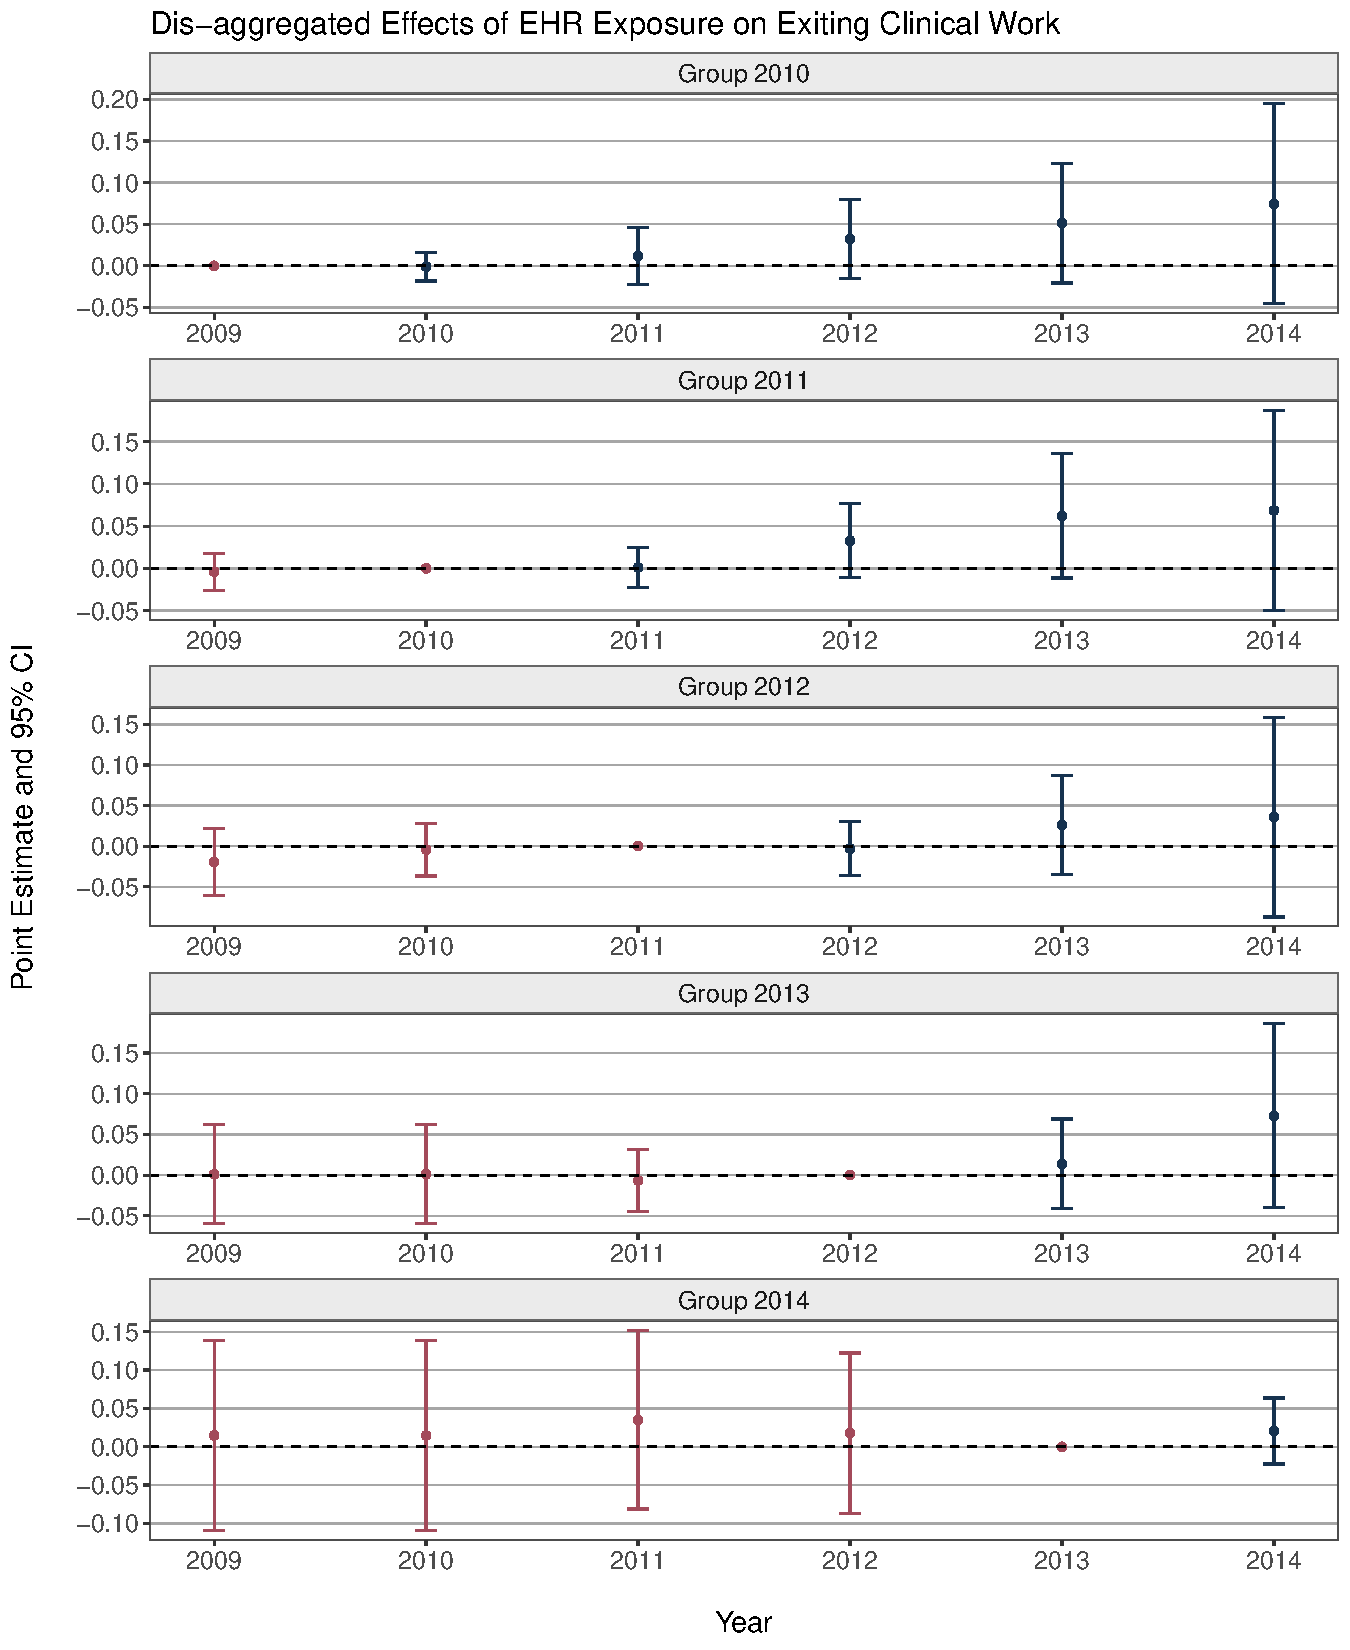
\includegraphics[width=0.65\linewidth]{Objects/retire_group.pdf}
    \label{fig:retire_group}
    \caption*{\footnotesize{\textit{Notes:} Plot shows average group time treatment effects for each treatment group.}}
\end{figure}

\begin{figure}[ht!]
    \centering
    \caption{Effect of EHR Exposure on Working in Office by Group}
    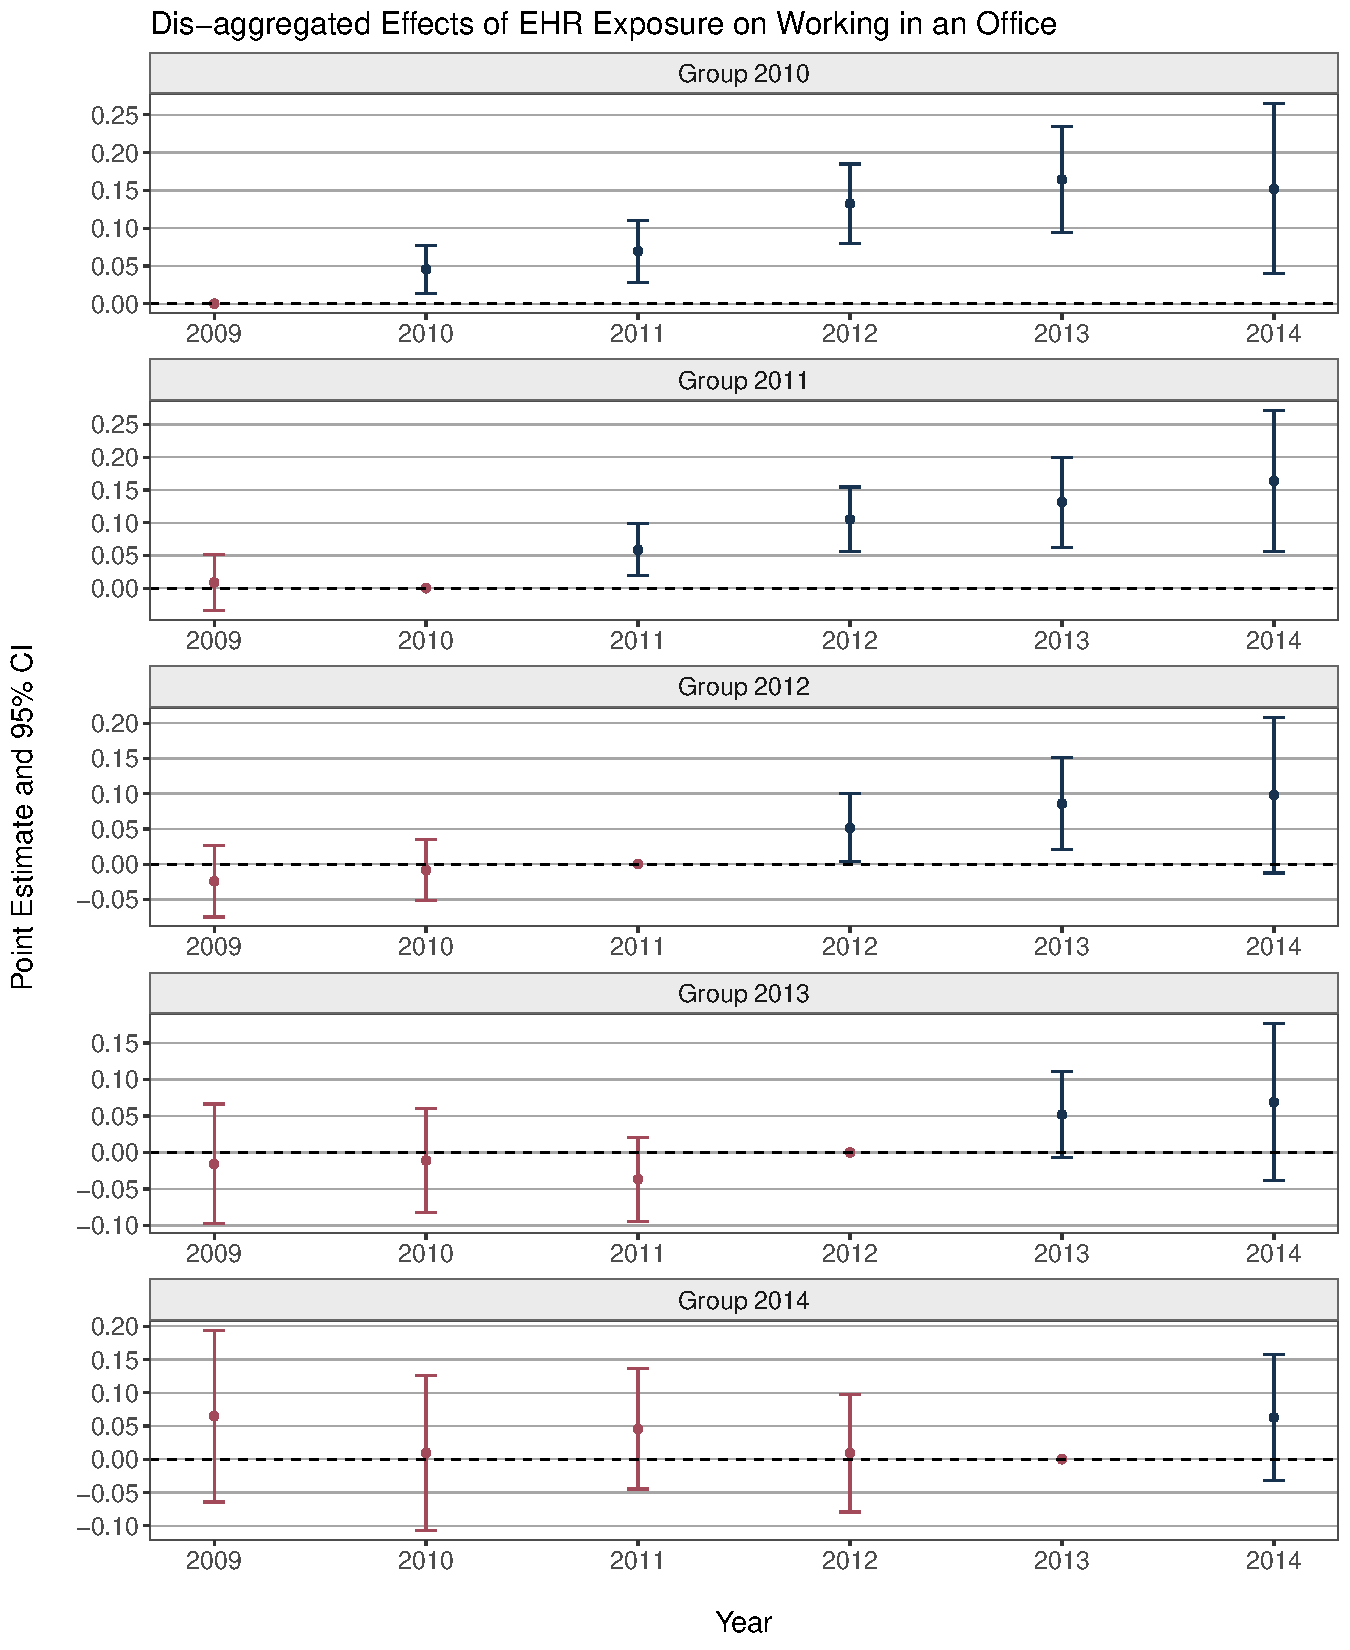
\includegraphics[width=0.65\linewidth]{Objects/officeind_group.pdf}
    \label{fig:officeind_group}
    \caption*{\footnotesize{\textit{Notes:} Plot shows average group time treatment effects for each treatment group.}}
\end{figure}

\begin{figure}[ht!]
    \centering
    \caption{Effect of EHR Exposure on Frac Claims in Office by Group}
    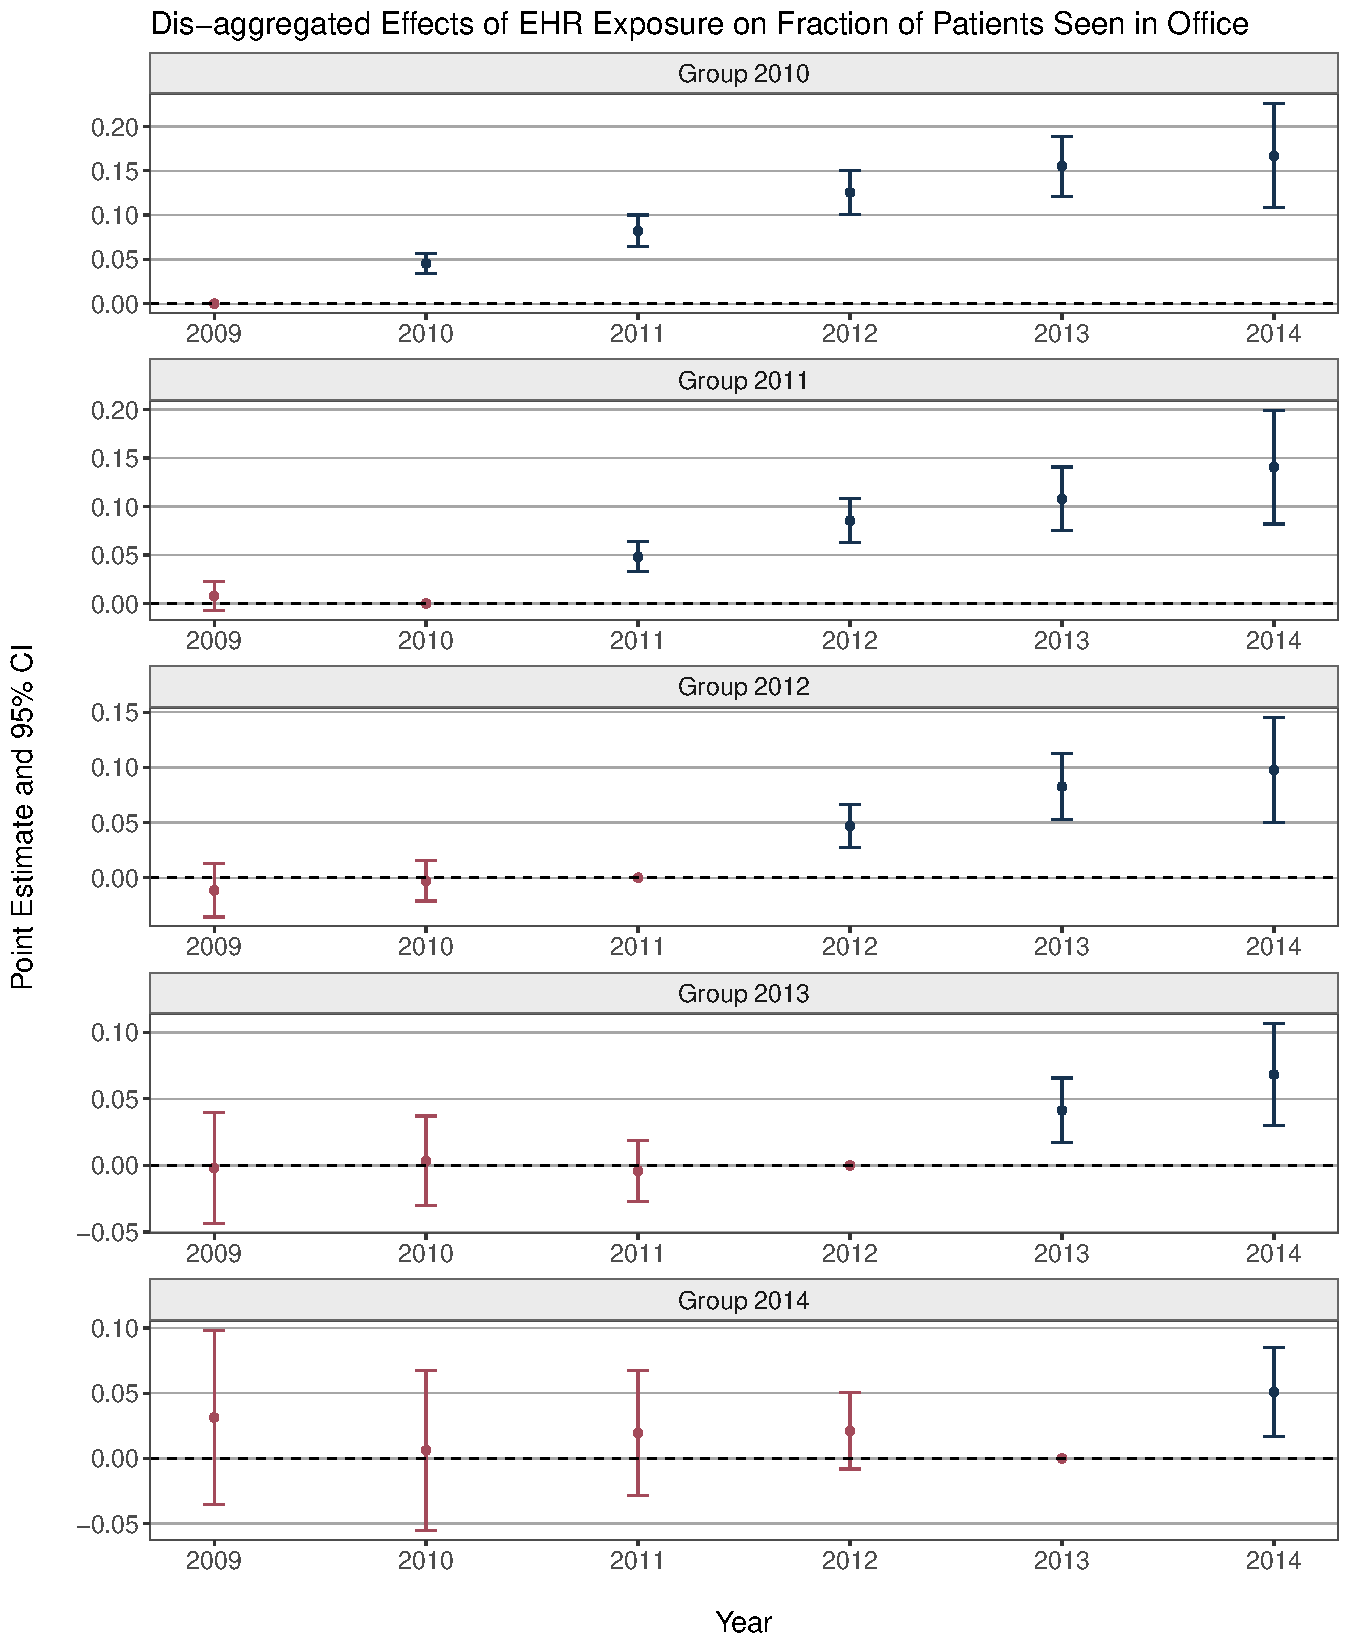
\includegraphics[width=0.65\linewidth]{Objects/officefrac_group.pdf}
    \label{fig:officefrac_group}
    \caption*{\footnotesize{\textit{Notes:} Plot shows average group time treatment effects for each treatment group.}}
\end{figure}

\begin{figure}[ht!]
    \centering
    \captionsetup{width=.6\linewidth}
    \caption{Effect of EHR Exposure on Patient Count by Group}
    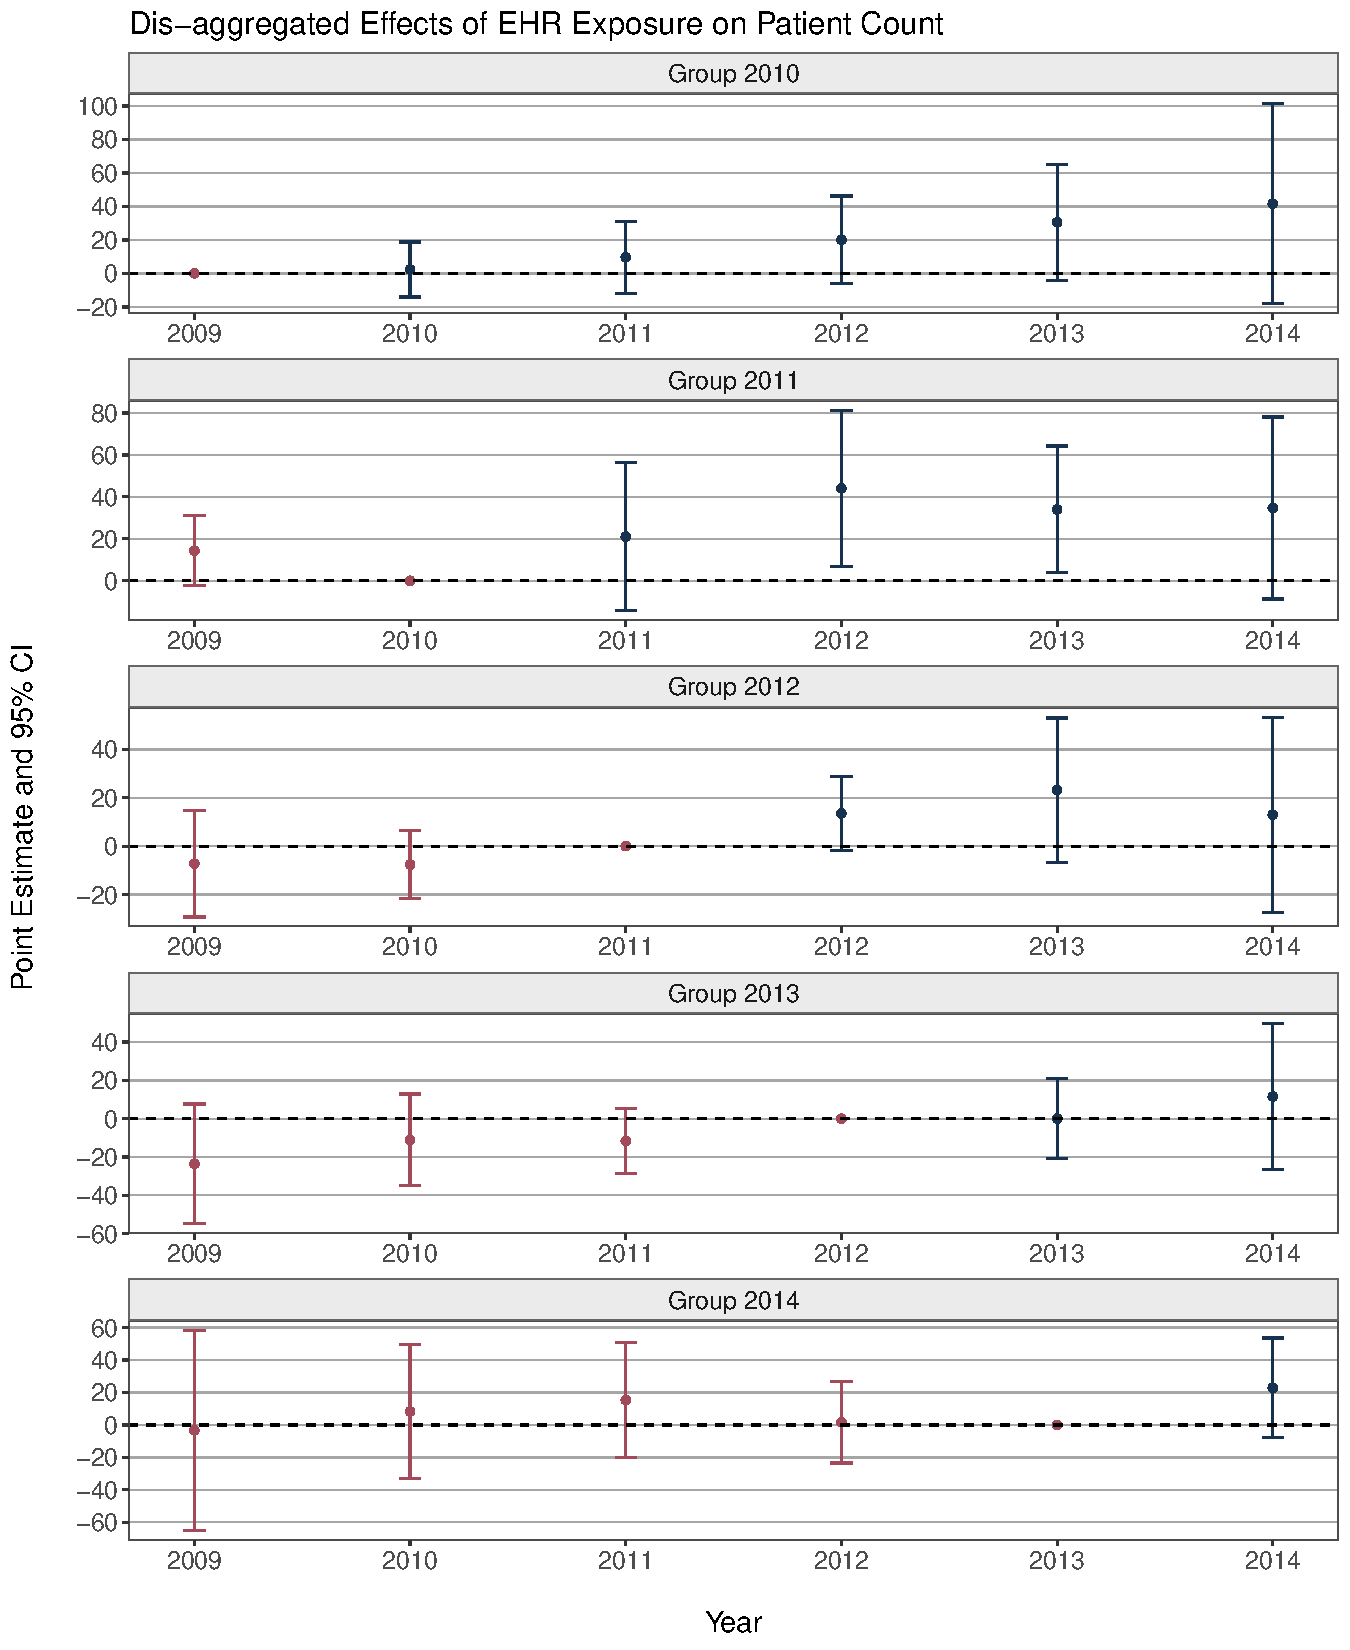
\includegraphics[width=.65\textwidth]{Objects/patient_group.pdf}
    \label{fig:patientgroup}
    \vspace{2mm}
    \caption*{\footnotesize{\textit{Notes:} Plot shows average group time treatment effects for each treatment group.}}
\end{figure}

















\end{document}